\documentclass[11pt]{article}
\usepackage{epsfig}
\usepackage{graphicx}
\usepackage{rotating}
\usepackage{amsmath,amsthm}
\usepackage{array}
\usepackage{multirow}
\usepackage{url}
\usepackage{appendix}
\usepackage{algorithm}
\usepackage{algorithmic}
\usepackage{placeins}  % FloatBarrier
\usepackage{comment}
\usepackage{enumerate} % Fancy enumeration
\usepackage{appendix}
\usepackage{listings}

\setcounter{secnumdepth}{5}
\setcounter{tocdepth}{5}


\usepackage{float}
\floatstyle{boxed}
\restylefloat{figure}
\usepackage{morefloats}

\usepackage{caption}


\lstset{breaklines=true}


\oddsidemargin=0in
\evensidemargin=0in
\textwidth=6.5in
%\textwidth=6.42in (if no footnote)
\textheight=8.75in
%\textheight=9.1in (if no footnote)
%\topmargin=-0.5cm
%\topmargin=0.5in
\footskip=1.0cm
\headheight=0pt
%\newcommand{\comment}[1]{}

\setlength{\extrarowheight}{5pt}

\theoremstyle{definition}
\newtheorem{definition}{Definition}
\newtheorem*{examples}{Examples}
\newtheorem{example}{}

\begin{document}

\title{Incremental Time Series Denoising}

\date{\today}

%

\author{Jeremy Luke Thompson \\
United States Air Force Academy \\
Lawrence Livermore National Laboratory
}

%\vfill
%\vspace{2.0in}
\begin{titlepage}
\maketitle
\end{titlepage}

\tableofcontents

\newpage

\listoffigures

\newpage

\lstlistoflistings

\newpage


\begin{abstract}
In this paper, we focus on denoising techniques for streaming data that are analyzed while being collected. We investigate spatial filters, such as the Box filter, Gaussian smoothing, and the Bilateral filter, frequency techniques, such as Fast Fourier Transform coefficient thresholding and Wavelet Transform coefficient thresholding, and a statistical neighborhood filter, Non-Local Means. These methods are applied to both synthetic data and real world data. We discuss practical concerns for incremental implementation, such as edge treatment, incremental updating, and parameter stability. We note situations when these methods fail and make recommendations for use with real world data, specifically for the use of the Bilateral filter or a combination of the Bilateral and Non-Local Means filters.
\end{abstract}

%\thispagestyle{empty} %\vspace{2.0in}

%\vfill \eject


%\thispagestyle{empty}

%\clearpage

\pagestyle{plain}
\pagenumbering{arabic}


%%%%%%%%%%%%%%%%%%%%%%%%%%%%%%%%%%%%%%%%%%%%%%%%%%%%%%%%%%%%%%%%%%%%%%%%%%


 
\section{Time Series Data and Noise}


\subsection{Time Series Data}

A time series is any temporally ordered series of observations. Frequently, as when collecting observations of various real world phenomenon, the observations will be contaminated with errors, or noise. In this paper, we consider various techniques for denoising time series data received incrementally. We will discuss technique selection, parameter selection and optimization, incremental implementation, and quality assessment. Additionally, we will assess the performance of these techniques in the context of both known signals with added noise and real world data. Frequently, this type of analysis is also known as signal analysis.

\subsection{Noise}

The different assumptions about noise in a time series lend themselves to different denoising techniques.  Generally, noise is assumed to be Additive White Gaussian Noise (AWGN). AWGN is comprised of independent identically distributed real values from the Gaussian distribution with an unknown variance, $\sigma ^2_n$. Many deniosing techniques rely upon an estimate of this unknown noise variance. Gasser, et al.~\cite{Gasser86} describes a method for estimating this unknown value based upon the sum of squared differences between the observed data and linear interpolations approximating the true values of the time series. In this paper, we will use the notation $y_i$ for the values of the time series at time index $i$. For a time series with $N$ values, starting at $i = 0$, the estimated noise variance is:

\begin{displaymath}
\hat{\sigma} ^2_n = \frac{2}{3 \left( N - 2 \right)} \sum _{i = 1} ^{N - 2} \left( \frac{1}{2} y_{i - 1} - y_i + \frac{1}{2} y_{i + 1} \right) ^2
\end{displaymath}

We will use this estimate to set the parameters of the various denoising techniques we will investigate. There are, of course, a variety of other techniques for noise variance estimation, with different levels of robustness and computational difficultly.

\section{Denoising Techniques}


There are a variety of denosing techniques, in three broad categories, local smoothing filters, frequency filters, and statistical neighborhood filters. We will consider the following denoising techniques:

\begin{enumerate}[2.1]

\item Local Smoothing Filters

\begin{enumerate}

\item Box Filter

\item Gaussian Filter

\item Bilateral Filter

\end{enumerate}

\item Frequency Filters

\begin{enumerate}

\item Fast Fourier Transform Coefficient Thresholding

\item Wavelet Coefficient Thresholding

\end{enumerate}

\item Statistical Neighborhood Filters

\begin{enumerate}

\item Non-Local Means

\end{enumerate}

\end{enumerate}


\subsection{Local Smoothing Filters}

Local Smoothing Filters estimate the true value of the time series by taking a weighted average over an interval. Local smoothing filters try to average, and therefore cancel, the noise on this interval. These techniques can be effective with time series with AWGN and when spatially close values have similar intensity values.\\

The box filter, or moving average, is the simplest denoising technique, and it relies upon taking a moving average of the time series. This technique relies upon the assumption that the time series will not have significant rapid changes in series values without the presence of noise. Smoothed values are given by

\begin{displaymath}
s_i = \sum _{i \in I} w \left(i, j \right) y_j
\end{displaymath}

\noindent
where the weights are given by the function

\begin{displaymath}
w\left(i, j\right) = \frac{1}{\lvert I \rvert}
\end{displaymath}

\noindent
where $I$ is the interval, or window, of the filter. Typically the interval is symmetric about the point of interest, which means $\lvert I \rvert$ is odd. In this technique, the interval size is a parameter to be chosen by the analyst. In time series where intensity values change rapidly, this technique removes features of interest in the signal. Figure \ref{boxcompare} shows the performance of the box filter on simulated data comprised of two sine functions and a step function. The box filter does a reasonable job removing noise, but it destroys features in the time series, such as the two jumps.\\

\begin{figure}
\centering
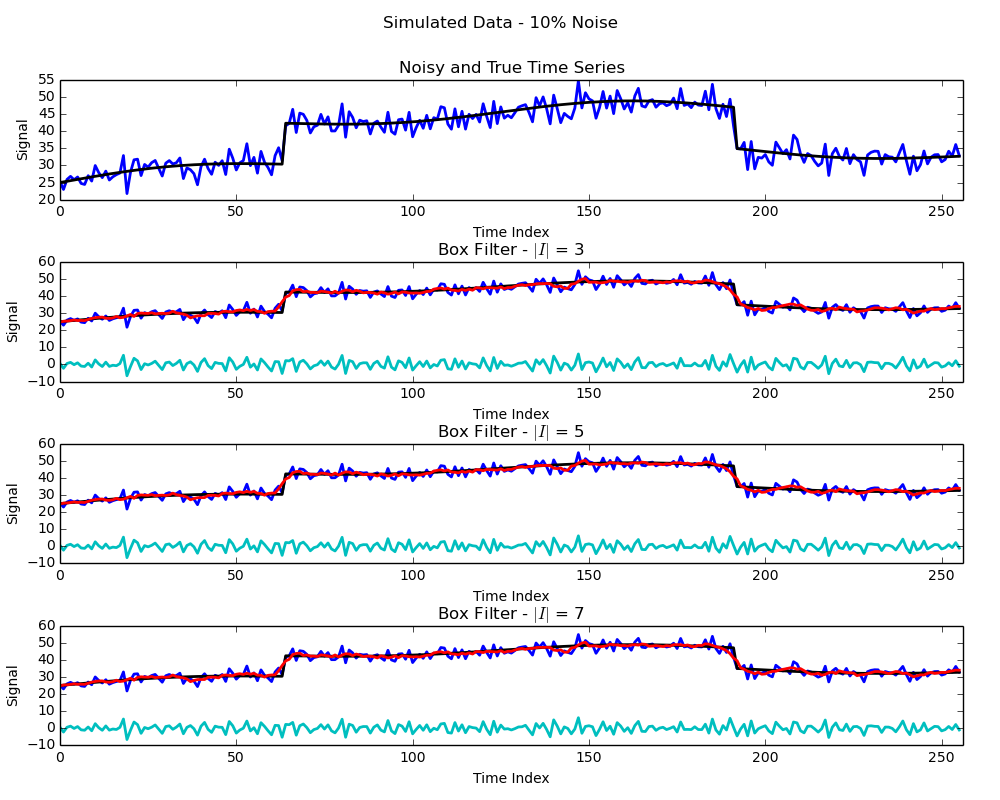
\includegraphics[width = 0.75 \textwidth]{BoxCompare.png}
\caption{Box Filter with simulated data}
\label{boxcompare}
\end{figure}

The Gaussian filter is a weighted moving average that weights points further away in the time series according to a Gaussian distribution with standard deviation $\sigma$. The smoothed values from the Gaussian filter are given by

\begin{displaymath}
s_i = \sum _{i \in I} w \left(i, j \right) y_j
\end{displaymath}

\noindent
where the weights are given by the function

\begin{displaymath}
w\left(i, j\right) = \frac{1}{z_i} \frac{1}{\sqrt{2 \pi} \sigma_d} e^{-\frac{\lvert i - j \rvert}{2 \sigma_d^2}}
\end{displaymath}

\noindent
where $z_i$ is a normalization factor.\\

Typically a interval width of $10 \sigma_d$ is used. This accounts for $99.99994\%$ of the area under the curve in a Gaussian distribution. Some computations can be saved by using an interval width of $8 \sigma_d$, $99.994\%$ of the area under the curve in a Gaussian distribution, or $6 \sigma_d$, $99.7\%$ of the area under the curve in a Gaussian distribution. In this technique, the Gaussian kernel standard deviation, $\sigma_d$, is a parameter to be chosen by the analyst. As seen in Figure \ref{gaussiancompare}, the Gaussian filter does a reasonable job removing noise but also destroys features in the time series.\\

\begin{figure}
\centering
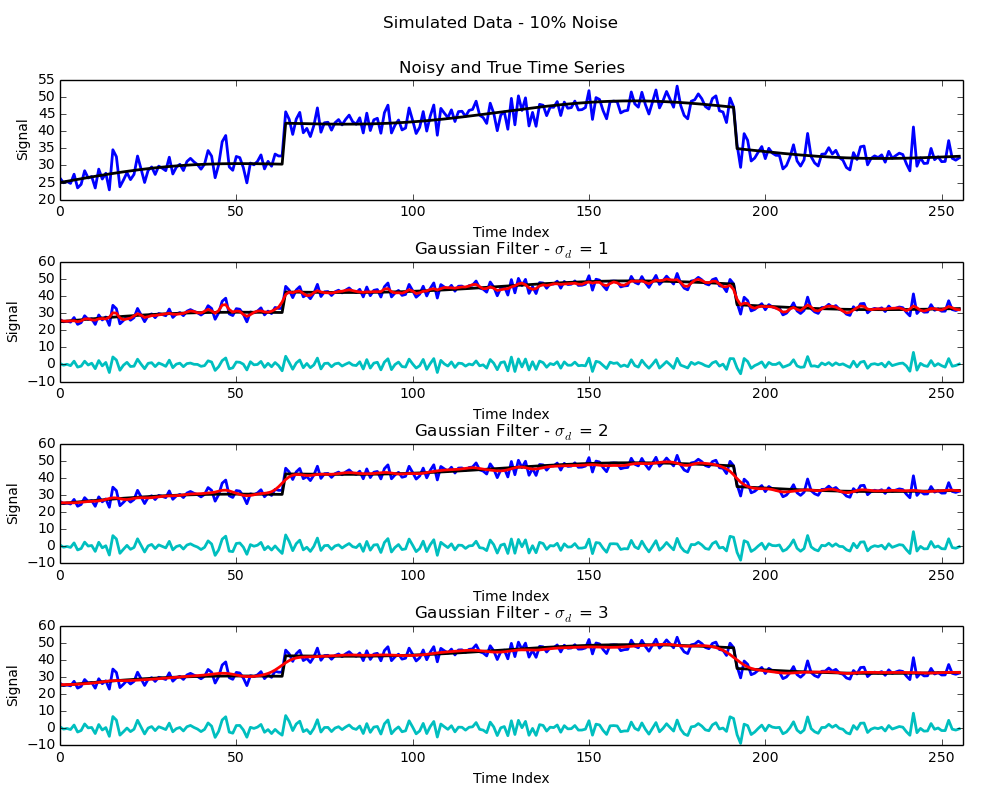
\includegraphics[width = 0.75 \textwidth]{GaussianCompare.png}
\caption{Gaussian Filter with simulated data}
\label{gaussiancompare}
\end{figure}

The Gaussian filter can still remove features of interest in the signal. The Bilateral filter attempts to help correct this by applying a pair of Gaussian weights, one for spatial distance, as in the Gaussian filter, and one for differences in intensity values. The smoothed values from the Bilateral filter are given by

\begin{displaymath}
s_i = \sum _{i \in I} w \left(i, j \right) y_j
\end{displaymath}

\noindent
where the weights are given by the function

\begin{displaymath}
w\left(i, j\right) = \frac{1}{z_i} \frac{1}{2 \pi \sigma_d \sigma_i} e^{-\frac{\lvert i - j \rvert}{2 \sigma_d^2}}e^{-\frac{\lvert y_i - y_j \rvert}{2 \sigma_i^2}}
\end{displaymath}

\noindent
where, as before, $z_i$ is a normalization factor.\\

As before, an interval width of $10 \sigma$ is typical. In this technique, the Gaussian kernel standard deviations, $\sigma_d$ and $\sigma_i$, are two parameters to be chosen by the analyst. As seen in Figure \ref{bilateralcompare}, the bilateral filter does a reasonable job both smoothing the time series and retaining features. Unfortunately, the bilateral filter may retain some of the noise, especially near large features in the time series.\\

\begin{figure}
\centering
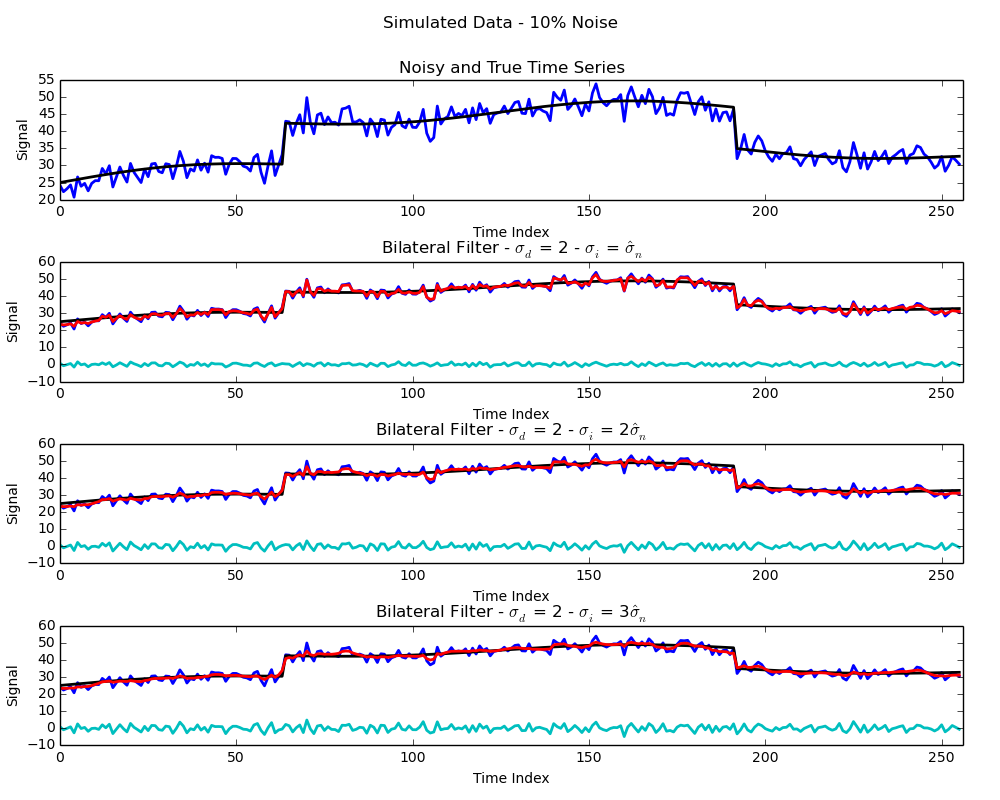
\includegraphics[width = 0.75 \textwidth]{BilateralCompare.png}
\caption{Bilateral Filter with simulated data}
\label{bilateralcompare}
\end{figure}

Zang and Gunturk~\cite{Zang08} suggest that the optimal value of the standard deviation of the spatial Gaussian kernel, $\sigma_d$, is in the range $[ 1.5, 2.1 ]$ and the standard deviation of the intensity Gaussian kernel, $\sigma_i$, is in the range $[ 1.5 \sigma_n, 3 \sigma_n ]$ for $2$D image processing. It is uncertain if these results translate to $1$D signal processing.\\

It is important to note that treatment of edge values is important, particularly when incrementally processing a time series. In the case of spatial filters, the $\frac{\lvert I \rvert - 1}{2}$ values on the edges do not have complete intervals. We adjust normalization factor $z_i$ to ensure that the weight values in the incomplete interval still sum to $1$.\\

With this edge treatment, it is simple to adjust the time series when a new data point is received. With the updated time series, the last $\frac{\lvert I \rvert - 1}{2}$ smoothed values can be updated and a new smoothed value can be calculated as before.

\newpage

\subsection{Frequency Filters}

Time series data can also be analyzed in the frequency domain. Noise might be represented as small coefficients in the frequency domain that can be eliminated with thresholding.\\

Historically, analysis in the frequency domain was conducted via the Fourier Transform in it\rq{}s rapid discrete form, the Fast Fourier Transform (FFT). The FFT takes uniformly spaced observations and can transform the data with an order of $n$ log $n$ operations. After transformation, coefficient thresholding is used on the signal frequency coefficients to denoise the data, and then the denoised frequency coefficients are reverse transformed. As can be seen in Figure \ref{fftcompare}, the Fourier Transform struggles near the edges, where Gibbs phenomenon may occur. this makes the Fourier Transform less than ideal for incremental data denoising, where the most relevant data is near the end of the time series.\\

\begin{figure}
\centering
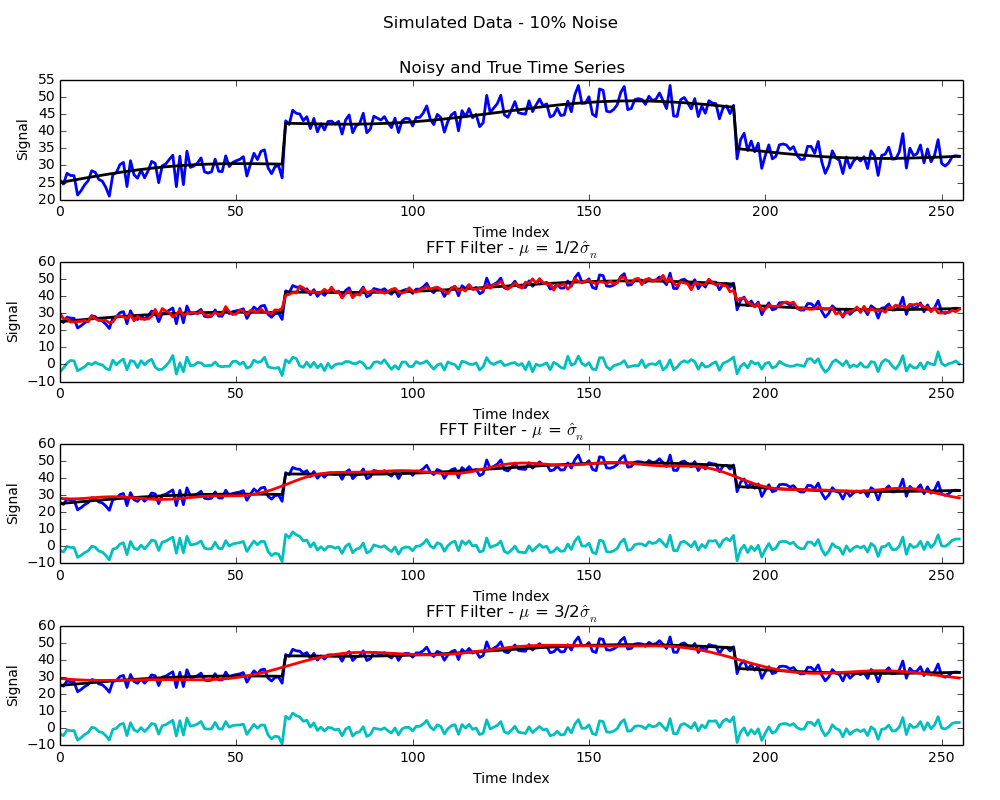
\includegraphics[width = 0.75 \textwidth]{FFTCompare.png}
\caption{Fourier Transform Filter with simulated data}
\label{fftcompare}
\end{figure}

The wavelet transform is one of the most popular alternatives to the Fourier transform. While the Fourier transform completely transforms the time series into the frequency domain, the wavelet transform offers both frequency and time information. This allows for filtering both by frequency and temporal relationships~\cite{Graps95}. There are a variety of wavelet families to choose from, and the wavelet transformations can be repeated to a desired level of resolution. We have used the Harr wavelet, but many other families of wavlets give better performance.\\

Mota, Vasconcelos, and Silva~\cite{Mota05} outlined a algorithm for processing continuous data streams in real time using the discrete wavelet transform, inspired by an older result by Vishwanath, called the Recursive Pyramid Algorithm~\cite{Vishwanath94}. For the purposes of incremental data processing, these algorithms may be unnecessary if the time between data points is large enough.\\

There are two common procedures for modifying noisy frequency coefficients for Fourier or wavelet transformed data, known as thresholding methods (Donoho and Johnstone~\cite{Donoho94}). The first, \textit{hard thresholding}, cancels all coefficients smaller than a particular threshold. $v\left(\alpha\right)$ represents the transformed data, the frequency coefficients.

\begin{displaymath}
v\left(\alpha\right) = 
\begin{cases}
v\left(\alpha\right) & \lvert v\left(\alpha\right)\rvert > \mu \\
0 & \lvert v\left(\alpha\right)\rvert < \mu
\end{cases}
\end{displaymath}

Hard thresholding can create wavelet outliers, which can be partially avoided using \textit{soft thresholding}.

\begin{displaymath}
v\left(\alpha\right) = 
\begin{cases}
v\left(\alpha\right) - sgn\left(v\left(\alpha\right)\right)\mu & \lvert v\left(\alpha\right)\rvert \geq \mu \\
0 & \lvert v\left(\alpha\right)\rvert < \mu
\end{cases}
\end{displaymath}

Unfortunately, soft thresholding can create problems with the scale of the reverse transformed data which can make it inappropriate for time series were the scale of the data is important. For this reason, we will only consider hard thresholding.\\

The theoretically optimal threshold is $\mu = \sigma \sqrt{2 log I}$, where $I$ is the number of data points and $\sigma$ is the standard deviation of the coefficients. In order to avoid inflating the standard deviation of the coefficients through a large coefficient corresponding to the mean of the data, the mean is subtracted from the time series prior to transformation, making the time series a zero-mean dataset. In practice this threshold is too high and cancels too many coefficients that do not correspond to noise. In practice $\mu = 3 \sigma$ is used for hard thresholding and $\mu = \frac{3}{2} \sigma$ is used for soft thresholding~\cite{Buades05}. It is uncertain if these results translate to $1$D signal processing.\\

In this algorithm, the analyst can control the choice of wavelet, the number of levels, and the thresholding cutoff, $\mu$. Figure \ref{waveletcompare} shows the results from denoising with a Harr wavelet transform, with different hard thresholds.\\

\begin{figure}
\centering
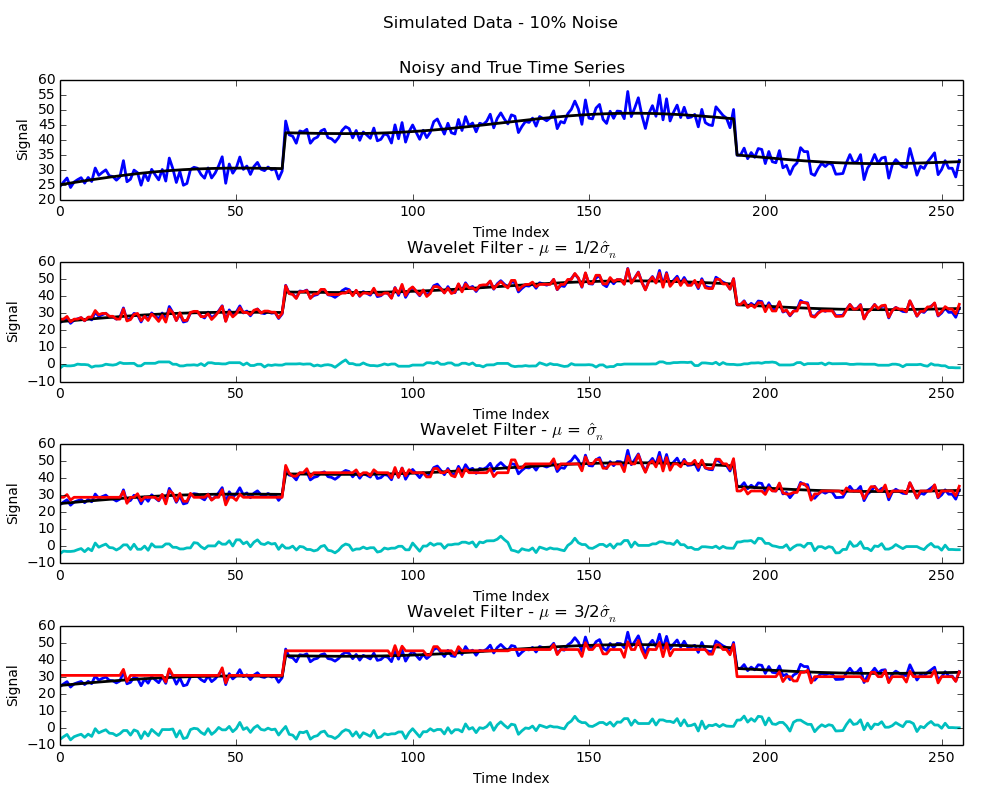
\includegraphics[width = 0.75 \textwidth]{WaveletCompare.png}
\caption{Wavelet Transform Filter with simulated data}
\label{waveletcompare}
\end{figure}

In this case, there is no special edge treatment. Incremental data processing can be accomplished via a real time algorithm, as mentioned above, or it could be accomplished by rerunning the transformation, thresholding, and back transformation on a sufficient number of the most recent data points to ensure enough coefficients at the desired level.

\newpage

\subsection{Statistical Neighborhood Filters}

Statistical neighborhood filters attempt to fix the problems associated with local smoothing filters by calculating the smoothed value as a weighted average of other values in the time series upon the similarity between the neighborhoods around the time series values. The non-local means algorithm was first introduced by Buades et al.~\cite{Buades05}. Non-local means has primarily been used for image processing, but it has been mentioned in a $1$D context in several papers (~\cite{Galiano13}, ~\cite{Tracey12}, ~\cite{Zoican10}).  We will investigate a modification of this algorithm by for efficient $3$D medical image processing by Coup{\'e} et al.~\cite{Coupe07}.\\

In the non-local means algorithm, smoothed values are given by

\begin{displaymath}
s_i = \sum _{i \in N} w \left(i, j \right) y_j
\end{displaymath}

\noindent
where the weights are given by the function

\begin{displaymath}
w \left(i, j \right) = \frac{1}{z_i} e^{-\frac{\lvert Y_i - Y_j \rvert ^2}{2 \beta \hat{\sigma}^2_n \lvert Y \rvert}}
\end{displaymath}

In this scheme, $Y_i$ is a vector of intensity values in the interval, or neighborhood, around $y_i$, $\lvert Y_i - Y_j \rvert$ is the $L_2$ norm of the difference in intensity values in these intervals, $\lvert Y \rvert$ is the window size, and $\beta$ is a parameter chosen by the analyst to control the amount of smoothing. According to Coup{\'e} et al.~\cite{Coupe07}, $\beta$ varies between $0$ and $1$, with values of $\beta$ closer to $1$ better for high levels of noise and values of $\beta$ closer to $0.5$ better for lower levels of noise.\\

Duval et al.~\cite{Duval11} notes that neighborhood preselection can improve the results of the non-local means algorithm by assigning a weight of $0$ to the $y_j$ values that have neighborhoods that are too dissimilar from the $Y_i$ under consideration. Duval et al. uses a preslection test based upon the norm of the difference between windows. A more complex preselection method is described by Buades et al.~\cite{Buades05}. We use Duval et al.'s  preselection test:

\begin{displaymath}
w\left(i, j\right) = 
\begin{cases}
\frac{1}{z_i} e^{-\frac{\lvert Y_i - Y_j \rvert ^2}{2 \beta \hat{\sigma}^2_n \lvert Y \rvert}} & \lvert Y_i - Y_j \rvert < T \\
0 & $otherwise$
\end{cases}
\end{displaymath}

Duval et al.~\cite{Duval11} suggests that values of $T$ near $20$ or $30$ work well for $2$D images. This type of threshold does not work well for signal analysis. We will consider thresholds of the type $T = \left( max Y_j - min Y_j \right) \lvert I \rvert \delta$, where $\delta \in \left[ 0, 1 \right]$. Duval et al. recommends that window sizes of $5$ or $7$ are appropriate for $2$D image processing. As before, it is uncertain if these results translate to $1$D signal processing.\\

In this algorithm, the analyst can control the amount of smoothing via $\beta$, the preselection parameter $\delta$, the interval size, and the search window size. Figure \ref{nlmeanscompare} shows the performance of the Non-Local Means technique with different values of $\beta$. For this figure, $\mu_1 = 0.95$, $\sigma_1 = 0.5$, and $\lvert I \rvert = 7$. Notice how similar the performance is to the bilateral filter, Figure \ref{bilateralcompare}.\\

\begin{figure}
\centering
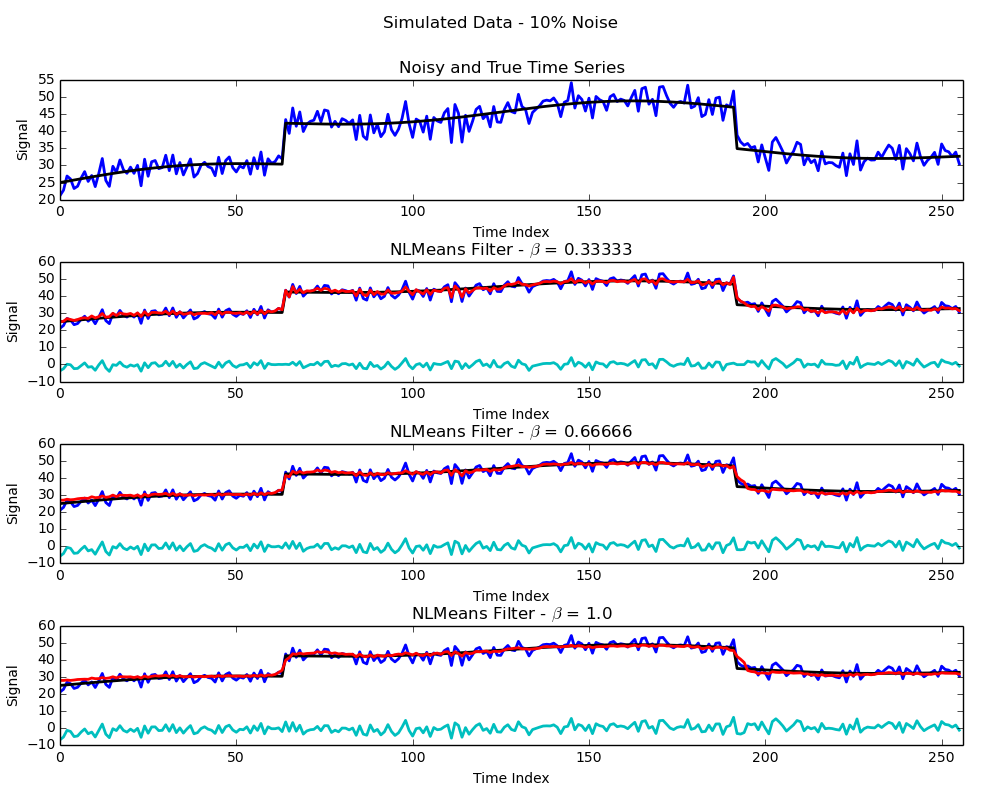
\includegraphics[width = 0.75 \textwidth]{NLMeansCompare.png}
\caption{Non-Local Means Filter with simulated data}
\label{nlmeanscompare}
\end{figure}

As with the spatial filters, the $\frac{\lvert I \rvert - 1}{2}$ values on the edges do not have complete intervals. In order to calculate weights, we compare the incomplete neighborhood $Y_i$ with incomplete neighborhoods around the other points $Y_j$. We adjust normalization factor $z_i$ to ensure that the weight values in the incomplete interval still sum to $1$.\\

With this edge treatment, it is simple to adjust the time series when a new data point is received. With the updated time series, the last $\frac{\lvert I \rvert - 1}{2}$ smoothed values can be updated and a new smoothed value can be calculated as before.

\newpage

\subsection{Combination Techniques}

There are a variety of ways to combine or iterate techniques.\\

Iterating the box filter and Gaussian filter is well understood and is equivalent to using a box filter or Gaussian filter with a wider window or $\sigma_d$. We will not investigate these here. Iterating the Fourier Transform or Wavelet Transform filtering is equivalent to using a Fourier Transform or Wavelet Transform filter with a higher frequency coefficient threshold. We will not investigate these here either.\\

Iterating a Bilateral filter or Non-Local Means filter is more complex. Also, the question of combining a Bilateral filter and Non-Local Means filter is open. We will investigate all three of these possibilities.


\section{Parameter Optimization}


\section{Comparison}

In this section we will the results of the denoising techniques for time series. We will consider both known time series with added noise and real world time series. First we will consider optimal choices for the standpoint of peak signal to noise ratio (PSNR) with known time series with added noise. We will consider AWGN, blah, and blah. Next, we will compare the automatic parameter optimization techniques to the results from PSNR. Finally, we will consider the results from automatic parameter optimization on real world time series.

\subsection{Known Time Series with Noise Added - Parameter Evaluation with PSNR}

In this section we will consider the performance of denoising algorithms on known time series with added noise. We will assess the selected parameters with PSNR.\\

PSNR, peak signal to noise ratio, is a measure of how effective the denoising algorithm was. It is calculated as follows:

\begin{displaymath}
PSNR = 10 log_{10} \left( \frac{max _{i \in \Omega} ^2 \left( y_i \right)}{MSE} \right)
\end{displaymath}

where $MSE$, mean square error, is

\begin{displaymath}
MSE = \frac{1}{N} \sum _{i = 0} ^{N - 1} \left( y_i - s_i \right) ^2
\end{displaymath}

It is important to note that PSNR is one of the most popular, but not the only measure of quality for a denoised time series. PSNR is a global measure of quality, where higher values indicate a less noisy signal. We will look for denoising methods that are relatively insensitive to parameter choice within an optimal range.\\

We are assessing the performance of the denoising algorithms with three known time series with $1$, $5$, $10$, $20$, and $30$ percent added noise, Figures \ref{signal1compare}, \ref{signal2compare}, and \ref{signal3compare}. Noise of a particular percentage is added by using $v p$ as the standard deviation of the distribution that generated the noise, were $v$ is the maximum possible range of values that the time series could take and $p$ is the percentage.\\

\begin{figure}
\centering
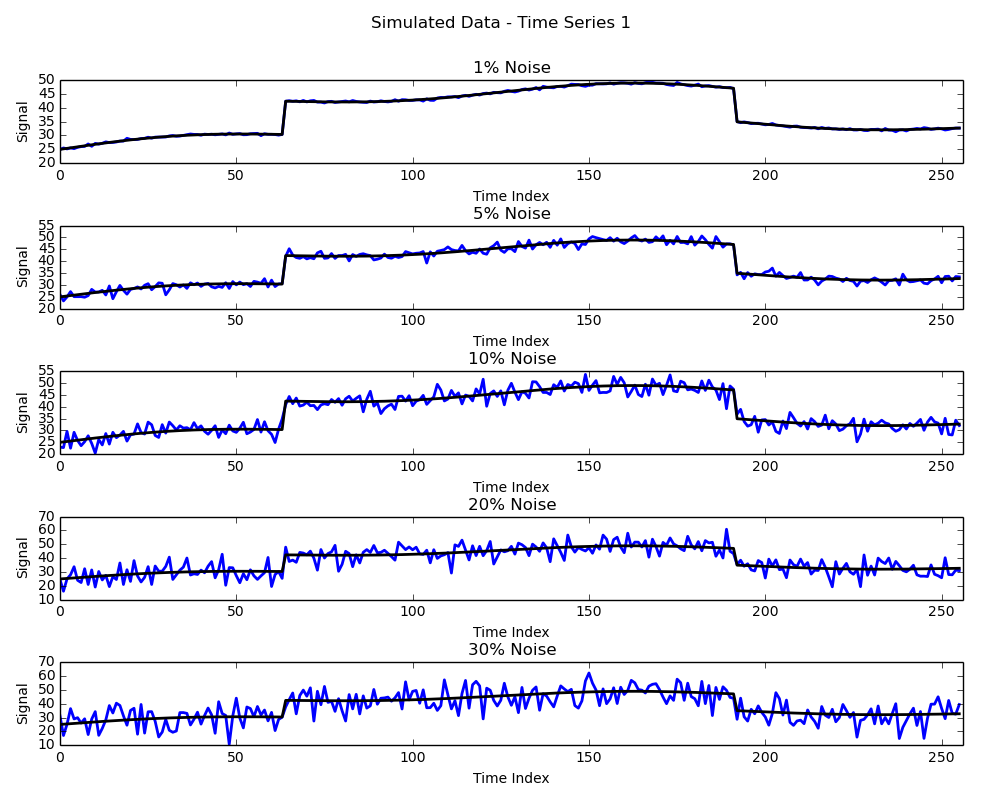
\includegraphics[width = 0.75 \textwidth]{Signal1Compare.png}
\caption{Time Series 1}
\label{signal1compare}
\end{figure}

\begin{figure}
\centering
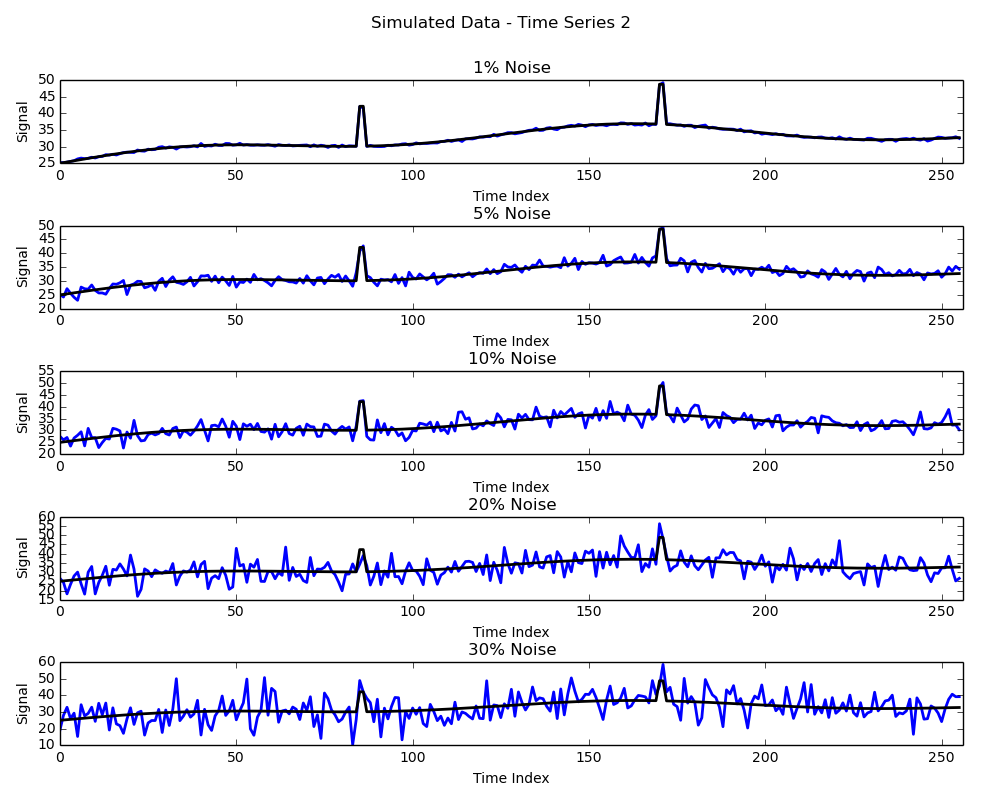
\includegraphics[width = 0.75 \textwidth]{Signal2Compare.png}
\caption{Time Series 2}
\label{signal2compare}
\end{figure}

\begin{figure}
\centering
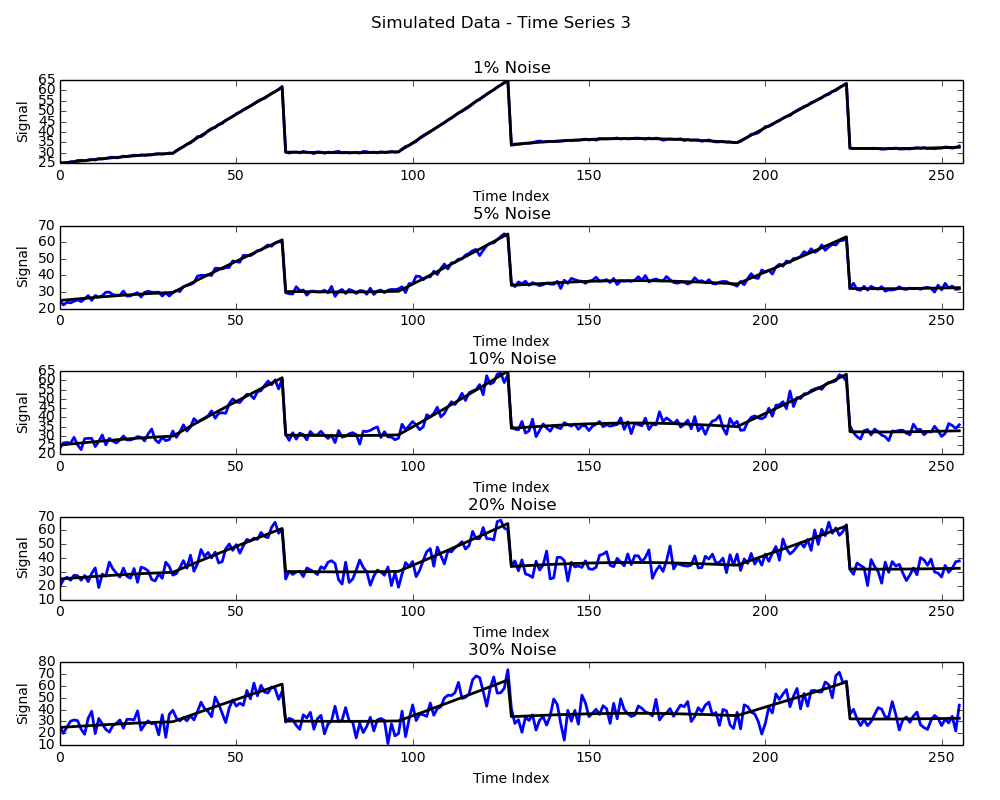
\includegraphics[width = 0.75 \textwidth]{Signal3Compare.png}
\caption{Time Series 3}
\label{signal3compare}
\end{figure}

All of the time series were created by taking low frequency sinusoidal behavior and adding features of interest. There are a few interesting observations that can be made about the three time series.\\

The first time series, Figure \ref{signal1compare}, was created by taking low frequency sinusoidal behavior and adding a sharp increase in intensity one quarter of the way through the time series and adding a sharp decrease in intensity three quarters of the way through the time series. In some cases the noise obscures the sharp increase or decrease in intensity, making it appear to be a more gradual increase or decrease in intensity. Noise can make features impossible to recover.\\

The second time series, Figure \ref{signal2compare}, was created by taking low frequency sinusoidal behavior and adding two brief, sharp increases in intensity, at one and two thirds of the way through the time series. In some cases the noise can become indistinguishable from these features, making them impossible to recover.\\

The third time series, Figure \ref{signal3compare}, was created by taking low frequency sinusoidal behavior and adding three sawtooth features, at one, three, and six eights of the way through the time series. As with the first time series, it is possible for the noise to obscure the sharp decrease at the end of the saw tooth features, making it appear to be a more gradual decrease in intensity.\\

These denoising techniques were assessed in a full factorial design over the following parameter ranges:

\begin{enumerate}

\item Nose: $1$\%, $5$\%, $10$\%, $20$\%, and $30$\%

\item $\lvert I \rvert$: $3$, $5$, $7$, and $9$

\item $\sigma_d$: $0.1$, $1.0$, $2.0$, $3.0$, and $4.0$

\item $\sigma_i$: $0.1 \hat{\sigma}_n$, $1.0 \hat{\sigma}_n$, $2.0 \hat{\sigma}_n$, $3.0 \hat{\sigma}_n$,  and $4.0 \hat{\sigma}_n$

\item $\mu$: $0.1 \sigma$, $1.0 \sigma$, $2.0 \sigma$, and $3.0 \sigma$

\item $\beta$: $0.5$, $0.75$, and $1.0$

\item $T$: $0.25 \left( max Y_j - min Y_j \right) \lvert I \rvert$, $0.5 \left( max Y_j - min Y_j \right) \lvert I \rvert$, and $0.75 \left( max Y_j - min Y_j \right) \lvert I \rvert$

\end{enumerate}

$5$ iterations were run at each combination of parameters for each denoising method. Further iterations were run at a finer resolution at parameter values that appeared to be near optimal for each denoising method. For each iteration, a new noisy signal was created, denoised, and then PSNR was calculated. An ordinary least squares optimization was then used to fit a quadratic model with interactions to the results. The model and findings for each denoising technique are listed below. 

\subsubsection{Box Filter}

The regression models are shown below, in Listings \ref{boxfilterseries1}, \ref{boxfilterseries2}, and \ref{boxfilterseries3}. The regression models seem to indicate that that the level of added noise is the only significant indicator for the quality of the denoised signal. The one parameter in the box filter, the window size, has no consistent, significant impact on the PSNR of the denoised signal. This highlights why the box filter is not in common usage in time series denoising.\\

Figures \ref{box1best}, \ref{box2best}, and \ref{box3best} show the best performance of the Box filter for each time series.

{\footnotesize
\begin{lstlisting}[caption = Time Series 1 - Box Filter OLS Model, label = {boxfilterseries1}]
                            OLS Regression Results                            
==============================================================================
Dep. Variable:                   PSNR   R-squared:                       0.972
Model:                            OLS   Adj. R-squared:                  0.971
Method:                 Least Squares   F-statistic:                     1105.
Date:                Thu, 03 Jul 2014   Prob (F-statistic):           2.88e-74
Time:                        10:36:38   Log-Likelihood:                -202.54
No. Observations:                 100   AIC:                             413.1
Df Residuals:                      96   BIC:                             423.5
Df Model:                           3                                         
==================================================================================
                     coef    std err          t      P>|t|      [95.0% Conf. Int.]
----------------------------------------------------------------------------------
Intercept         84.5463      1.564     54.054      0.000        81.442    87.651
Noise             -1.0227      0.018    -57.556      0.000        -1.058    -0.987
Window             0.5020      0.568      0.884      0.379        -0.625     1.629
I(Window ** 2)    -0.0504      0.047     -1.077      0.284        -0.143     0.043
==============================================================================
Omnibus:                        0.962   Durbin-Watson:                   0.974
Prob(Omnibus):                  0.618   Jarque-Bera (JB):                0.628
Skew:                          -0.185   Prob(JB):                        0.731
Kurtosis:                       3.118   Cond. No.                         451.
==============================================================================
\end{lstlisting}

\begin{lstlisting}[caption = Time Series 2 - Box Filter OLS Model, label = {boxfilterseries2}]
                            OLS Regression Results                            
==============================================================================
Dep. Variable:                   PSNR   R-squared:                       0.977
Model:                            OLS   Adj. R-squared:                  0.977
Method:                 Least Squares   F-statistic:                     1380.
Date:                Thu, 03 Jul 2014   Prob (F-statistic):           8.74e-79
Time:                        10:40:12   Log-Likelihood:                -158.53
No. Observations:                 100   AIC:                             325.1
Df Residuals:                      96   BIC:                             335.5
Df Model:                           3                                         
==================================================================================
                     coef    std err          t      P>|t|      [95.0% Conf. Int.]
----------------------------------------------------------------------------------
Intercept         71.9697      1.007     71.448      0.000        69.970    73.969
Noise             -0.7361      0.011    -64.329      0.000        -0.759    -0.713
Window             0.4161      0.366      1.138      0.258        -0.310     1.142
I(Window ** 2)    -0.0285      0.030     -0.947      0.346        -0.088     0.031
==============================================================================
Omnibus:                       16.755   Durbin-Watson:                   1.879
Prob(Omnibus):                  0.000   Jarque-Bera (JB):               29.075
Skew:                           0.688   Prob(JB):                     4.86e-07
Kurtosis:                       5.255   Cond. No.                         451.
==============================================================================
\end{lstlisting}

\begin{lstlisting}[caption = Time Series 3 - Box Filter OLS Model, label = {boxfilterseries3}]
                            OLS Regression Results                            
==============================================================================
Dep. Variable:                   PSNR   R-squared:                       0.948
Model:                            OLS   Adj. R-squared:                  0.947
Method:                 Least Squares   F-statistic:                     829.3
Date:                Thu, 03 Jul 2014   Prob (F-statistic):           3.57e-87
Time:                        10:42:53   Log-Likelihood:                -185.21
No. Observations:                 140   AIC:                             378.4
Df Residuals:                     136   BIC:                             390.2
Df Model:                           3                                         
==================================================================================
                     coef    std err          t      P>|t|      [95.0% Conf. Int.]
----------------------------------------------------------------------------------
Intercept         68.3722      0.649    105.429      0.000        67.090    69.655
Noise             -0.3854      0.008    -49.876      0.000        -0.401    -0.370
Window            -0.0358      0.236     -0.152      0.880        -0.503     0.431
I(Window ** 2)     0.0041      0.019      0.211      0.833        -0.034     0.043
==============================================================================
Omnibus:                        7.975   Durbin-Watson:                   1.624
Prob(Omnibus):                  0.019   Jarque-Bera (JB):               14.313
Skew:                          -0.149   Prob(JB):                     0.000780
Kurtosis:                       4.538   Cond. No.                         445.
==============================================================================
\end{lstlisting}
}

\begin{figure}
\centering
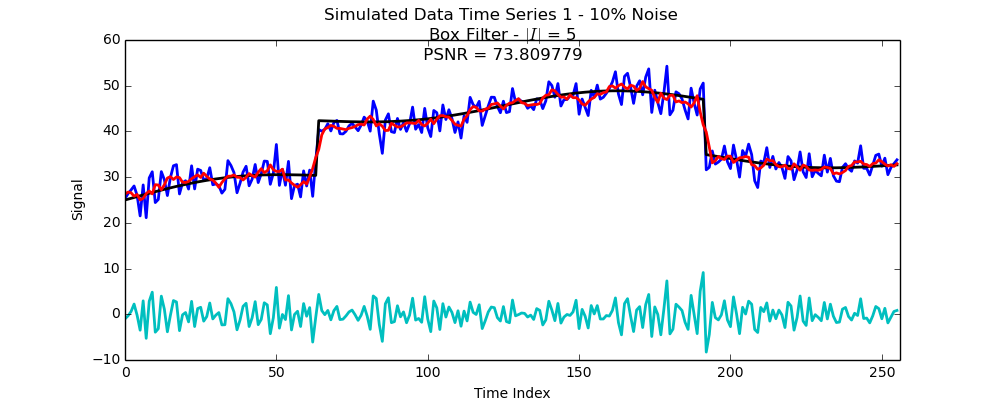
\includegraphics[width = 0.75 \textwidth]{BoxSignal1Best.png}
\caption{Box Filter - Best Denosing with 10\% Noise - Time Series 1}
\label{box1best}
\end{figure}

\begin{figure}
\centering
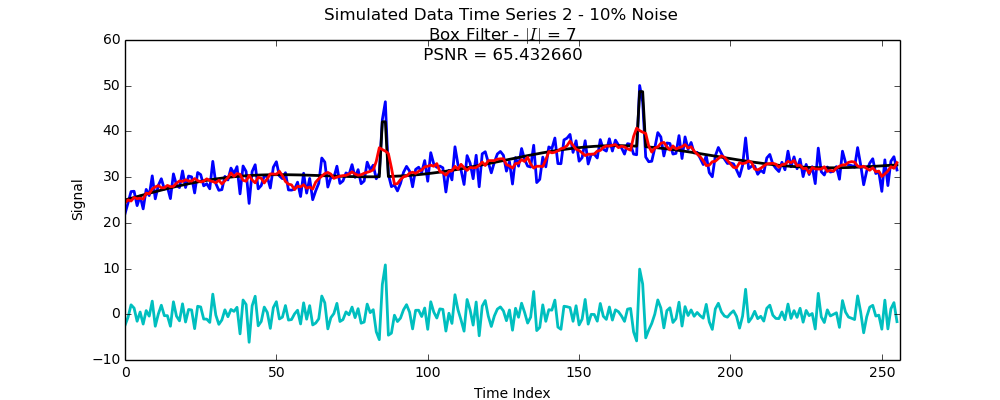
\includegraphics[width = 0.75 \textwidth]{BoxSignal2Best.png}
\caption{Box Filter - Best Denosing with 10\% Noise - Time Series 2}
\label{box2best}
\end{figure}

\begin{figure}
\centering
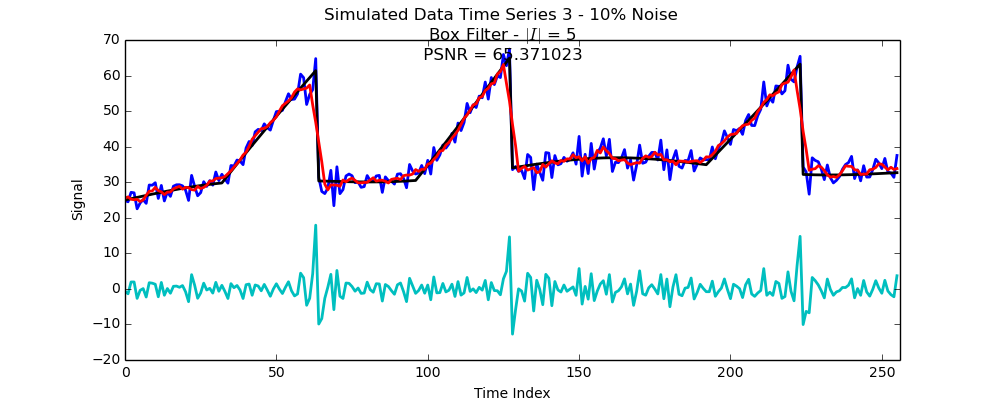
\includegraphics[width = 0.75 \textwidth]{BoxSignal3Best.png}
\caption{Box Filter - Best Denosing with 10\% Noise - Time Series 3}
\label{box3best}
\end{figure}

\newpage

\subsubsection{Gaussian Filter}

The regression models are shown below, in Listings \ref{gaussianfilterseries1}, \ref{gaussianfilterseries2}, and \ref{gaussianfilterseries3}. For time series 1 and 2, optimal values of $\sigma_d$ appear to be in the range $\left[ 1.5, 3.0 \right]$. The optimal value of $\sigma_d$ for time series 3 seems to be inconsistent with the results from time series 1 and 2, but this could be a function of the fact that time series 3 has more jump discontinuities, which we would expect the Gaussian filter to have difficulty with. It is also interesting to note that larger values of $\sigma_d$ are needed with larger levels of noise.\\

Figures \ref{gaussian1best}, \ref{gaussian2best}, and \ref{gaussian3best} show the best performance of the Gaussian filter for each time series.

{\footnotesize
\begin{lstlisting}[caption = Time Series 1 - Gaussian Filter OLS Model, label = {gaussianfilterseries1}]
                            OLS Regression Results                            
==============================================================================
Dep. Variable:                   PSNR   R-squared:                       0.966
Model:                            OLS   Adj. R-squared:                  0.965
Method:                 Least Squares   F-statistic:                     1020.
Date:                Thu, 03 Jul 2014   Prob (F-statistic):          4.85e-105
Time:                        10:49:35   Log-Likelihood:                -303.91
No. Observations:                 150   AIC:                             617.8
Df Residuals:                     145   BIC:                             632.9
Df Model:                           4                                         
================================================================================
                   coef    std err          t      P>|t|      [95.0% Conf. Int.]
--------------------------------------------------------------------------------
Intercept       72.4305      1.016     71.319      0.000        70.423    74.438
Noise           -1.0206      0.045    -22.870      0.000        -1.109    -0.932
SigD             8.3538      0.578     14.453      0.000         7.211     9.496
Noise:SigD       0.1071      0.018      5.975      0.000         0.072     0.142
I(SigD ** 2)    -1.6241      0.112    -14.538      0.000        -1.845    -1.403
==============================================================================
Omnibus:                        0.512   Durbin-Watson:                   1.662
Prob(Omnibus):                  0.774   Jarque-Bera (JB):                0.229
Skew:                           0.059   Prob(JB):                        0.892
Kurtosis:                       3.150   Cond. No.                         384.
==============================================================================
\end{lstlisting}

\begin{lstlisting}[caption = Time Series 2 - Gaussian Filter OLS Model, label = {gaussianfilterseries2}]
                            OLS Regression Results                            
==============================================================================
Dep. Variable:                   PSNR   R-squared:                       0.943
Model:                            OLS   Adj. R-squared:                  0.942
Method:                 Least Squares   F-statistic:                     603.3
Date:                Thu, 03 Jul 2014   Prob (F-statistic):           2.93e-89
Time:                        10:51:38   Log-Likelihood:                -301.77
No. Observations:                 150   AIC:                             613.5
Df Residuals:                     145   BIC:                             628.6
Df Model:                           4                                         
================================================================================
                   coef    std err          t      P>|t|      [95.0% Conf. Int.]
--------------------------------------------------------------------------------
Intercept       69.4749      1.001     69.393      0.000        67.496    71.454
Noise           -0.9668      0.044    -21.975      0.000        -1.054    -0.880
SigD             4.2372      0.570      7.436      0.000         3.111     5.363
Noise:SigD       0.1559      0.018      8.828      0.000         0.121     0.191
I(SigD ** 2)    -1.1943      0.110    -10.845      0.000        -1.412    -0.977
==============================================================================
Omnibus:                        2.623   Durbin-Watson:                   1.168
Prob(Omnibus):                  0.269   Jarque-Bera (JB):                2.256
Skew:                           0.173   Prob(JB):                        0.324
Kurtosis:                       3.491   Cond. No.                         384.
==============================================================================
\end{lstlisting}

\begin{lstlisting}[caption = Time Series 3 - Gaussian Filter OLS Model, label = {gaussianfilterseries3}]
                            OLS Regression Results                            
==============================================================================
Dep. Variable:                   PSNR   R-squared:                       0.750
Model:                            OLS   Adj. R-squared:                  0.745
Method:                 Least Squares   F-statistic:                     146.4
Date:                Thu, 03 Jul 2014   Prob (F-statistic):           1.36e-57
Time:                        10:53:34   Log-Likelihood:                -603.64
No. Observations:                 200   AIC:                             1217.
Df Residuals:                     195   BIC:                             1234.
Df Model:                           4                                         
================================================================================
                   coef    std err          t      P>|t|      [95.0% Conf. Int.]
--------------------------------------------------------------------------------
Intercept       91.4141      1.392     65.653      0.000        88.668    94.160
Noise           -1.4539      0.074    -19.704      0.000        -1.599    -1.308
SigD           -11.5255      1.071    -10.761      0.000       -13.638    -9.413
Noise:SigD       0.4484      0.030     15.021      0.000         0.389     0.507
I(SigD ** 2)     0.3986      0.239      1.671      0.096        -0.072     0.869
==============================================================================
Omnibus:                      124.517   Durbin-Watson:                   0.495
Prob(Omnibus):                  0.000   Jarque-Bera (JB):             1068.943
Skew:                           2.267   Prob(JB):                    7.62e-233
Kurtosis:                      13.379   Cond. No.                         211.
==============================================================================
\end{lstlisting}
}

\begin{figure}
\centering
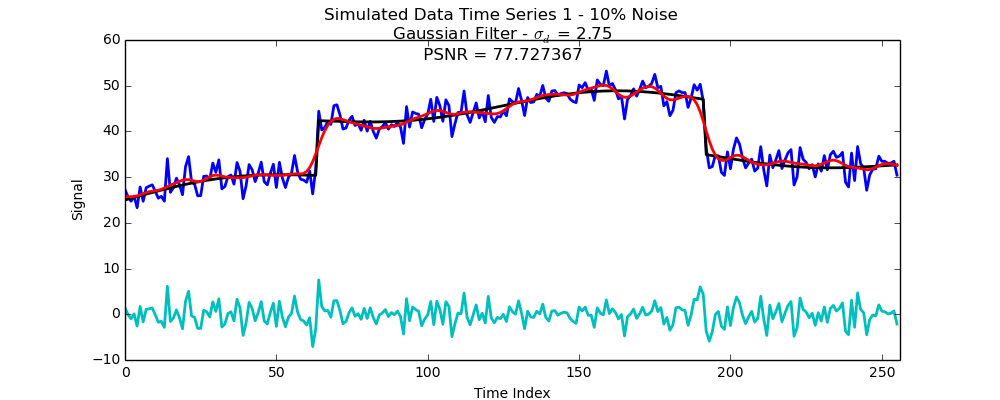
\includegraphics[width = 0.75 \textwidth]{GaussianSignal1Best.png}
\caption{Gaussian Filter - Best Denosing with 10\% Noise - Time Series 1}
\label{gaussian1best}
\end{figure}

\begin{figure}
\centering
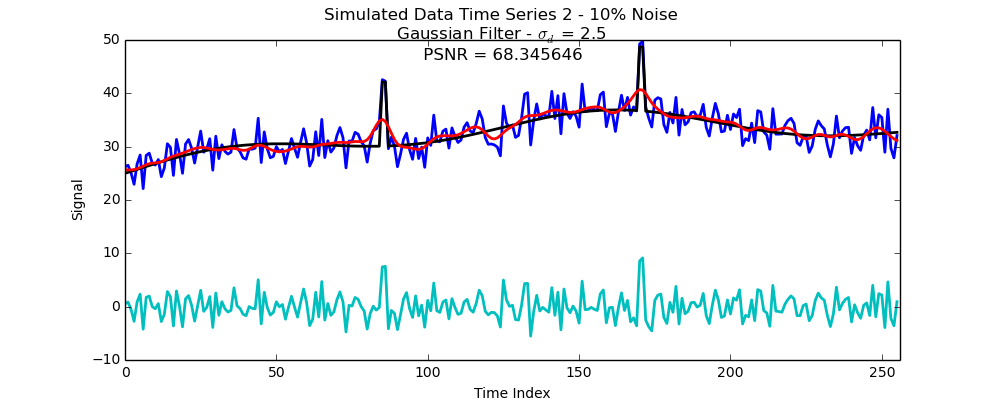
\includegraphics[width = 0.75 \textwidth]{GaussianSignal2Best.png}
\caption{Gaussian Filter - Best Denosing with 10\% Noise - Time Series 2}
\label{gaussian2best}
\end{figure}

\begin{figure}
\centering
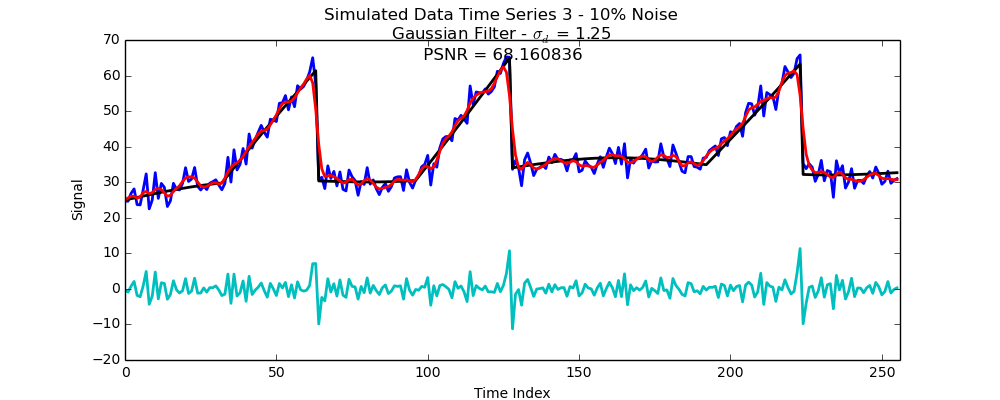
\includegraphics[width = 0.75 \textwidth]{GaussianSignal3Best.png}
\caption{Gaussian Filter - Best Denosing with 10\% Noise - Time Series 3}
\label{gaussian3best}
\end{figure}

\newpage

\subsubsection{Bilateral Filter}

The regression models are shown below, in Listings \ref{bilateralfilterseries1}, \ref{bilateralfilterseries2}, and \ref{bilateralfilterseries3}. For these signals, it appears that optimal values of $\sigma_d$ are in the range $\left[ 2.0, 3.0 \right]$ and optimal values of $\sigma_i$ are in the range $\left[ 2.0 \hat{\sigma}_n, 3.0 \hat{\sigma}_n \right]$. There is some interaction between $\sigma_d$ and $\sigma_i$ for time series 1 and 2, but not time series 3. There is not interaction between $\sigma_d$ or $\sigma_i$ and the amount of noise in the time series.\\

Figures \ref{bilateral1best}, \ref{bilateral2best}, and \ref{bilateral3best} show the best performance of the Bilateral filter for each time series.

{\footnotesize
\begin{lstlisting}[caption = Time Series 1 - Bilateral Filter OLS Model, label = {bilateralfilterseries1}]
                            OLS Regression Results                            
==============================================================================
Dep. Variable:                   PSNR   R-squared:                       0.800
Model:                            OLS   Adj. R-squared:                  0.798
Method:                 Least Squares   F-statistic:                     484.0
Date:                Thu, 03 Jul 2014   Prob (F-statistic):          3.58e-250
Time:                        10:59:15   Log-Likelihood:                -2618.8
No. Observations:                 735   AIC:                             5252.
Df Residuals:                     728   BIC:                             5284.
Df Model:                           6                                         
================================================================================
                   coef    std err          t      P>|t|      [95.0% Conf. Int.]
--------------------------------------------------------------------------------
Intercept       75.0220      1.724     43.524      0.000        71.638    78.406
Noise           -1.5113      0.034    -44.710      0.000        -1.578    -1.445
SigD             7.5535      1.132      6.670      0.000         5.330     9.777
SigI             8.0615      1.132      7.119      0.000         5.838    10.285
SigD:SigI        1.2764      0.229      5.563      0.000         0.826     1.727
I(SigD ** 2)    -1.6651      0.243     -6.866      0.000        -2.141    -1.189
I(SigI ** 2)    -1.7370      0.243     -7.162      0.000        -2.213    -1.261
==============================================================================
Omnibus:                      270.315   Durbin-Watson:                   0.125
Prob(Omnibus):                  0.000   Jarque-Bera (JB):              819.625
Skew:                           1.833   Prob(JB):                    1.05e-178
Kurtosis:                       6.650   Cond. No.                         141.
==============================================================================
\end{lstlisting}

\begin{lstlisting}[caption = Time Series 2 - Bilateral Filter OLS Model, label = {bilateralfilterseries2}]
                            OLS Regression Results                            
==============================================================================
Dep. Variable:                   PSNR   R-squared:                       0.784
Model:                            OLS   Adj. R-squared:                  0.782
Method:                 Least Squares   F-statistic:                     440.7
Date:                Thu, 03 Jul 2014   Prob (F-statistic):          1.89e-238
Time:                        11:03:34   Log-Likelihood:                -2681.4
No. Observations:                 735   AIC:                             5377.
Df Residuals:                     728   BIC:                             5409.
Df Model:                           6                                         
================================================================================
                   coef    std err          t      P>|t|      [95.0% Conf. Int.]
--------------------------------------------------------------------------------
Intercept       74.6542      1.877     39.776      0.000        70.969    78.339
Noise           -1.6212      0.037    -44.047      0.000        -1.693    -1.549
SigD             7.9290      1.233      6.431      0.000         5.508    10.350
SigI             8.6608      1.233      7.024      0.000         6.240    11.081
SigD:SigI        0.9745      0.250      3.900      0.000         0.484     1.465
I(SigD ** 2)    -1.7361      0.264     -6.574      0.000        -2.255    -1.218
I(SigI ** 2)    -1.9145      0.264     -7.250      0.000        -2.433    -1.396
==============================================================================
Omnibus:                      231.079   Durbin-Watson:                   0.146
Prob(Omnibus):                  0.000   Jarque-Bera (JB):              591.206
Skew:                           1.629   Prob(JB):                    4.18e-129
Kurtosis:                       5.948   Cond. No.                         141.
==============================================================================
\end{lstlisting}

\begin{lstlisting}[caption = Time Series 3 - Bilateral Filter OLS Model, label = {bilateralfilterseries3}]
                            OLS Regression Results                            
==============================================================================
Dep. Variable:                   PSNR   R-squared:                       0.845
Model:                            OLS   Adj. R-squared:                  0.844
Method:                 Least Squares   F-statistic:                     916.7
Date:                Thu, 03 Jul 2014   Prob (F-statistic):               0.00
Time:                        11:07:25   Log-Likelihood:                -3009.0
No. Observations:                 850   AIC:                             6030.
Df Residuals:                     844   BIC:                             6058.
Df Model:                           5                                         
================================================================================
                   coef    std err          t      P>|t|      [95.0% Conf. Int.]
--------------------------------------------------------------------------------
Intercept       89.2342      1.007     88.599      0.000        87.257    91.211
Noise           -1.7958      0.027    -65.896      0.000        -1.849    -1.742
SigD             7.2288      0.807      8.961      0.000         5.645     8.812
SigI             6.4010      0.807      7.935      0.000         4.818     7.984
I(SigD ** 2)    -1.4377      0.192     -7.507      0.000        -1.814    -1.062
I(SigI ** 2)    -1.1147      0.192     -5.820      0.000        -1.491    -0.739
==============================================================================
Omnibus:                       66.225   Durbin-Watson:                   0.102
Prob(Omnibus):                  0.000   Jarque-Bera (JB):               80.548
Skew:                           0.751   Prob(JB):                     3.23e-18
Kurtosis:                       3.127   Cond. No.                         75.6
==============================================================================
\end{lstlisting}
}

\begin{figure}
\centering
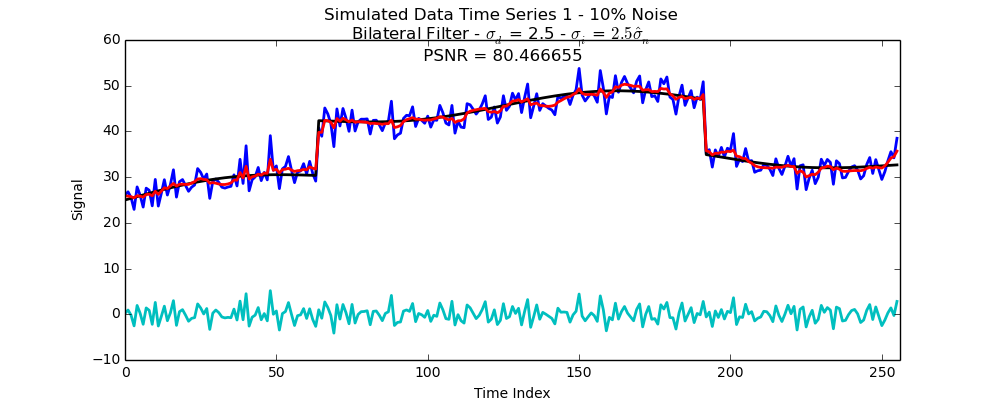
\includegraphics[width = 0.75 \textwidth]{BilateralSignal1Best.png}
\caption{Bilateral Filter - Best Denosing with 10\% Noise - Time Series 1}
\label{bilateral1best}
\end{figure}

\begin{figure}
\centering
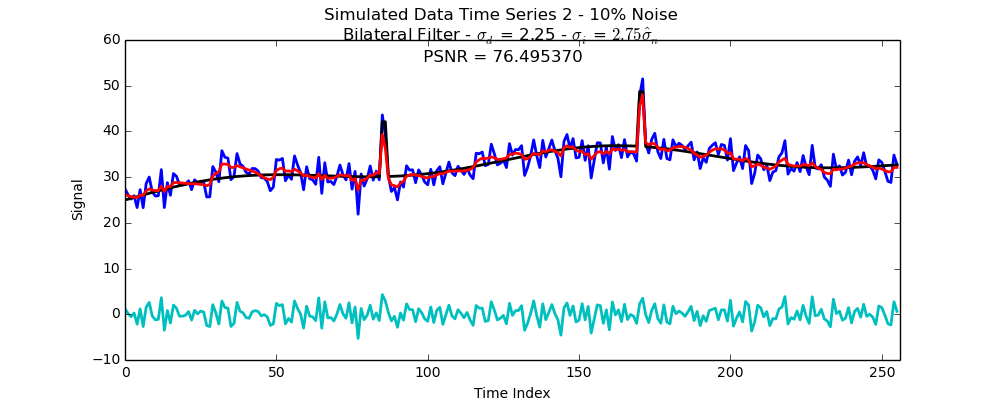
\includegraphics[width = 0.75 \textwidth]{BilateralSignal2Best.png}
\caption{Bilateral Filter - Best Denosing with 10\% Noise - Time Series 2}
\label{bilateral2best}
\end{figure}

\begin{figure}
\centering
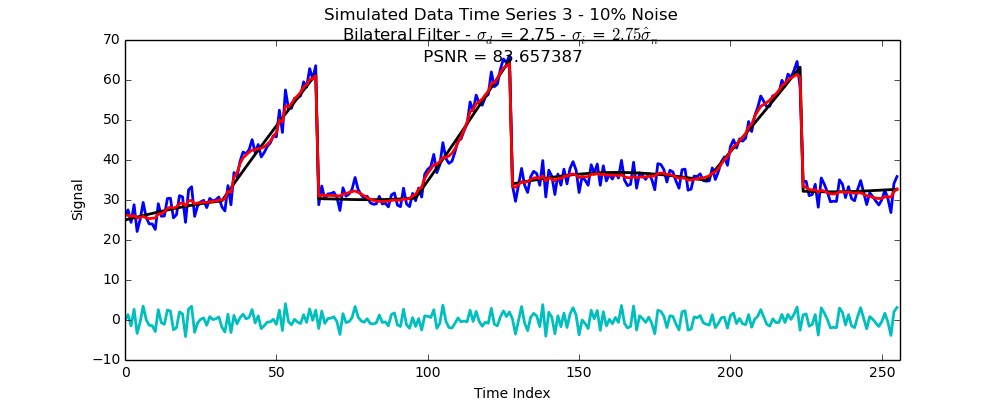
\includegraphics[width = 0.75 \textwidth]{BilateralSignal3Best.png}
\caption{Bilateral Filter - Best Denosing with 10\% Noise - Time Series 3}
\label{bilateral3best}
\end{figure}

\newpage

\subsubsection{Fast Fourier Transform Coefficient Thresholding}

The regression models are shown below, in Listings \ref{fftfilterseries1}, \ref{fftfilterseries2}, and \ref{fftfilterseries3}. There does not appear to be a single range of values that adequately captures the optimal performance of the hard threshold for Fast Fourier Transform Coefficient Thresholding. There are some methods for determining this automatically, such as SUREshrink.\\

Figures \ref{fft1best}, \ref{fft2best}, and \ref{fft3best} show the best performance of Fourier Transform Coefficient Thresholding for each time series.

{\footnotesize
\begin{lstlisting}[caption = Time Series 1 - FFT Coefficient Thresholding OLS Model, label = {fftfilterseries1}]
                            OLS Regression Results                            
==============================================================================
Dep. Variable:                   PSNR   R-squared:                       0.639
Model:                            OLS   Adj. R-squared:                  0.636
Method:                 Least Squares   F-statistic:                     192.5
Date:                Thu, 03 Jul 2014   Prob (F-statistic):           8.14e-72
Time:                        11:10:29   Log-Likelihood:                -959.58
No. Observations:                 330   AIC:                             1927.
Df Residuals:                     326   BIC:                             1942.
Df Model:                           3                                         
==================================================================================
                     coef    std err          t      P>|t|      [95.0% Conf. Int.]
----------------------------------------------------------------------------------
Intercept         64.1030      0.535    119.921      0.000        63.051    65.155
Noise             -0.4499      0.034    -13.142      0.000        -0.517    -0.383
Noise:Thresh       0.3822      0.038     10.099      0.000         0.308     0.457
I(Thresh ** 2)    -4.9605      0.273    -18.164      0.000        -5.498    -4.423
==============================================================================
Omnibus:                       16.985   Durbin-Watson:                   0.451
Prob(Omnibus):                  0.000   Jarque-Bera (JB):               10.551
Skew:                           0.292   Prob(JB):                      0.00511
Kurtosis:                       2.346   Cond. No.                         56.5
==============================================================================
\end{lstlisting}

\begin{lstlisting}[caption = Time Series 2 - FFT Coefficient Thresholding OLS Model, label = {fftfilterseries2}]
                           OLS Regression Results                            
==============================================================================
Dep. Variable:                   PSNR   R-squared:                       0.367
Model:                            OLS   Adj. R-squared:                  0.359
Method:                 Least Squares   F-statistic:                     47.03
Date:                Thu, 03 Jul 2014   Prob (F-statistic):           3.56e-31
Time:                        11:13:00   Log-Likelihood:                -997.94
No. Observations:                 330   AIC:                             2006.
Df Residuals:                     325   BIC:                             2025.
Df Model:                           4                                         
==================================================================================
                     coef    std err          t      P>|t|      [95.0% Conf. Int.]
----------------------------------------------------------------------------------
Intercept         64.2166      1.179     54.483      0.000        61.898    66.535
Noise             -0.5435      0.048    -11.215      0.000        -0.639    -0.448
Thresh            -8.7731      1.628     -5.387      0.000       -11.977    -5.569
Noise:Thresh       0.4428      0.051      8.695      0.000         0.343     0.543
I(Thresh ** 2)    -1.1040      0.458     -2.409      0.017        -2.006    -0.202
==============================================================================
Omnibus:                       85.081   Durbin-Watson:                   0.598
Prob(Omnibus):                  0.000   Jarque-Bera (JB):               22.878
Skew:                          -0.378   Prob(JB):                     1.08e-05
Kurtosis:                       1.955   Cond. No.                         180.
==============================================================================
\end{lstlisting}

\begin{lstlisting}[caption = Time Series 3 - FFT Coefficient Thresholding OLS Model, label = {fftfilterseries3}]
                            OLS Regression Results                            
==============================================================================
Dep. Variable:                   PSNR   R-squared:                       0.960
Model:                            OLS   Adj. R-squared:                  0.959
Method:                 Least Squares   F-statistic:                     1475.
Date:                Thu, 03 Jul 2014   Prob (F-statistic):          4.64e-170
Time:                        11:15:04   Log-Likelihood:                -609.28
No. Observations:                 250   AIC:                             1229.
Df Residuals:                     245   BIC:                             1246.
Df Model:                           4                                         
==================================================================================
                     coef    std err          t      P>|t|      [95.0% Conf. Int.]
----------------------------------------------------------------------------------
Intercept         70.5026      0.593    118.847      0.000        69.334    71.671
Noise             -0.3814      0.029    -12.942      0.000        -0.439    -0.323
Thresh           -33.2630      0.847    -39.261      0.000       -34.932   -31.594
Noise:Thresh       0.1622      0.016     10.112      0.000         0.131     0.194
I(Thresh ** 2)     6.2258      0.263     23.635      0.000         5.707     6.745
==============================================================================
Omnibus:                       28.319   Durbin-Watson:                   0.472
Prob(Omnibus):                  0.000   Jarque-Bera (JB):              111.060
Skew:                          -0.312   Prob(JB):                     7.65e-25
Kurtosis:                       6.205   Cond. No.                         195.
==============================================================================
\end{lstlisting}
}

\begin{figure}
\centering
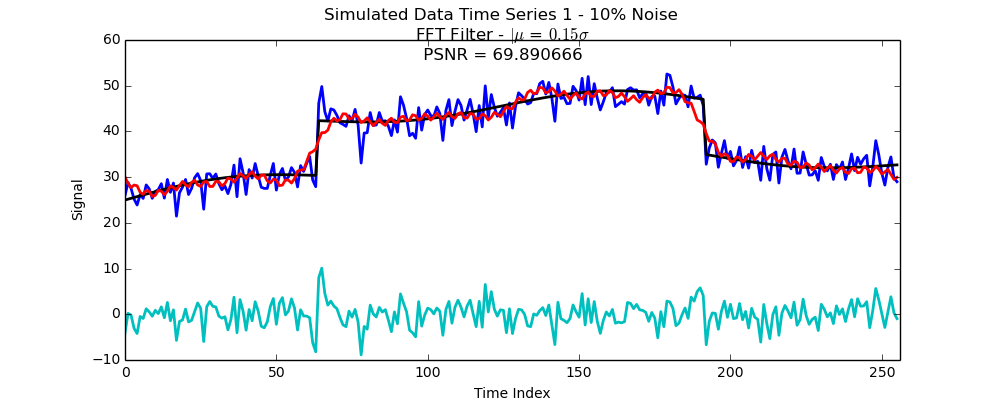
\includegraphics[width = 0.75 \textwidth]{FFTSignal1Best.png}
\caption{Fourier Transform Filter - Best Denosing with 10\% Noise - Time Series 1}
\label{fft1best}
\end{figure}

\begin{figure}
\centering
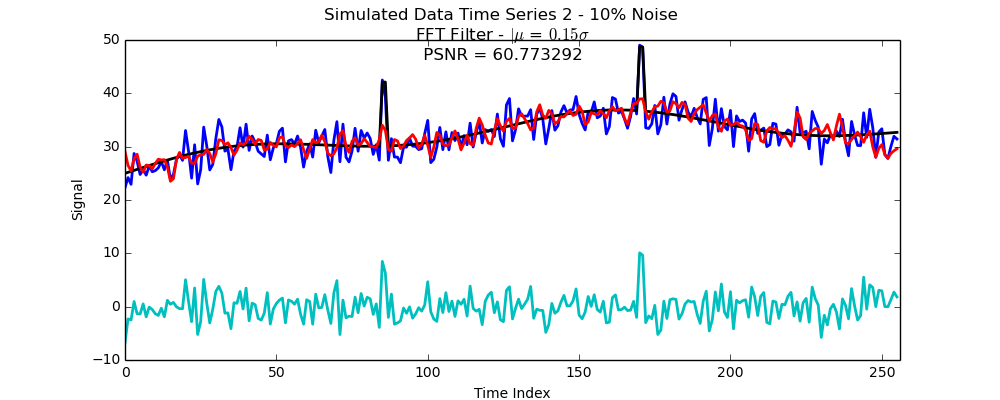
\includegraphics[width = 0.75 \textwidth]{FFTSignal2Best.png}
\caption{Fourier Transform Filter - Best Denosing with 10\% Noise - Time Series 2}
\label{fft2best}
\end{figure}

\begin{figure}
\centering
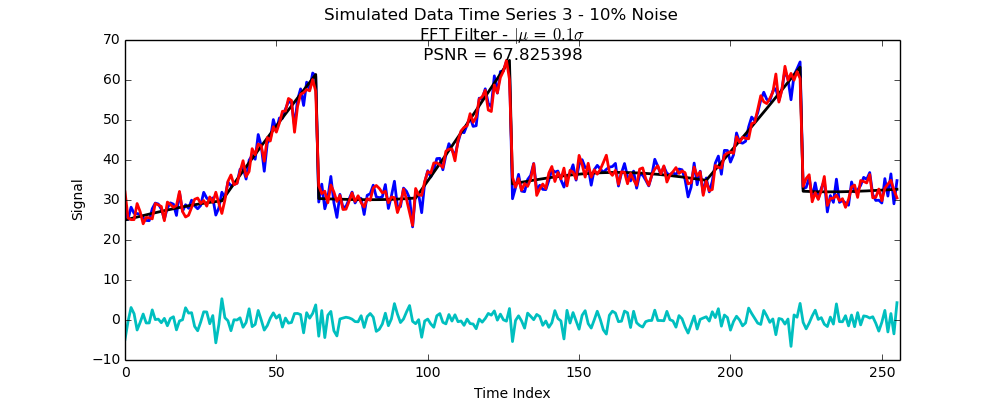
\includegraphics[width = 0.75 \textwidth]{FFTSignal3Best.png}
\caption{Fourier Transform Filter - Best Denosing with 10\% Noise - Time Series 3}
\label{fft3best}
\end{figure}

\newpage

\subsubsection{Wavelet Transform Coefficient Thresholding}

The regression models are shown below, in Listings \ref{waveletfilterseries1}, \ref{waveletfilterseries2}, and \ref{waveletfilterseries3}. Again, there does not appear to be a single range of values that adequately captures the optimal performance of the hard threshold for Wavelet Transform Coefficient Thresholding. There are some methods for determining this automatically, such as SUREshrink. Also note that there are a wide variety of wavelets, many of which give better performance than the Harr wavelet.\\

Figures \ref{wavelet1best}, \ref{wavelet2best}, and \ref{wavelet3best} show the best performance of Wavelet Transform Coefficient Thresholding for each time series.

{\footnotesize
\begin{lstlisting}[caption = Time Series 1 - Wavelet Coefficient Thresholding OLS Model, label = {waveletfilterseries1}]
                            OLS Regression Results                            
==============================================================================
Dep. Variable:                   PSNR   R-squared:                       0.942
Model:                            OLS   Adj. R-squared:                  0.941
Method:                 Least Squares   F-statistic:                     1082.
Date:                Thu, 03 Jul 2014   Prob (F-statistic):          8.89e-163
Time:                        11:27:07   Log-Likelihood:                -716.17
No. Observations:                 270   AIC:                             1442.
Df Residuals:                     265   BIC:                             1460.
Df Model:                           4                                         
==================================================================================
                     coef    std err          t      P>|t|      [95.0% Conf. Int.]
----------------------------------------------------------------------------------
Intercept         79.7083      0.803     99.249      0.000        78.127    81.290
Noise             -1.3502      0.032    -42.259      0.000        -1.413    -1.287
Thresh            -2.6478      1.443     -1.834      0.068        -5.490     0.194
Noise:Thresh       0.3449      0.037      9.292      0.000         0.272     0.418
I(Thresh ** 2)    -3.7036      0.400     -9.263      0.000        -4.491    -2.916
==============================================================================
Omnibus:                        0.530   Durbin-Watson:                   0.677
Prob(Omnibus):                  0.767   Jarque-Bera (JB):                0.616
Skew:                          -0.101   Prob(JB):                        0.735
Kurtosis:                       2.881   Cond. No.                         196.
==============================================================================
\end{lstlisting}

\begin{lstlisting}[caption = Time Series 2 - Wavelet Coefficient Thresholding OLS Model, label = {waveletfilterseries2}]
                            OLS Regression Results                            
==============================================================================
Dep. Variable:                   PSNR   R-squared:                       0.853
Model:                            OLS   Adj. R-squared:                  0.851
Method:                 Least Squares   F-statistic:                     405.7
Date:                Thu, 03 Jul 2014   Prob (F-statistic):          3.73e-115
Time:                        11:28:51   Log-Likelihood:                -650.64
No. Observations:                 285   AIC:                             1311.
Df Residuals:                     280   BIC:                             1330.
Df Model:                           4                                         
==================================================================================
                     coef    std err          t      P>|t|      [95.0% Conf. Int.]
----------------------------------------------------------------------------------
Intercept         72.5962      0.707    102.629      0.000        71.204    73.989
Noise             -1.0779      0.030    -36.272      0.000        -1.136    -1.019
Thresh           -16.5480      0.737    -22.452      0.000       -17.999   -15.097
Noise:Thresh       0.4817      0.023     21.025      0.000         0.437     0.527
I(Thresh ** 2)     2.2430      0.241      9.322      0.000         1.769     2.717
==============================================================================
Omnibus:                        0.702   Durbin-Watson:                   1.031
Prob(Omnibus):                  0.704   Jarque-Bera (JB):                0.719
Skew:                           0.119   Prob(JB):                        0.698
Kurtosis:                       2.938   Cond. No.                         179.
==============================================================================
\end{lstlisting}

\begin{lstlisting}[caption = Time Series 3 - Wavelet Coefficient Thresholding OLS Model, label = {waveletfilterseries3}]
                            OLS Regression Results                            
==============================================================================
Dep. Variable:                   PSNR   R-squared:                       0.884
Model:                            OLS   Adj. R-squared:                  0.883
Method:                 Least Squares   F-statistic:                     927.8
Date:                Thu, 03 Jul 2014   Prob (F-statistic):          1.21e-225
Time:                        11:31:00   Log-Likelihood:                -1492.0
No. Observations:                 490   AIC:                             2994.
Df Residuals:                     485   BIC:                             3015.
Df Model:                           4                                         
==================================================================================
                     coef    std err          t      P>|t|      [95.0% Conf. Int.]
----------------------------------------------------------------------------------
Intercept         88.7545      0.984     90.225      0.000        86.822    90.687
Noise             -1.0956      0.045    -24.499      0.000        -1.183    -1.008
Thresh           -18.8054      0.466    -40.358      0.000       -19.721   -17.890
Noise:Thresh       0.1878      0.011     17.454      0.000         0.167     0.209
I(Thresh ** 2)     1.3642      0.051     26.881      0.000         1.265     1.464
==============================================================================
Omnibus:                        9.341   Durbin-Watson:                   0.454
Prob(Omnibus):                  0.009   Jarque-Bera (JB):               15.700
Skew:                           0.001   Prob(JB):                     0.000390
Kurtosis:                       3.877   Cond. No.                         335.
==============================================================================
\end{lstlisting}
}

\begin{figure}
\centering
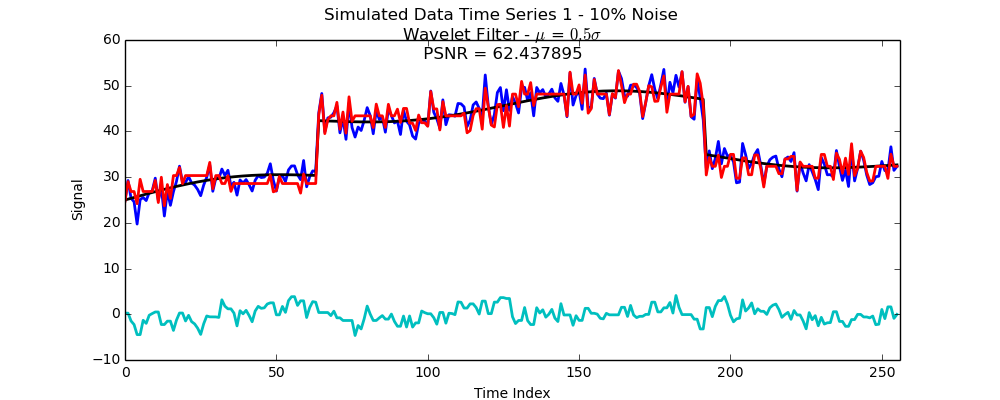
\includegraphics[width = 0.75 \textwidth]{WaveletSignal1Best.png}
\caption{Wavelet Transform Filter - Best Denosing with 10\% Noise - Time Series 1}
\label{wavelet1best}
\end{figure}

\begin{figure}
\centering
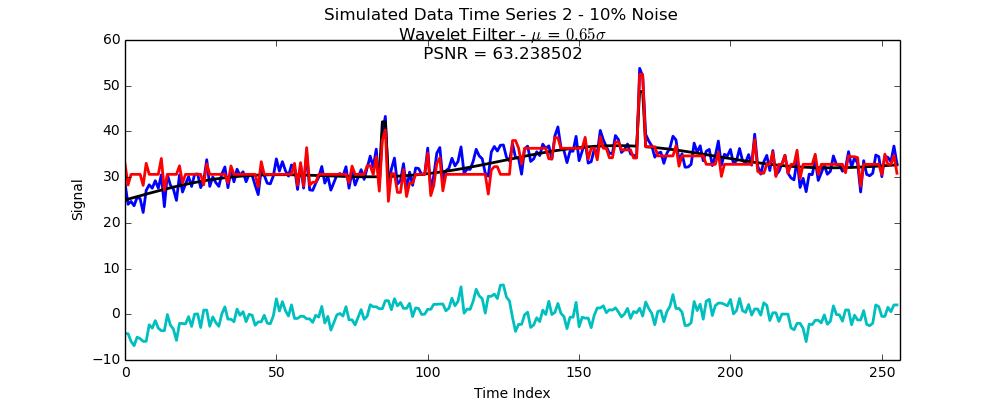
\includegraphics[width = 0.75 \textwidth]{WaveletSignal2Best.png}
\caption{Wavelet Transform Filter - Best Denosing with 10\% Noise - Time Series 2}
\label{wavelet2best}
\end{figure}

\begin{figure}
\centering
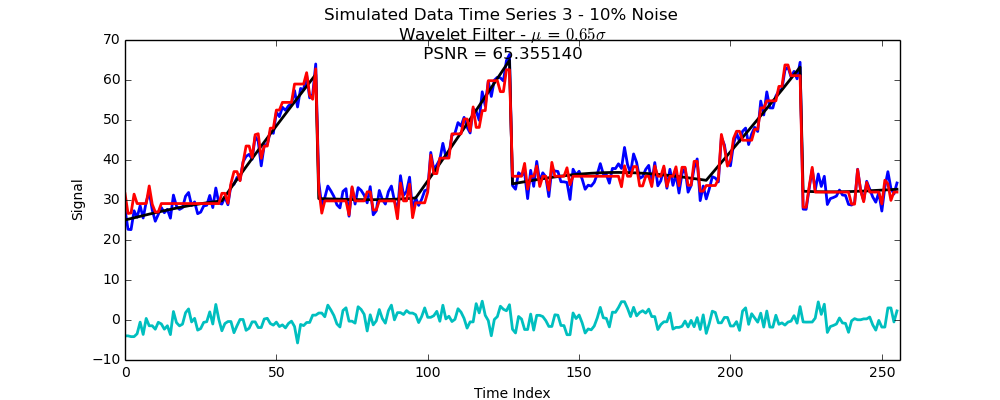
\includegraphics[width = 0.75 \textwidth]{WaveletSignal3Best.png}
\caption{Wavelet Transform Filter - Best Denosing with 10\% Noise - Time Series 3}
\label{wavelet3best}
\end{figure}

\newpage

\subsubsection{Non-Local Means}

The regression models are shown below, in Listings \ref{nlmeansfilterseries1}, \ref{nlmeansfilterseries2}, and \ref{nlmeansfilterseries3}. The best fit regression models do not clearly indicate optimal values of $\beta$, $\lvert I \rvert$, and $T$; however, running regression models for just $\beta$ and $T$ for each time series indicates that values of $T$ near $ 0.5 \left( max Y_j - min Y_j \right) \lvert I \rvert$ appear to be optimal (Listings \ref{nlmeanst1} and \ref{nlmeanst2}) while time series 3 indicates that $T$ has a minimum at close to that value (Listing \ref{nlmeanst3}). Time series 1 indicates $\beta$ close to $0.1$ is optimal (Listings \ref{nlmeansbeta1}) while time series 2 indicates that a value of $\beta$ closer to $0.8$ provides a minimum (Listing \ref{nlmeansbeta2}) and time series 3 provides an optimal value that is negative (Listing \ref{nlmeansbeta3}). The results for $\lvert I \rvert$ are even more sporadic. These results are inconsistent and confusing, to say the least.\\

Figures \ref{nlmeans1best}, \ref{nlmeans2best}, and \ref{nlmeans3best} show the best performance of the Non-Local Means filter for each time series.

{\footnotesize
\begin{lstlisting}[caption = Time Series 1 - Non-Local Means OLS Model, label = {nlmeansfilterseries1}]
                            OLS Regression Results                            
==============================================================================
Dep. Variable:                   PSNR   R-squared:                       0.836
Model:                            OLS   Adj. R-squared:                  0.836
Method:                 Least Squares   F-statistic:                     5425.
Date:                Thu, 03 Jul 2014   Prob (F-statistic):               0.00
Time:                        11:35:10   Log-Likelihood:                -18402.
No. Observations:                5320   AIC:                         3.682e+04
Df Residuals:                    5314   BIC:                         3.685e+04
Df Model:                           5                                         
==============================================================================
                 coef    std err          t      P>|t|      [95.0% Conf. Int.]
------------------------------------------------------------------------------
Intercept     91.7197      1.221     75.144      0.000        89.327    94.113
Noise         -1.5383      0.011   -137.209      0.000        -1.560    -1.516
Window         0.6392      0.047     13.548      0.000         0.547     0.732
Beta          -2.5589      1.505     -1.700      0.089        -5.509     0.392
T             24.2917      2.513      9.665      0.000        19.364    29.219
Beta:T       -24.9162      3.201     -7.783      0.000       -31.192   -18.641
==============================================================================
Omnibus:                      392.867   Durbin-Watson:                   0.147
Prob(Omnibus):                  0.000   Jarque-Bera (JB):              409.731
Skew:                           0.637   Prob(JB):                     1.07e-89
Kurtosis:                       2.525   Cond. No.                         802.
==============================================================================
\end{lstlisting}

\begin{lstlisting}[caption = Time Series 2 - Non-Local Means OLS Model, label = {nlmeansfilterseries2}]
                            OLS Regression Results                            
==============================================================================
Dep. Variable:                   PSNR   R-squared:                       0.831
Model:                            OLS   Adj. R-squared:                  0.831
Method:                 Least Squares   F-statistic:                     3813.
Date:                Thu, 03 Jul 2014   Prob (F-statistic):               0.00
Time:                        11:41:35   Log-Likelihood:                -13694.
No. Observations:                3880   AIC:                         2.740e+04
Df Residuals:                    3874   BIC:                         2.744e+04
Df Model:                           5                                         
==============================================================================
                 coef    std err          t      P>|t|      [95.0% Conf. Int.]
------------------------------------------------------------------------------
Intercept    115.8271      1.696     68.285      0.000       112.502   119.153
Noise         -1.6371      0.013   -122.142      0.000        -1.663    -1.611
Window         0.0688      0.059      1.160      0.246        -0.047     0.185
Beta         -22.6078      2.194    -10.305      0.000       -26.909   -18.307
T            -20.3645      2.661     -7.654      0.000       -25.581   -15.148
Beta:T        17.3624      3.438      5.050      0.000        10.621    24.103
==============================================================================
Omnibus:                     2871.829   Durbin-Watson:                   0.144
Prob(Omnibus):                  0.000   Jarque-Bera (JB):              282.493
Skew:                           0.295   Prob(JB):                     4.54e-62
Kurtosis:                       1.817   Cond. No.                         696.
==============================================================================
\end{lstlisting}

\begin{lstlisting}[caption = Time Series 3 - Non-Local Means OLS Model, label = {nlmeansfilterseries3}]
                            OLS Regression Results                            
==============================================================================
Dep. Variable:                   PSNR   R-squared:                       0.942
Model:                            OLS   Adj. R-squared:                  0.942
Method:                 Least Squares   F-statistic:                     2904.
Date:                Thu, 03 Jul 2014   Prob (F-statistic):               0.00
Time:                        11:45:33   Log-Likelihood:                -2402.1
No. Observations:                 900   AIC:                             4816.
Df Residuals:                     894   BIC:                             4845.
Df Model:                           5                                         
==============================================================================
                 coef    std err          t      P>|t|      [95.0% Conf. Int.]
------------------------------------------------------------------------------
Intercept     98.0358      1.226     79.974      0.000        95.630   100.442
Noise         -1.3228      0.011   -119.363      0.000        -1.345    -1.301
Window         0.4095      0.052      7.845      0.000         0.307     0.512
Beta          -9.3265      1.513     -6.164      0.000       -12.296    -6.357
T             -1.6236      2.178     -0.746      0.456        -5.898     2.650
Beta:T         1.9853      2.802      0.709      0.479        -3.513     7.484
==============================================================================
Omnibus:                        5.980   Durbin-Watson:                   0.516
Prob(Omnibus):                  0.050   Jarque-Bera (JB):                4.450
Skew:                          -0.026   Prob(JB):                        0.108
Kurtosis:                       2.659   Cond. No.                         596.
==============================================================================
\end{lstlisting}

\begin{lstlisting}[caption = Time Series 1 - Non-Local Means OLS Model - T Only, label = {nlmeanst1}]
                            OLS Regression Results                            
==============================================================================
Dep. Variable:                   PSNR   R-squared:                       0.094
Model:                            OLS   Adj. R-squared:                  0.094
Method:                 Least Squares   F-statistic:                     276.6
Date:                Thu, 03 Jul 2014   Prob (F-statistic):          5.07e-115
Time:                        11:33:49   Log-Likelihood:                -22950.
No. Observations:                5320   AIC:                         4.591e+04
Df Residuals:                    5317   BIC:                         4.593e+04
Df Model:                           2                                         
==============================================================================
                 coef    std err          t      P>|t|      [95.0% Conf. Int.]
------------------------------------------------------------------------------
Intercept     48.1040      1.096     43.882      0.000        45.955    50.253
T            123.5231      5.386     22.935      0.000       112.965   134.081
I(T ** 2)   -133.5808      6.477    -20.625      0.000      -146.278  -120.884
==============================================================================
Omnibus:                      415.917   Durbin-Watson:                   0.040
Prob(Omnibus):                  0.000   Jarque-Bera (JB):              485.561
Skew:                           0.718   Prob(JB):                    3.64e-106
Kurtosis:                       2.641   Cond. No.                         38.0
==============================================================================
\end{lstlisting}

\begin{lstlisting}[caption = Time Series 2 - Non-Local Means OLS Model - T Only, label = {nlmeanst2}]
                            OLS Regression Results                            
==============================================================================
Dep. Variable:                   PSNR   R-squared:                       0.158
Model:                            OLS   Adj. R-squared:                  0.158
Method:                 Least Squares   F-statistic:                     364.6
Date:                Thu, 03 Jul 2014   Prob (F-statistic):          8.11e-146
Time:                        11:40:28   Log-Likelihood:                -16810.
No. Observations:                3880   AIC:                         3.363e+04
Df Residuals:                    3877   BIC:                         3.364e+04
Df Model:                           2                                         
==============================================================================
                 coef    std err          t      P>|t|      [95.0% Conf. Int.]
------------------------------------------------------------------------------
Intercept     49.2915      2.630     18.739      0.000        44.134    54.449
T            112.5585      8.630     13.042      0.000        95.638   129.479
I(T ** 2)   -111.8098      6.605    -16.927      0.000      -124.760   -98.859
==============================================================================
Omnibus:                      682.418   Durbin-Watson:                   0.037
Prob(Omnibus):                  0.000   Jarque-Bera (JB):              214.717
Skew:                           0.340   Prob(JB):                     2.37e-47
Kurtosis:                       2.070   Cond. No.                         46.7
==============================================================================
\end{lstlisting}

\begin{lstlisting}[caption = Time Series 3 - Non-Local Means OLS Model - T Only, label = {nlmeanst3}]
                            OLS Regression Results                            
==============================================================================
Dep. Variable:                   PSNR   R-squared:                       0.000
Model:                            OLS   Adj. R-squared:                 -0.002
Method:                 Least Squares   F-statistic:                   0.01505
Date:                Thu, 03 Jul 2014   Prob (F-statistic):              0.985
Time:                        11:44:22   Log-Likelihood:                -3683.4
No. Observations:                 900   AIC:                             7373.
Df Residuals:                     897   BIC:                             7387.
Df Model:                           2                                         
==============================================================================
                 coef    std err          t      P>|t|      [95.0% Conf. Int.]
------------------------------------------------------------------------------
Intercept     76.5981      3.654     20.965      0.000        69.427    83.769
T             -2.8271     16.596     -0.170      0.865       -35.398    29.744
I(T ** 2)      2.6925     16.425      0.164      0.870       -29.544    34.929
==============================================================================
Omnibus:                     2095.720   Durbin-Watson:                   0.034
Prob(Omnibus):                  0.000   Jarque-Bera (JB):               64.272
Skew:                          -0.034   Prob(JB):                     1.11e-14
Kurtosis:                       1.693   Cond. No.                         56.7
==============================================================================
\end{lstlisting}

\begin{lstlisting}[caption = Time Series 1 - Non-Local Means OLS Model - $\beta$ Only, label = {nlmeansbeta1}]
                            OLS Regression Results                            
==============================================================================
Dep. Variable:                   PSNR   R-squared:                       0.212
Model:                            OLS   Adj. R-squared:                  0.211
Method:                 Least Squares   F-statistic:                     713.5
Date:                Thu, 03 Jul 2014   Prob (F-statistic):          3.21e-275
Time:                        11:32:40   Log-Likelihood:                -22581.
No. Observations:                5320   AIC:                         4.517e+04
Df Residuals:                    5317   BIC:                         4.519e+04
Df Model:                           2                                         
================================================================================
                   coef    std err          t      P>|t|      [95.0% Conf. Int.]
--------------------------------------------------------------------------------
Intercept       88.3550      4.785     18.464      0.000        78.974    97.736
Beta             6.3853     13.518      0.472      0.637       -20.116    32.887
I(Beta ** 2)   -34.9954      9.025     -3.878      0.000       -52.688   -17.302
==============================================================================
Omnibus:                      183.932   Durbin-Watson:                   0.038
Prob(Omnibus):                  0.000   Jarque-Bera (JB):              172.779
Skew:                           0.394   Prob(JB):                     3.03e-38
Kurtosis:                       2.601   Cond. No.                         101.
==============================================================================
\end{lstlisting}

\begin{lstlisting}[caption = Time Series 2 - Non-Local Means OLS Model - $\beta$ Only, label = {nlmeansbeta2}]
                            OLS Regression Results                            
==============================================================================
Dep. Variable:                   PSNR   R-squared:                       0.132
Model:                            OLS   Adj. R-squared:                  0.131
Method:                 Least Squares   F-statistic:                     294.1
Date:                Thu, 03 Jul 2014   Prob (F-statistic):          1.23e-119
Time:                        11:39:27   Log-Likelihood:                -16870.
No. Observations:                3880   AIC:                         3.375e+04
Df Residuals:                    3877   BIC:                         3.377e+04
Df Model:                           2                                         
================================================================================
                   coef    std err          t      P>|t|      [95.0% Conf. Int.]
--------------------------------------------------------------------------------
Intercept      186.2135      5.983     31.123      0.000       174.483   197.944
Beta          -294.9086     16.870    -17.481      0.000      -327.984  -261.833
I(Beta ** 2)   177.9004     11.250     15.813      0.000       155.844   199.957
==============================================================================
Omnibus:                      304.504   Durbin-Watson:                   0.032
Prob(Omnibus):                  0.000   Jarque-Bera (JB):              260.360
Skew:                           0.558   Prob(JB):                     2.91e-57
Kurtosis:                       2.394   Cond. No.                         96.5
==============================================================================
\end{lstlisting}

\begin{lstlisting}[caption = Time Series 3 - Non-Local Means OLS Model - $\beta$ Only, label = {nlmeansbeta3}]
                            OLS Regression Results                            
==============================================================================
Dep. Variable:                   PSNR   R-squared:                       0.014
Model:                            OLS   Adj. R-squared:                  0.012
Method:                 Least Squares   F-statistic:                     6.280
Date:                Thu, 03 Jul 2014   Prob (F-statistic):            0.00196
Time:                        11:43:21   Log-Likelihood:                -3677.2
No. Observations:                 900   AIC:                             7360.
Df Residuals:                     897   BIC:                             7375.
Df Model:                           2                                         
================================================================================
                   coef    std err          t      P>|t|      [95.0% Conf. Int.]
--------------------------------------------------------------------------------
Intercept       80.7228      8.691      9.288      0.000        63.666    97.779
Beta            -4.0212     24.581     -0.164      0.870       -52.264    44.222
I(Beta ** 2)    -2.8751     16.312     -0.176      0.860       -34.889    29.139
==============================================================================
Omnibus:                        0.677   Durbin-Watson:                   0.036
Prob(Omnibus):                  0.713   Jarque-Bera (JB):               72.795
Skew:                          -0.067   Prob(JB):                     1.56e-16
Kurtosis:                       1.613   Cond. No.                         90.1
==============================================================================
\end{lstlisting}
}

\begin{figure}
\centering
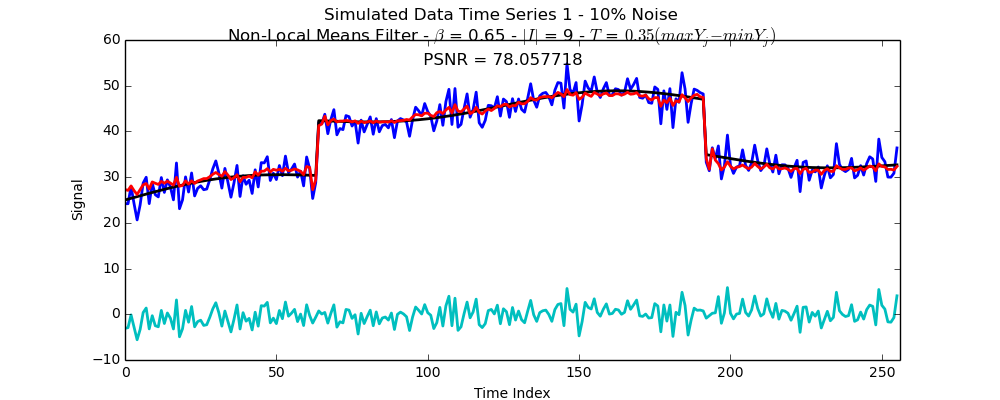
\includegraphics[width = 0.75 \textwidth]{NLMeansSignal1Best.png}
\caption{Non-Local Means Filter - Best Denosing with 10\% Noise - Time Series 1}
\label{nlmeans1best}
\end{figure}

\begin{figure}
\centering
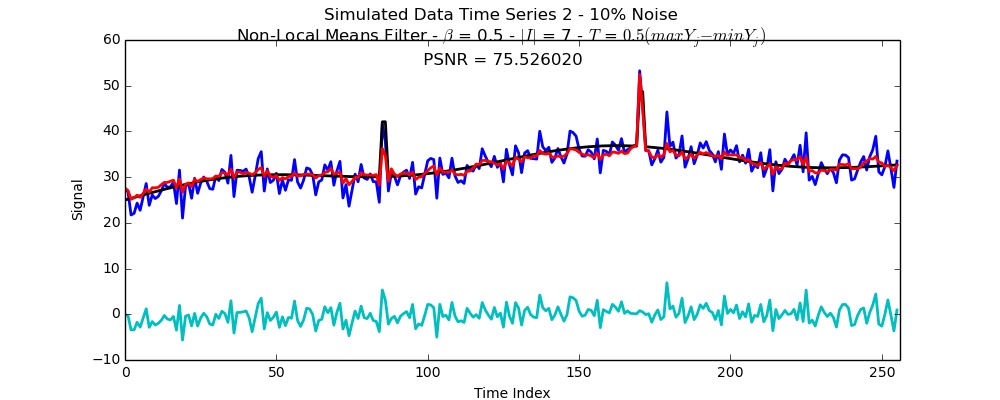
\includegraphics[width = 0.75 \textwidth]{NLMeansSignal2Best.png}
\caption{Non-Local Means Filter - Best Denosing with 10\% Noise - Time Series 2}
\label{nlmeans2best}
\end{figure}

\begin{figure}
\centering
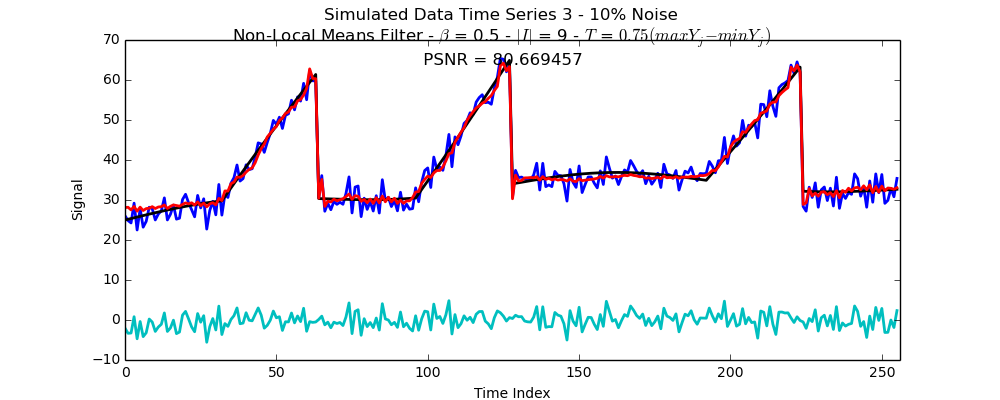
\includegraphics[width = 0.75 \textwidth]{NLMeansSignal3Best.png}
\caption{Non-Local Means Filter - Best Denosing with 10\% Noise - Time Series 3}
\label{nlmeans3best}
\end{figure}

\newpage


\subsubsection{Iterated Bilateral Filter}

When iterating the Bilateral filter, two different techniques come to mind. First, we could iterate using the same Bilateral filter, i.e. using the same $\sigma_d$ and $\sigma_i$, each time. Alternatively we could modify the parameters for each iteration. The second approach offers more flexibility but increases complexity as there are more parameters to select. We will investigate both.\\

For these investigations, I only considered the three time series with $10$\% added noise.\\

Keeping the same smoothing parameters, $\sigma_d$ and $\sigma_i$, for each iteration of the Bilateral filter means that this implementation of iterated Bilateral filter is simpler, as the analyst only has two parameters to choose. We will first consider two iterations of the same Bilateral filter and then consider iterating the same Bilateral filter until the difference between two iterations are within some tolerance.

\paragraph{Same Parameters - Two Iterations}

Unfortunately, the optimal performance of the two iterations of the Bilateral filter is not as predictable as the optimal performance of the Bilateral filter. Iterating at the optimal values for a single iteration can in fact lead to a lower PSNR value and degradation of the time series.

{\footnotesize
\begin{lstlisting}[caption = Time Series 1 - Bilateral Filter 2 Same Iterations OLS Model, label = {2samebilateral1}]
                            OLS Regression Results                            
==============================================================================
Dep. Variable:                   PSNR   R-squared:                       0.848
Model:                            OLS   Adj. R-squared:                  0.848
Method:                 Least Squares   F-statistic:                     5013.
Date:                Tue, 15 Jul 2014   Prob (F-statistic):               0.00
Time:                        15:11:54   Log-Likelihood:                -9628.0
No. Observations:                2700   AIC:                         1.926e+04
Df Residuals:                    2696   BIC:                         1.929e+04
Df Model:                           3                                         
==============================================================================
                 coef    std err          t      P>|t|      [95.0% Conf. Int.]
------------------------------------------------------------------------------
Intercept    105.5318      2.282     46.247      0.000       101.057   110.006
Noise         -1.9181      0.016   -122.572      0.000        -1.949    -1.887
SigD           1.6288      0.408      3.996      0.000         0.830     2.428
SigI           0.9404      0.691      1.360      0.174        -0.415     2.296
==============================================================================
Omnibus:                     1763.412   Durbin-Watson:                   0.178
Prob(Omnibus):                  0.000   Jarque-Bera (JB):              200.317
Skew:                           0.322   Prob(JB):                     3.17e-44
Kurtosis:                       1.831   Cond. No.                         247.
==============================================================================
\end{lstlisting}

\begin{lstlisting}[caption = Time Series 2 - Bilateral Filter 2 Same Iterations OLS Model, label = {2samebilateral2}]
                            OLS Regression Results                            
==============================================================================
Dep. Variable:                   PSNR   R-squared:                       0.835
Model:                            OLS   Adj. R-squared:                  0.835
Method:                 Least Squares   F-statistic:                     3030.
Date:                Tue, 15 Jul 2014   Prob (F-statistic):               0.00
Time:                        15:11:33   Log-Likelihood:                -6738.0
No. Observations:                1800   AIC:                         1.348e+04
Df Residuals:                    1796   BIC:                         1.351e+04
Df Model:                           3                                         
==============================================================================
                 coef    std err          t      P>|t|      [95.0% Conf. Int.]
------------------------------------------------------------------------------
Intercept    111.9833      3.504     31.961      0.000       105.112   118.855
Noise         -2.1823      0.023    -95.320      0.000        -2.227    -2.137
SigD           0.9691      0.815      1.189      0.235        -0.630     2.568
SigI          -0.6262      0.770     -0.813      0.416        -2.136     0.884
==============================================================================
Omnibus:                     2084.582   Durbin-Watson:                   0.189
Prob(Omnibus):                  0.000   Jarque-Bera (JB):              131.634
Skew:                           0.234   Prob(JB):                     2.61e-29
Kurtosis:                       1.761   Cond. No.                         258.
==============================================================================
\end{lstlisting}

\begin{lstlisting}[caption = Time Series 3 - Bilateral Filter 2 Same Iterations OLS Model, label = {2samebilateral3}]
                            OLS Regression Results                            
==============================================================================
Dep. Variable:                   PSNR   R-squared:                       0.955
Model:                            OLS   Adj. R-squared:                  0.955
Method:                 Least Squares   F-statistic:                 2.221e+04
Date:                Tue, 15 Jul 2014   Prob (F-statistic):               0.00
Time:                        15:11:08   Log-Likelihood:                -8154.9
No. Observations:                3150   AIC:                         1.632e+04
Df Residuals:                    3146   BIC:                         1.634e+04
Df Model:                           3                                         
==============================================================================
                 coef    std err          t      P>|t|      [95.0% Conf. Int.]
------------------------------------------------------------------------------
Intercept    108.8374      0.989    110.102      0.000       106.899   110.776
Noise         -1.4066      0.005   -257.954      0.000        -1.417    -1.396
SigD          -2.4011      0.252     -9.526      0.000        -2.895    -1.907
SigI          -0.5449      0.223     -2.446      0.014        -0.982    -0.108
==============================================================================
Omnibus:                       13.638   Durbin-Watson:                   0.854
Prob(Omnibus):                  0.001   Jarque-Bera (JB):               11.093
Skew:                          -0.065   Prob(JB):                      0.00390
Kurtosis:                       2.740   Cond. No.                         306.
==============================================================================
\end{lstlisting}
}

\begin{figure}
\centering
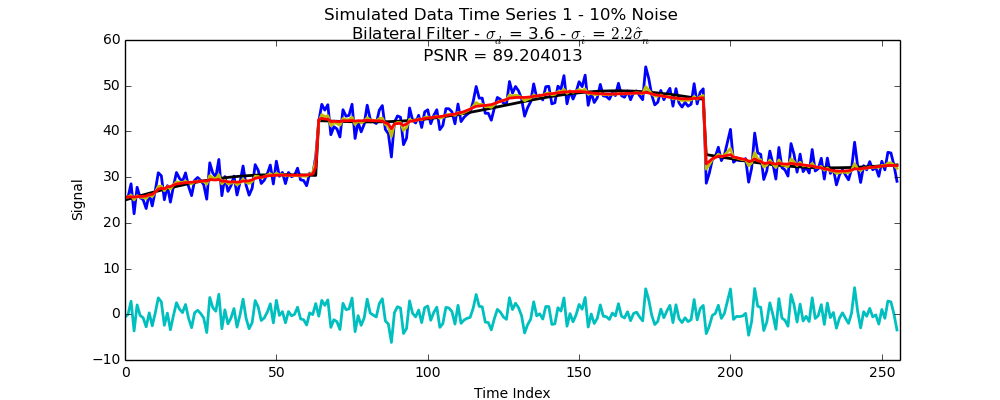
\includegraphics[width = 0.75 \textwidth]{2SameBilateralSignal1Best.png}
\caption{Bilateral Filter - 2 Same Iterations - Best Denosing with 10\% Noise - Time Series 1}
\label{2samebilateral1best}
\end{figure}

\begin{figure}
\centering
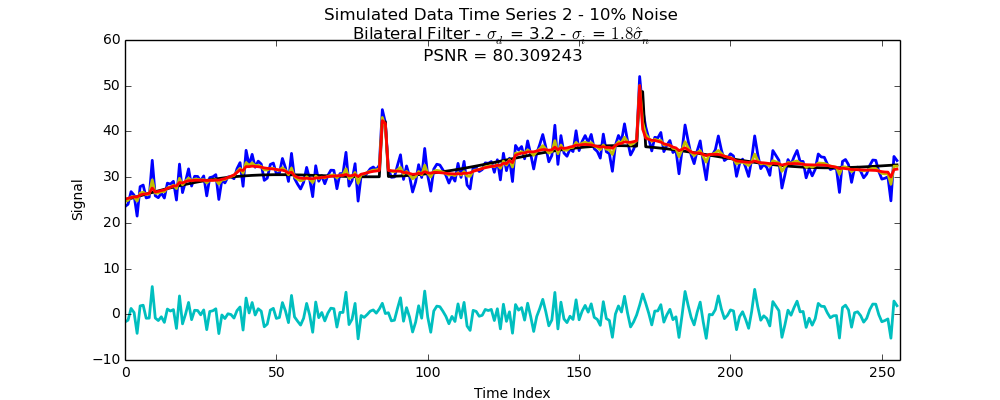
\includegraphics[width = 0.75 \textwidth]{2SameBilateralSignal2Best.png}
\caption{Bilateral Filter - 2 Same Iterations - Best Denosing with 10\% Noise - Time Series 2}
\label{2samebilateral2best}
\end{figure}

\begin{figure}
\centering
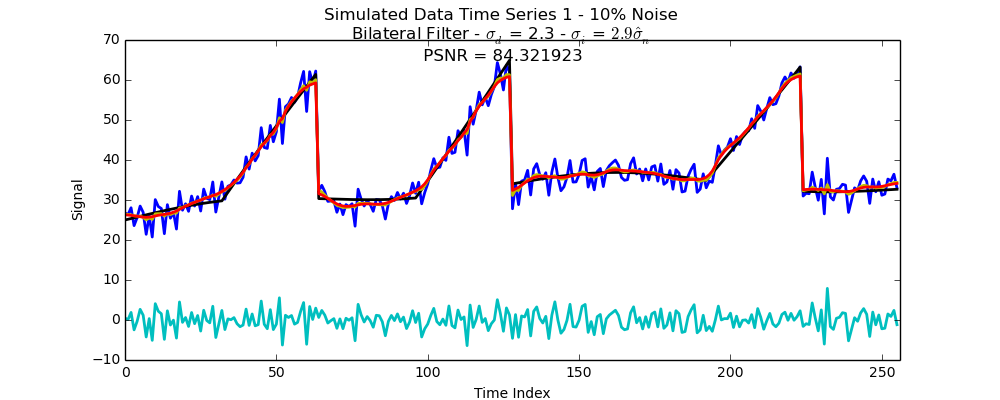
\includegraphics[width = 0.75 \textwidth]{2SameBilateralSignal3Best.png}
\caption{Bilateral Filter - 2 Same Iterations - Best Denosing with 10\% Noise - Time Series 3}
\label{2samebilateral3best}
\end{figure}

\newpage

\paragraph{Same Parameters - Iterated to Tolerance}

In this case, the Bilateral filter was iterated until there was less than $1$\% difference between the iterations. The optimal performance of multiple iterations of the Bilateral filter is also not as predictable as the optimal performance of the Bilateral filter. Iterating at the optimal values for a single iteration can again in fact lead to a lower PSNR value and degradation of the time series.

{\footnotesize
\begin{lstlisting}[caption = Time Series 1 - Bilateral Filter Multiple Iterations OLS Model, label = {itrsamebilateral1}]
                            OLS Regression Results                            
==============================================================================
Dep. Variable:                   PSNR   R-squared:                       0.846
Model:                            OLS   Adj. R-squared:                  0.846
Method:                 Least Squares   F-statistic:                     4110.
Date:                Tue, 15 Jul 2014   Prob (F-statistic):               0.00
Time:                        14:07:07   Log-Likelihood:                -8051.9
No. Observations:                2250   AIC:                         1.611e+04
Df Residuals:                    2246   BIC:                         1.613e+04
Df Model:                           3                                         
==============================================================================
                 coef    std err          t      P>|t|      [95.0% Conf. Int.]
------------------------------------------------------------------------------
Intercept    105.7915      3.563     29.692      0.000        98.804   112.778
Noise         -1.9277      0.017   -111.013      0.000        -1.962    -1.894
SigD           1.6114      0.686      2.348      0.019         0.266     2.957
SigI           1.0059      1.129      0.891      0.373        -1.208     3.219
==============================================================================
Omnibus:                     2004.463   Durbin-Watson:                   0.191
Prob(Omnibus):                  0.000   Jarque-Bera (JB):              164.947
Skew:                           0.273   Prob(JB):                     1.52e-36
Kurtosis:                       1.791   Cond. No.                         348.
==============================================================================
\end{lstlisting}

\begin{lstlisting}[caption = Time Series 2 - Bilateral Filter Multiple Iterations OLS Model, label = {itrsamebilateral2}]
                            OLS Regression Results                            
==============================================================================
Dep. Variable:                   PSNR   R-squared:                       0.843
Model:                            OLS   Adj. R-squared:                  0.843
Method:                 Least Squares   F-statistic:                     3221.
Date:                Tue, 15 Jul 2014   Prob (F-statistic):               0.00
Time:                        14:07:25   Log-Likelihood:                -6640.6
No. Observations:                1800   AIC:                         1.329e+04
Df Residuals:                    1796   BIC:                         1.331e+04
Df Model:                           3                                         
==============================================================================
                 coef    std err          t      P>|t|      [95.0% Conf. Int.]
------------------------------------------------------------------------------
Intercept    114.0006      3.419     33.343      0.000       107.295   120.706
Noise         -2.1318      0.022    -98.293      0.000        -2.174    -2.089
SigD           0.0582      0.513      0.113      0.910        -0.949     1.065
SigI          -0.6043      0.896     -0.674      0.500        -2.362     1.154
==============================================================================
Omnibus:                      680.671   Durbin-Watson:                   0.217
Prob(Omnibus):                  0.000   Jarque-Bera (JB):               97.644
Skew:                           0.163   Prob(JB):                     6.26e-22
Kurtosis:                       1.906   Cond. No.                         268.
==============================================================================
\end{lstlisting}

\begin{lstlisting}[caption = Time Series 3 - Bilateral Filter Multiple Iterations OLS Model, label = {itrsamebilateral3}]
                            OLS Regression Results                            
==============================================================================
Dep. Variable:                   PSNR   R-squared:                       0.901
Model:                            OLS   Adj. R-squared:                  0.901
Method:                 Least Squares   F-statistic:                     5454.
Date:                Tue, 15 Jul 2014   Prob (F-statistic):               0.00
Time:                        14:07:50   Log-Likelihood:                -5519.7
No. Observations:                1800   AIC:                         1.105e+04
Df Residuals:                    1796   BIC:                         1.107e+04
Df Model:                           3                                         
==============================================================================
                 coef    std err          t      P>|t|      [95.0% Conf. Int.]
------------------------------------------------------------------------------
Intercept    106.3716      0.876    121.377      0.000       104.653   108.090
Noise         -1.4870      0.012   -127.798      0.000        -1.510    -1.464
SigD          -0.6899      0.303     -2.277      0.023        -1.284    -0.096
SigI          -0.8320      0.449     -1.853      0.064        -1.713     0.049
==============================================================================
Omnibus:                      314.669   Durbin-Watson:                   0.320
Prob(Omnibus):                  0.000   Jarque-Bera (JB):              601.856
Skew:                           1.056   Prob(JB):                    2.04e-131
Kurtosis:                       4.889   Cond. No.                         135.
==============================================================================
\end{lstlisting}
}

\begin{figure}
\centering
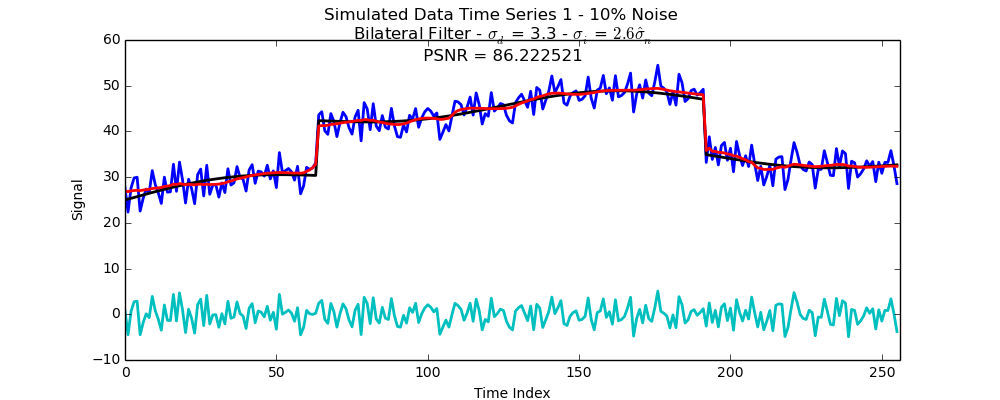
\includegraphics[width = 0.75 \textwidth]{ItrSameBilateralSignal1Best.png}
\caption{Bilateral Filter - Multiple Iterations - Best Denosing with 10\% Noise - Time Series 1}
\label{itrsamebilateral1best}
\end{figure}

\begin{figure}
\centering
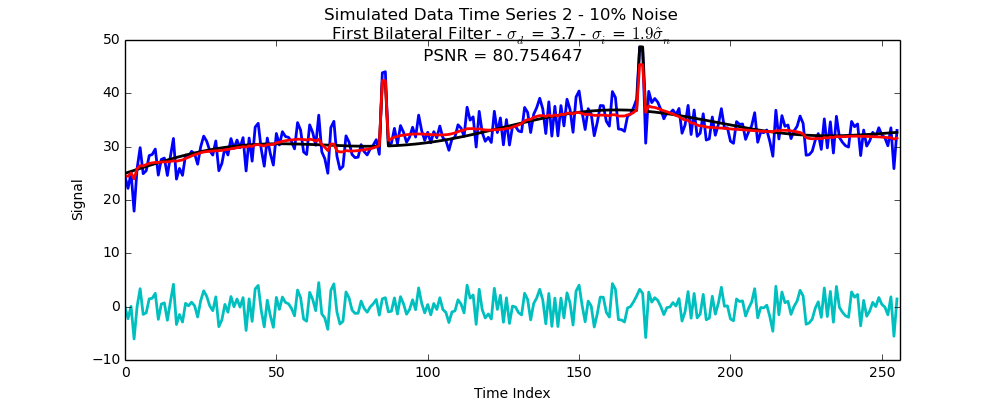
\includegraphics[width = 0.75 \textwidth]{ItrSameBilateralSignal2Best.png}
\caption{Bilateral Filter - Multiple Iterations - Best Denosing with 10\% Noise - Time Series 2}
\label{itrsamebilateral2best}
\end{figure}

\begin{figure}
\centering
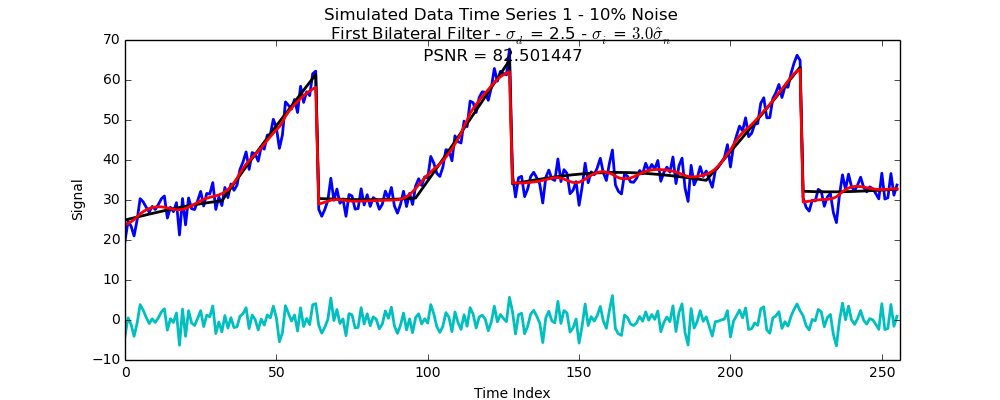
\includegraphics[width = 0.75 \textwidth]{ItrSameBilateralSignal3Best.png}
\caption{Bilateral Filter - Multiple Iterations - Best Denosing with 10\% Noise - Time Series 3}
\label{itrsamebilateral3best}
\end{figure}

\newpage

\paragraph{Different Parameters - Two Iterations}

When we allow for different parameters, $\sigma_d$ and $\sigma_i$, between iterations of the bilateral filter, the filter becomes much more complex. There are two additional parameters for each iteration of the Bilateral filter. To keep from running away with complexity, we will investigate using the Bilateral filter twice, with different parameters between each iteration.\\

When we add the second filter, the optimal performance of the Bilateral filter is not as predictable as the optimal performance of the Bilateral filter. Iterating at the optimal values for a single iteration can in fact lead to a lower PSNR value and degradation of the time series.

{\footnotesize
\begin{lstlisting}[caption = Time Series 1 - Bilateral Filter 2 Different Iterations OLS Model, label = {2diffbilateral1}]
                            OLS Regression Results                            
==============================================================================
Dep. Variable:                   PSNR   R-squared:                       0.843
Model:                            OLS   Adj. R-squared:                  0.843
Method:                 Least Squares   F-statistic:                 1.351e+04
Date:                Tue, 15 Jul 2014   Prob (F-statistic):               0.00
Time:                        17:11:49   Log-Likelihood:                -45241.
No. Observations:               12550   AIC:                         9.049e+04
Df Residuals:                   12544   BIC:                         9.054e+04
Df Model:                           5                                         
==============================================================================
                 coef    std err          t      P>|t|      [95.0% Conf. Int.]
------------------------------------------------------------------------------
Intercept    105.9011      1.731     61.192      0.000       102.509   109.293
Noise         -1.9603      0.008   -259.902      0.000        -1.975    -1.946
SigD1          1.0138      0.282      3.594      0.000         0.461     1.567
SigI1          0.4591      0.350      1.312      0.189        -0.227     1.145
SigD2          0.5848      0.344      1.698      0.090        -0.090     1.260
SigI2          0.6720      0.302      2.223      0.026         0.079     1.265
==============================================================================
Omnibus:                    17230.689   Durbin-Watson:                   0.147
Prob(Omnibus):                  0.000   Jarque-Bera (JB):             1010.214
Skew:                           0.312   Prob(JB):                    4.31e-220
Kurtosis:                       1.758   Cond. No.                         386.
==============================================================================
\end{lstlisting}

\begin{lstlisting}[caption = Time Series 2 - Bilateral Filter 2 Different Iterations OLS Model, label = {2diffbilateral2}]
                            OLS Regression Results                            
==============================================================================
Dep. Variable:                   PSNR   R-squared:                       0.835
Model:                            OLS   Adj. R-squared:                  0.835
Method:                 Least Squares   F-statistic:                     8596.
Date:                Tue, 15 Jul 2014   Prob (F-statistic):               0.00
Time:                        17:12:12   Log-Likelihood:                -31912.
No. Observations:                8500   AIC:                         6.384e+04
Df Residuals:                    8494   BIC:                         6.388e+04
Df Model:                           5                                         
==============================================================================
                 coef    std err          t      P>|t|      [95.0% Conf. Int.]
------------------------------------------------------------------------------
Intercept    113.5447      2.483     45.737      0.000       108.678   118.411
Noise         -2.2059      0.011   -207.250      0.000        -2.227    -2.185
SigD1          0.0868      0.467      0.186      0.852        -0.829     1.002
SigI1         -1.0205      0.399     -2.556      0.011        -1.803    -0.238
SigD2          0.6662      0.399      1.668      0.095        -0.116     1.449
SigI2          0.0509      0.464      0.110      0.913        -0.859     0.961
==============================================================================
Omnibus:                    16181.260   Durbin-Watson:                   0.154
Prob(Omnibus):                  0.000   Jarque-Bera (JB):              668.067
Skew:                           0.264   Prob(JB):                    8.53e-146
Kurtosis:                       1.732   Cond. No.                         392.
==============================================================================
\end{lstlisting}

\begin{lstlisting}[caption = Time Series 3 - Bilateral Filter 2 Different Iterations OLS Model, label = {2diffbilateral3}]
                            OLS Regression Results                            
==============================================================================
Dep. Variable:                   PSNR   R-squared:                       0.959
Model:                            OLS   Adj. R-squared:                  0.959
Method:                 Least Squares   F-statistic:                 3.953e+04
Date:                Tue, 15 Jul 2014   Prob (F-statistic):               0.00
Time:                        17:12:32   Log-Likelihood:                -21502.
No. Observations:                8500   AIC:                         4.302e+04
Df Residuals:                    8494   BIC:                         4.306e+04
Df Model:                           5                                         
==============================================================================
                 coef    std err          t      P>|t|      [95.0% Conf. Int.]
------------------------------------------------------------------------------
Intercept    108.5808      0.732    148.311      0.000       107.146   110.016
Noise         -1.3900      0.003   -444.369      0.000        -1.396    -1.384
SigD1         -1.3004      0.121    -10.745      0.000        -1.538    -1.063
SigI1         -0.7309      0.117     -6.262      0.000        -0.960    -0.502
SigD2         -1.0483      0.146     -7.193      0.000        -1.334    -0.763
SigI2          0.1334      0.144      0.930      0.352        -0.148     0.415
==============================================================================
Omnibus:                       52.024   Durbin-Watson:                   0.940
Prob(Omnibus):                  0.000   Jarque-Bera (JB):               51.141
Skew:                          -0.172   Prob(JB):                     7.85e-12
Kurtosis:                       2.840   Cond. No.                         394.
==============================================================================
\end{lstlisting}
}

\begin{figure}
\centering
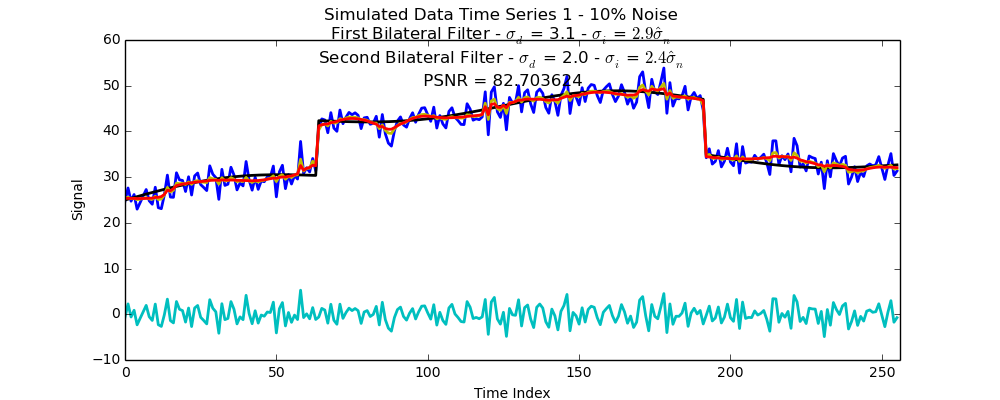
\includegraphics[width = 0.75 \textwidth]{2DiffBilateralSignal1Best.png}
\caption{Bilateral Filter - 2 Different Iterations - Best Denosing with 10\% Noise - Time Series 1}
\label{2diffbilateral1best}
\end{figure}

\begin{figure}
\centering
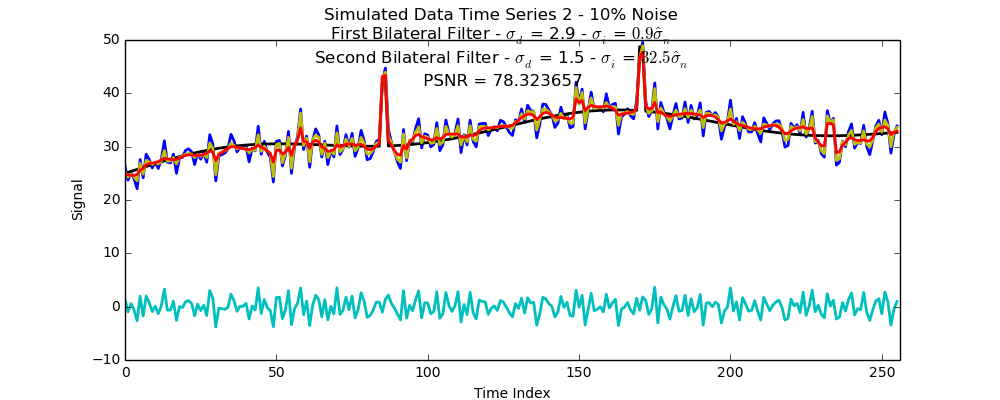
\includegraphics[width = 0.75 \textwidth]{2DiffBilateralSignal2Best.png}
\caption{Bilateral Filter - 2 Different Iterations - Best Denosing with 10\% Noise - Time Series 2}
\label{2diffbilateral2best}
\end{figure}

\begin{figure}
\centering
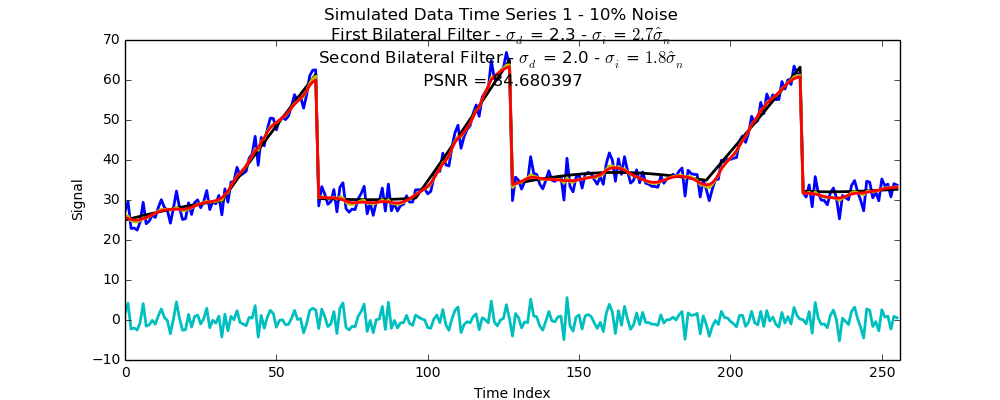
\includegraphics[width = 0.75 \textwidth]{2DiffBilateralSignal3Best.png}
\caption{Bilateral Filter - 2 Different Iterations - Best Denosing with 10\% Noise - Time Series 3}
\label{2diffbilateral3best}
\end{figure}

\newpage

\paragraph{Conclusions}

It appears that while iterating the Bilateral filter can increase performance of the denosing, it makes it difficult to chose the optimal parameters. One of the strongest benefits of the Bilateral filter is the apparent robustness of the optimal range of parameters, and this advantage is lost when iterating the Bilateral filter.

\subsubsection{Iterated Non-Local Means Filter}

The Non-Local Means filter is much more complex than the Bilateral filter. Due to this fact, we will only investigate iterating the Non-Local Means filter with the same parameters on each iteration. We will consider two iterations of Non-Local Means filter.\\

Optimal parameters for two iterations of the Non-Local Means are as unpredictable as for Non-Local Means.

{\footnotesize
\begin{lstlisting}[caption = Time Series 1 - Non-Local Means Filter 2 Iterations OLS Model, label = {multinlmeans1}]
                            OLS Regression Results                            
==============================================================================
Dep. Variable:                   PSNR   R-squared:                       0.870
Model:                            OLS   Adj. R-squared:                  0.870
Method:                 Least Squares   F-statistic:                     2140.
Date:                Wed, 16 Jul 2014   Prob (F-statistic):               0.00
Time:                        12:42:18   Log-Likelihood:                -5113.9
No. Observations:                1600   AIC:                         1.024e+04
Df Residuals:                    1594   BIC:                         1.027e+04
Df Model:                           5                                         
==============================================================================
                 coef    std err          t      P>|t|      [95.0% Conf. Int.]
------------------------------------------------------------------------------
Intercept    100.5099      1.176     85.448      0.000        98.203   102.817
Noise         -1.4535      0.014   -103.364      0.000        -1.481    -1.426
Beta1         -4.6183      1.253     -3.686      0.000        -7.076    -2.161
T1             0.4735      1.092      0.434      0.665        -1.668     2.615
Beta2         -2.3095      1.150     -2.009      0.045        -4.565    -0.054
T2            -0.5075      1.036     -0.490      0.624        -2.540     1.525
==============================================================================
Omnibus:                     1023.944   Durbin-Watson:                   0.300
Prob(Omnibus):                  0.000   Jarque-Bera (JB):              104.733
Skew:                           0.221   Prob(JB):                     1.81e-23
Kurtosis:                       1.827   Cond. No.                         191.
==============================================================================
\end{lstlisting}

\begin{lstlisting}[caption = Time Series 2 - Non-Local Means Filter 2 Iterations OLS Model, label = {multinlmeans2}]
                            OLS Regression Results                            
==============================================================================
Dep. Variable:                   PSNR   R-squared:                       0.891
Model:                            OLS   Adj. R-squared:                  0.891
Method:                 Least Squares   F-statistic:                     3267.
Date:                Wed, 16 Jul 2014   Prob (F-statistic):               0.00
Time:                        12:42:41   Log-Likelihood:                -6336.1
No. Observations:                2000   AIC:                         1.268e+04
Df Residuals:                    1994   BIC:                         1.272e+04
Df Model:                           5                                         
==============================================================================
                 coef    std err          t      P>|t|      [95.0% Conf. Int.]
------------------------------------------------------------------------------
Intercept    101.1452      0.880    114.934      0.000        99.419   102.871
Noise         -1.5538      0.012   -127.115      0.000        -1.578    -1.530
Beta1         -9.2695      0.878    -10.559      0.000       -10.991    -7.548
T1            -0.2230      0.862     -0.259      0.796        -1.914     1.468
Beta2         -3.9201      0.959     -4.088      0.000        -5.801    -2.039
T2             0.0368      0.907      0.041      0.968        -1.742     1.815
==============================================================================
Omnibus:                     1049.746   Durbin-Watson:                   0.387
Prob(Omnibus):                  0.000   Jarque-Bera (JB):              109.910
Skew:                           0.046   Prob(JB):                     1.36e-24
Kurtosis:                       1.855   Cond. No.                         161.
==============================================================================
\end{lstlisting}

\begin{lstlisting}[caption = Time Series 3 - Non-Local Means Filter 2 Iterations OLS Model, label = {multinlmeans3}]
                            OLS Regression Results                            
==============================================================================
Dep. Variable:                   PSNR   R-squared:                       0.948
Model:                            OLS   Adj. R-squared:                  0.948
Method:                 Least Squares   F-statistic:                     5863.
Date:                Wed, 16 Jul 2014   Prob (F-statistic):               0.00
Time:                        12:43:00   Log-Likelihood:                -3746.6
No. Observations:                1600   AIC:                             7505.
Df Residuals:                    1594   BIC:                             7538.
Df Model:                           5                                         
==============================================================================
                 coef    std err          t      P>|t|      [95.0% Conf. Int.]
------------------------------------------------------------------------------
Intercept     95.7475      0.444    215.645      0.000        94.877    96.618
Noise         -1.0144      0.006   -169.554      0.000        -1.026    -1.003
Beta1         -9.4232      0.505    -18.649      0.000       -10.414    -8.432
T1            -0.4009      0.479     -0.836      0.403        -1.341     0.540
Beta2         -5.6477      0.502    -11.248      0.000        -6.633    -4.663
T2             0.2101      0.373      0.563      0.574        -0.522     0.942
==============================================================================
Omnibus:                        8.910   Durbin-Watson:                   1.347
Prob(Omnibus):                  0.012   Jarque-Bera (JB):               11.897
Skew:                           0.017   Prob(JB):                      0.00261
Kurtosis:                       3.421   Cond. No.                         188.
==============================================================================
\end{lstlisting}
}

\begin{figure}
\centering
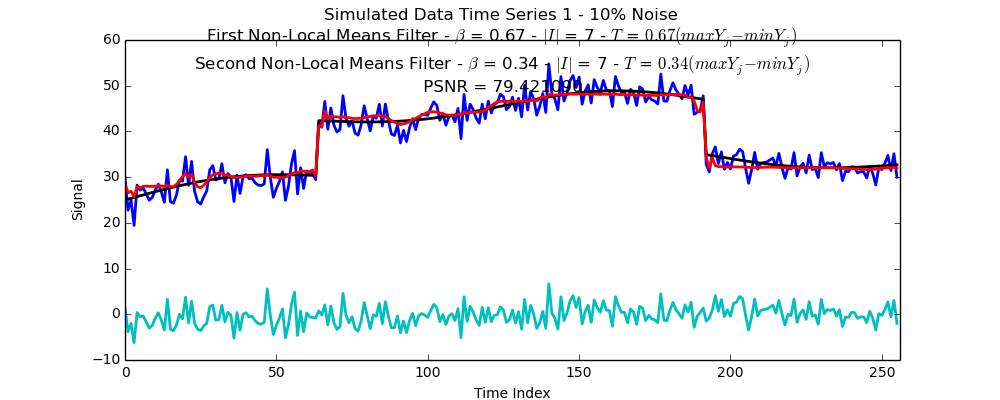
\includegraphics[width = 0.75 \textwidth]{MultiNLMeansSignal1Best.png}
\caption{Non-Local Means Filter - 2 Iterations - Best Denosing with 10\% Noise - Time Series 1}
\label{multinlmeans1best}
\end{figure}

\begin{figure}
\centering
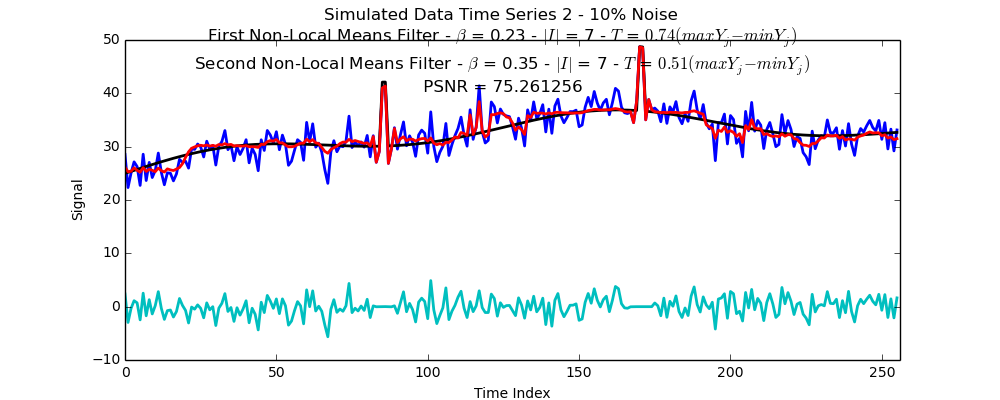
\includegraphics[width = 0.75 \textwidth]{MultiNLMeansSignal2Best.png}
\caption{Non-Local Means Filter - 2 Iterations - Best Denosing with 10\% Noise - Time Series 2}
\label{multinlmeans2best}
\end{figure}

\begin{figure}
\centering
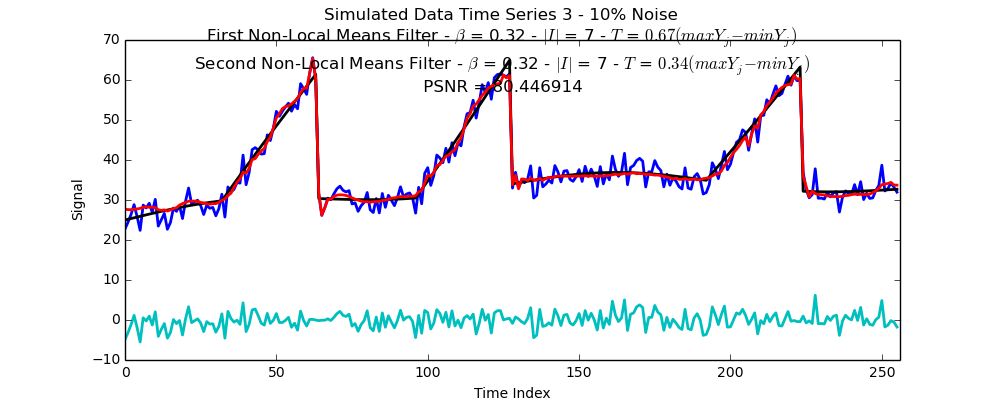
\includegraphics[width = 0.75 \textwidth]{MultiNLMeansSignal3Best.png}
\caption{Non-Local Means Filter - 2 Iterations - Best Denosing with 10\% Noise - Time Series 3}
\label{multinlmeans3best}
\end{figure}

\newpage


\subsubsection{Bilateral Filter and Non-Local Means Filter}

In this last combination, we will consider first using a Bilateral filter and then using a Non-Local Means filter. In order to reduce the number of combinations, we will only consider $\lvert I \rvert = 7$.\\

Using a Bilateral filter before using a Non-Local Means filter appears to make the optimal parameter values for the Non-Local Means filter be more predictable. The optimal values appear to be approximately $\sigma_d = 2.5$, $\sigma_i = 1.6 \hat{\sigma}_n$, $\beta = 0.5$, and $T = 0.9 \left( max Y_j - min Y_j \right) \lvert I \rvert$. The performance of the combination of the Bilateral filter and Non-Local Means filter is better than the performance that either filter independently.

{\footnotesize
\begin{lstlisting}[caption = Time Series 1 - Bilateral Non-Local Means Filter OLS Model, label = {bilateralnlmeans1}]
                            OLS Regression Results                            
==============================================================================
Dep. Variable:                   PSNR   R-squared:                       0.892
Model:                            OLS   Adj. R-squared:                  0.892
Method:                 Least Squares   F-statistic:                     6788.
Date:                Tue, 15 Jul 2014   Prob (F-statistic):               0.00
Time:                        12:16:17   Log-Likelihood:                -10428.
No. Observations:                3300   AIC:                         2.087e+04
Df Residuals:                    3295   BIC:                         2.090e+04
Df Model:                           4                                         
================================================================================
                   coef    std err          t      P>|t|      [95.0% Conf. Int.]
--------------------------------------------------------------------------------
Intercept      102.5001      0.822    124.748      0.000       100.889   104.111
Noise           -1.5519      0.009   -164.547      0.000        -1.570    -1.533
SigD             0.5416      0.074      7.301      0.000         0.396     0.687
SigI             0.2643      0.347      0.762      0.446        -0.416     0.944
I(Beta ** 2)    -1.1556      0.490     -2.359      0.018        -2.116    -0.195
==============================================================================
Omnibus:                      287.471   Durbin-Watson:                   0.381
Prob(Omnibus):                  0.000   Jarque-Bera (JB):               96.439
Skew:                           0.120   Prob(JB):                     1.14e-21
Kurtosis:                       2.198   Cond. No.                         153.
==============================================================================
\end{lstlisting}

\begin{lstlisting}[caption = Time Series 2 - Bilateral Non-Local Means Filter OLS Model, label = {bilateralnlmeans2}]
                            OLS Regression Results                            
==============================================================================
Dep. Variable:                   PSNR   R-squared:                       0.886
Model:                            OLS   Adj. R-squared:                  0.886
Method:                 Least Squares   F-statistic:                     6393.
Date:                Tue, 15 Jul 2014   Prob (F-statistic):               0.00
Time:                        12:16:46   Log-Likelihood:                -10965.
No. Observations:                3300   AIC:                         2.194e+04
Df Residuals:                    3295   BIC:                         2.197e+04
Df Model:                           4                                         
================================================================================
                   coef    std err          t      P>|t|      [95.0% Conf. Int.]
--------------------------------------------------------------------------------
Intercept      104.1532      1.567     66.479      0.000       101.081   107.225
Noise           -1.7739      0.011   -159.825      0.000        -1.796    -1.752
SigD             0.9704      0.476      2.037      0.042         0.037     1.904
SigI            -0.9986      0.377     -2.650      0.008        -1.737    -0.260
I(Beta ** 2)    -1.4782      0.527     -2.806      0.005        -2.511    -0.445
==============================================================================
Omnibus:                     1048.126   Durbin-Watson:                   0.316
Prob(Omnibus):                  0.000   Jarque-Bera (JB):              158.014
Skew:                          -0.074   Prob(JB):                     4.87e-35
Kurtosis:                       1.938   Cond. No.                         240.
==============================================================================
\end{lstlisting}

\begin{lstlisting}[caption = Time Series 3 - Bilateral Non-Local Means Filter OLS Model, label = {bilateralnlmeans3}]
                            OLS Regression Results                            
==============================================================================
Dep. Variable:                   PSNR   R-squared:                       0.945
Model:                            OLS   Adj. R-squared:                  0.945
Method:                 Least Squares   F-statistic:                 1.974e+04
Date:                Tue, 15 Jul 2014   Prob (F-statistic):               0.00
Time:                        12:17:07   Log-Likelihood:                -11405.
No. Observations:                4637   AIC:                         2.282e+04
Df Residuals:                    4632   BIC:                         2.285e+04
Df Model:                           4                                         
================================================================================
                   coef    std err          t      P>|t|      [95.0% Conf. Int.]
--------------------------------------------------------------------------------
Intercept      102.9715      0.533    193.038      0.000       101.926   104.017
Noise           -1.1690      0.004   -279.754      0.000        -1.177    -1.161
SigD            -0.7173      0.215     -3.331      0.001        -1.139    -0.295
SigI            -1.2813      0.050    -25.606      0.000        -1.379    -1.183
I(Beta ** 2)    -3.1488      0.175    -18.031      0.000        -3.491    -2.806
==============================================================================
Omnibus:                      211.138   Durbin-Watson:                   0.972
Prob(Omnibus):                  0.000   Jarque-Bera (JB):              441.138
Skew:                           0.311   Prob(JB):                     1.61e-96
Kurtosis:                       4.377   Cond. No.                         223.
==============================================================================
\end{lstlisting}
}

\begin{figure}
\centering
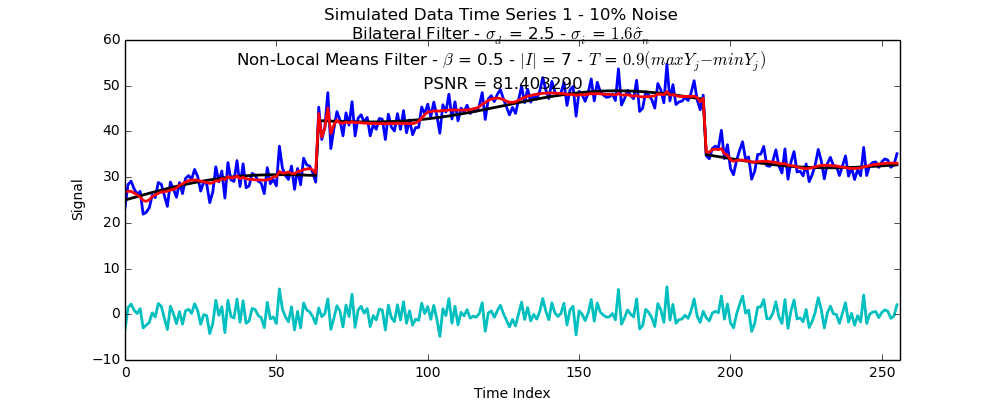
\includegraphics[width = 0.75 \textwidth]{BilateralNLMeansSignal1Best.png}
\caption{Bilateral Non-Local Means Filter - Best Denosing with 10\% Noise - Time Series 1}
\label{bilateralnlmeans1best}
\end{figure}

\begin{figure}
\centering
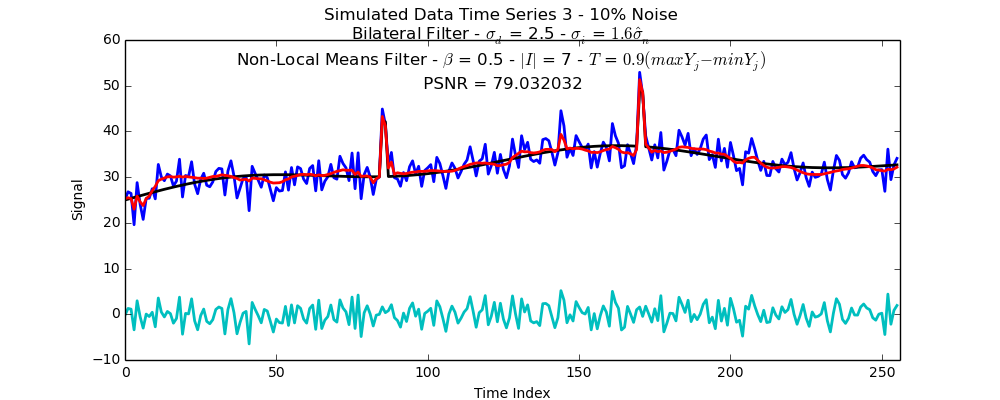
\includegraphics[width = 0.75 \textwidth]{BilateralNLMeansSignal2Best.png}
\caption{Bilateral Non-Local Means Filter - Best Denosing with 10\% Noise - Time Series 2}
\label{bilateralnlmeans2best}
\end{figure}

\begin{figure}
\centering
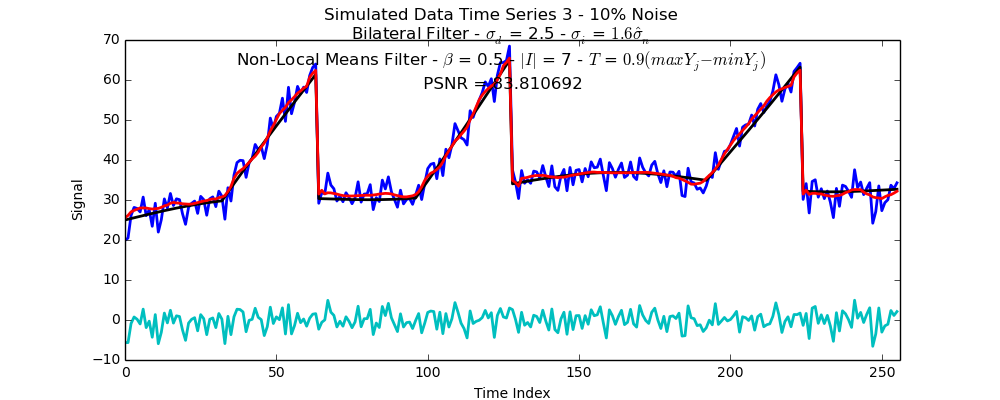
\includegraphics[width = 0.75 \textwidth]{BilateralNLMeansSignal3Best.png}
\caption{Bilateral Non-Local Means Filter - Best Denosing with 10\% Noise - Time Series 3}
\label{bilateralnlmeans3best}
\end{figure}

\newpage


\subsection{Known Time Series with Noise Added - Automatic Parameter Selection}


\subsection{Real World Time Series - Parameter Values from Section 4.1}

In this section we consider real world data that is similar to the three known time series from section 4.1.

\subsubsection{Box Filter}

The Box filter seems to be reasonably effectively on these time series, but it does destroy the peak in the second time series and round the abrupt transitions in the first time series.

\begin{figure}
\centering
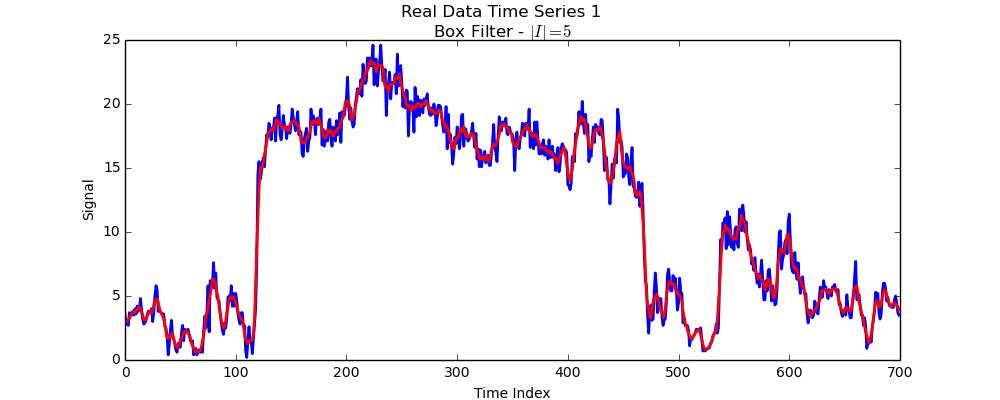
\includegraphics[width = 0.75 \textwidth]{BoxRealSignal1.png}
\caption{Box Filter - Real Data - Time Series 1}
\label{boxrealsignal1}
\end{figure}

\begin{figure}
\centering
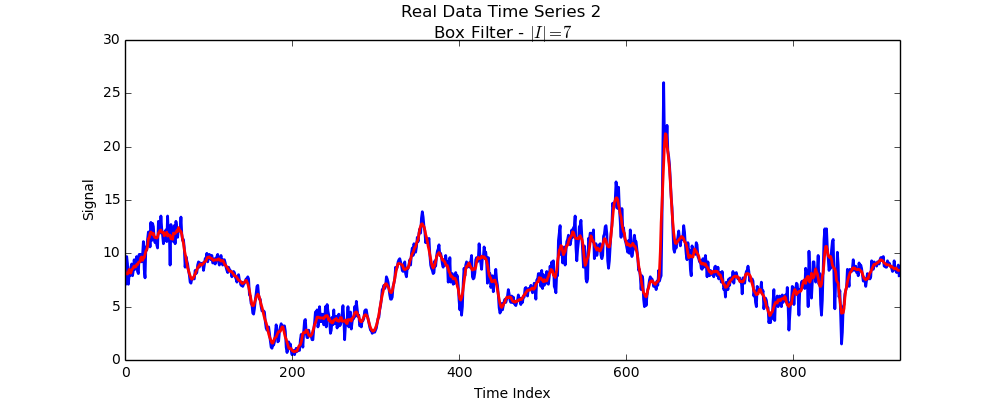
\includegraphics[width = 0.75 \textwidth]{BoxRealSignal2.png}
\caption{Box Filter - Real Data - Time Series 2}
\label{boxrealsignal2}
\end{figure}

\begin{figure}
\centering
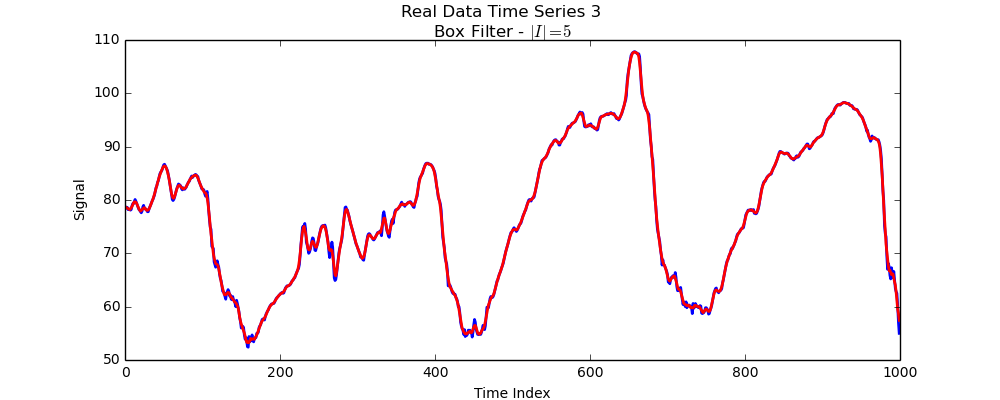
\includegraphics[width = 0.75 \textwidth]{BoxRealSignal3.png}
\caption{Box Filter - Real Data - Time Series 3}
\label{boxrealsignal3}
\end{figure}

\newpage

\subsubsection{Gaussian Filter}

Similarly, the Gaussian filter seems to be reasonably effectively on these time series, but it does destroy the peak in the second time series and round the abrupt transitions in the first time series.

\begin{figure}
\centering
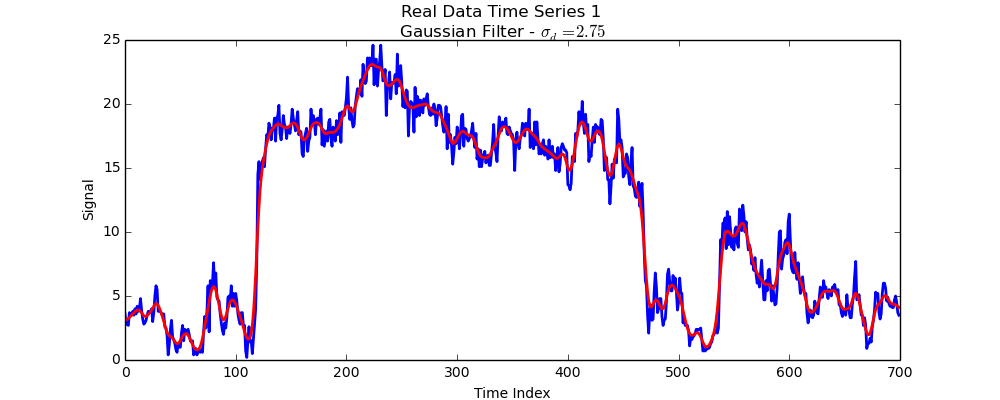
\includegraphics[width = 0.75 \textwidth]{GaussianRealSignal1.png}
\caption{Gaussian Filter - Real Data - Time Series 1}
\label{gaussianrealsignal1}
\end{figure}

\begin{figure}
\centering
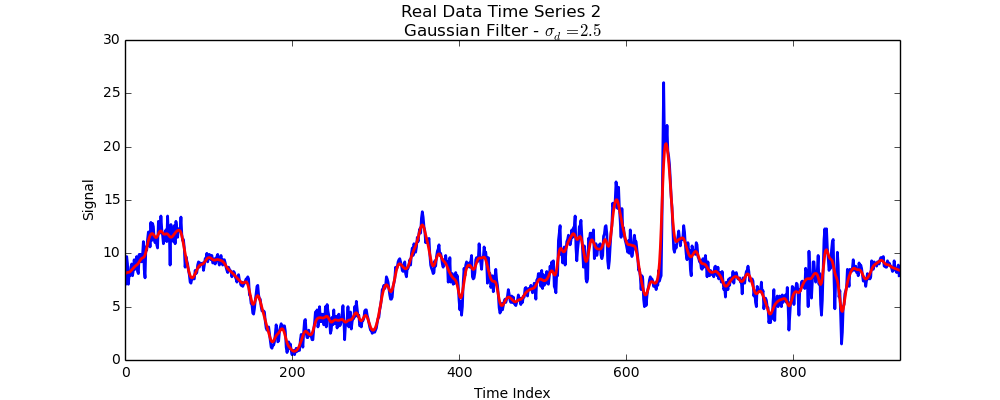
\includegraphics[width = 0.75 \textwidth]{GaussianRealSignal2.png}
\caption{Gaussian Filter - Real Data - Time Series 2}
\label{gaussianrealsignal2}
\end{figure}

\begin{figure}
\centering
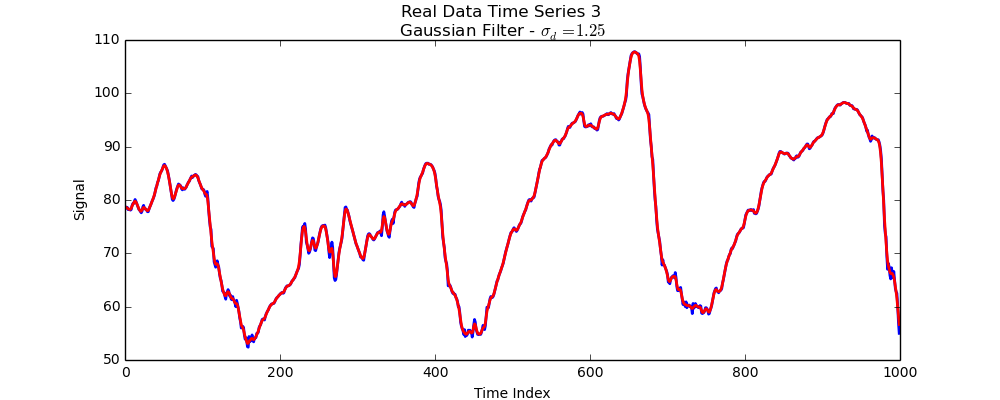
\includegraphics[width = 0.75 \textwidth]{GaussianRealSignal3.png}
\caption{Gaussian Filter - Real Data - Time Series 3}
\label{gaussianrealsignal3}
\end{figure}

\newpage

\subsubsection{Bilateral Filter}

The Bilateral filter seems to be very effectively on these time series, and it does not destroy the peak in the second time series or round the abrupt transitions in the first time series.

\begin{figure}
\centering
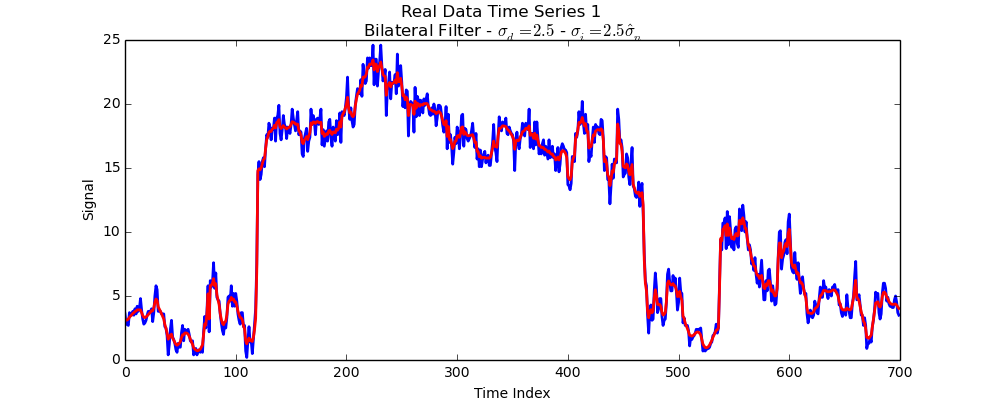
\includegraphics[width = 0.75 \textwidth]{BilateralRealSignal1.png}
\caption{Bilateral Filter - Real Data - Time Series 1}
\label{bilateralrealsignal1}
\end{figure}

\begin{figure}
\centering
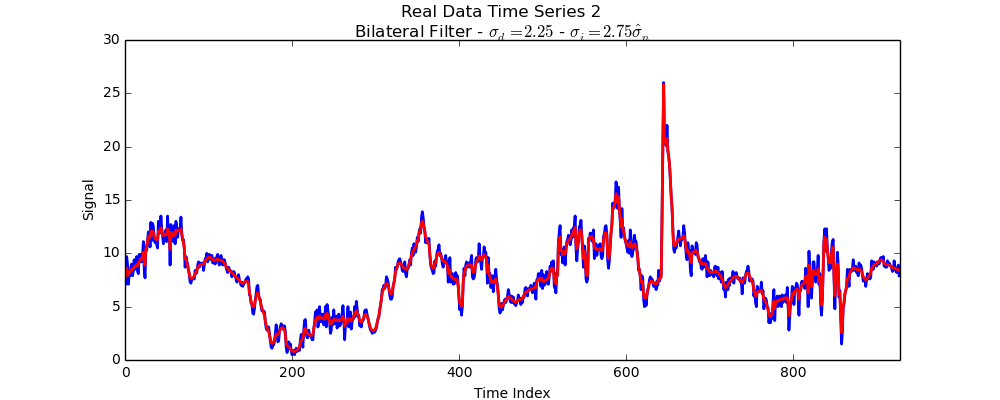
\includegraphics[width = 0.75 \textwidth]{BilateralRealSignal2.png}
\caption{Bilateral Filter - Real Data - Time Series 2}
\label{bilateralrealsignal2}
\end{figure}

\begin{figure}
\centering
\includegraphics[width = 0.75 \textwidth]{BilateralRealSignal3.png}
\caption{Bilateral Filter - Real Data - Time Series 3}
\label{bilateralrealsignal3}
\end{figure}

\newpage

\subsubsection{Fast Fourier Transform Coefficient Thresholding}

Fast Fourier Transform coefficient thresholding does not seem to be removing enough of the noise in these time series with the thresholds from section 4.1.

\begin{figure}
\centering
\includegraphics[width = 0.75 \textwidth]{FFTRealSignal1.png}
\caption{Fast Fourier Transform Coefficient Thresholding - Real Data - Time Series 1}
\label{fftrealsignal1}
\end{figure}

\begin{figure}
\centering
\includegraphics[width = 0.75 \textwidth]{FFTRealSignal2.png}
\caption{Fast Fourier Transform Coefficient Thresholding - Real Data - Time Series 2}
\label{fftrealsignal2}
\end{figure}

\begin{figure}
\centering
\includegraphics[width = 0.75 \textwidth]{FFTRealSignal3.png}
\caption{Fast Fourier Transform Coefficient Thresholding - Real Data - Time Series 3}
\label{fftrealsignal3}
\end{figure}

\newpage

\subsubsection{Wavelet Transform Coefficient Thresholding}

Similarly, the Wavelet Transform coefficient thresholding does not seem to be removing enough of the noise in these time series with the thresholds from section 4.1.

\begin{figure}
\centering
\includegraphics[width = 0.75 \textwidth]{WaveletRealSignal1.png}
\caption{Wavelet Transform Coefficient Thresholding - Real Data - Time Series 1}
\label{waveletrealsignal1}
\end{figure}

\begin{figure}
\centering
\includegraphics[width = 0.75 \textwidth]{WaveletRealSignal2.png}
\caption{Wavelet Transform Coefficient Thresholding - Real Data - Time Series 2}
\label{waveletrealsignal2}
\end{figure}

\begin{figure}
\centering
\includegraphics[width = 0.75 \textwidth]{WaveletRealSignal3.png}
\caption{Wavelet Transform Coefficient Thresholding - Real Data - Time Series 3}
\label{waveletrealsignal3}
\end{figure}

\newpage

\subsubsection{Non-Local Means Filter}

Also, the Non-Local Means filter seems to be removing insufficient noise from the time series.

\begin{figure}
\centering
\includegraphics[width = 0.75 \textwidth]{NLMeansRealSignal1.png}
\caption{Non-Local Means Filter - Real Data - Time Series 1}
\label{nlmeansrealsignal1}
\end{figure}

\begin{figure}
\centering
\includegraphics[width = 0.75 \textwidth]{NLMeansRealSignal2.png}
\caption{Non-Local Means Filter - Real Data - Time Series 2}
\label{nlmeansrealsignal2}
\end{figure}

\begin{figure}
\centering
\includegraphics[width = 0.75 \textwidth]{NLMeansRealSignal3.png}
\caption{Non-Local Means Filter - Real Data - Time Series 3}
\label{nlmeansrealsignal3}
\end{figure}

\newpage

\subsubsection{Iterated Bilateral Filter}

The iterated Bilateral filters seem to be reasonably effectively but there does not seem to be a significant difference between the performance of the Bilateral filter and the iterated Bilateral filter. Also, the inconsistent optimized  parameters makes the iterated Bilateral filter difficult to use in practice.

\paragraph{Same Parameters - Two Iterations}

\begin{figure}
\centering
\includegraphics[width = 0.75 \textwidth]{2SameBilateralRealSignal1.png}
\caption{Bilateral Filter - 2 Same Iterations - Real Data - Time Series 1}
\label{2samebilateralrealsignal1}
\end{figure}

\begin{figure}
\centering
\includegraphics[width = 0.75 \textwidth]{2SameBilateralRealSignal2.png}
\caption{Bilateral Filter - 2 Same Iterations - Real Data - Time Series 2}
\label{2samebilateralrealsignal2}
\end{figure}

\begin{figure}
\centering
\includegraphics[width = 0.75 \textwidth]{2SameBilateralRealSignal3.png}
\caption{Bilateral Filter - 2 Same Iterations - Real Data - Time Series 3}
\label{2samebilateralrealsignal3}
\end{figure}

\newpage

\paragraph{Same Parameters - Iterated to Tolerance}

\begin{figure}
\centering
\includegraphics[width = 0.75 \textwidth]{ItrSameBilateralRealSignal1.png}
\caption{Bilateral Filter - Multiple Iterations - Real Data - Time Series 1}
\label{itrsamebilateralrealsignal1}
\end{figure}

\begin{figure}
\centering
\includegraphics[width = 0.75 \textwidth]{ItrSameBilateralRealSignal2.png}
\caption{Bilateral Filter - Multiple Iterations - Real Data - Time Series 2}
\label{itrsamebilateralrealsignal2}
\end{figure}

\begin{figure}
\centering
\includegraphics[width = 0.75 \textwidth]{ItrSameBilateralRealSignal3.png}
\caption{Bilateral Filter - Multiple Iterations - Real Data - Time Series 3}
\label{itrsamebilateralrealsignal3}
\end{figure}

\newpage

\paragraph{Different Parameters - Two Iterations}

\begin{figure}
\centering
\includegraphics[width = 0.75 \textwidth]{2DiffBilateralRealSignal1.png}
\caption{Bilateral Filter - 2 Different Iterations - Real Data - Time Series 1}
\label{2diffbilateralrealsignal1}
\end{figure}

\begin{figure}
\centering
\includegraphics[width = 0.75 \textwidth]{2DiffBilateralRealSignal2.png}
\caption{Bilateral Filter - 2 Different Iterations - Real Data - Time Series 2}
\label{2diffbilateralrealsignal2}
\end{figure}

\begin{figure}
\centering
\includegraphics[width = 0.75 \textwidth]{2DiffBilateralRealSignal3.png}
\caption{Bilateral Filter - 2 Different Iterations - Real Data - Time Series 3}
\label{2diffbilateralrealsignal3}
\end{figure}

\newpage

\subsubsection{Iterated Non-Local Means Filter}

The iterated Non-Local Means filter removed more of the noise than a single application of the Non-Local Means filter; however, two iterations of the Non-Local Means filter takes a significant amount of time to run. Also, the inconsistent optimized  parameters makes the iterated Non-Local Means filter difficult to use in practice.

\begin{figure}
\centering
\includegraphics[width = 0.75 \textwidth]{MultiNLMeansRealSignal1.png}
\caption{Non-Local Means Filter - 2 Iterations - Real Data - Time Series 1}
\label{multinlmeansrealsignal1}
\end{figure}

\begin{figure}
\centering
\includegraphics[width = 0.75 \textwidth]{MultiNLMeansRealSignal2.png}
\caption{Non-Local Means Filter - 2 Iterations - Real Data - Time Series 2}
\label{multinlmeansrealsignal2}
\end{figure}

\begin{figure}
\centering
\includegraphics[width = 0.75 \textwidth]{MultiNLMeansRealSignal3.png}
\caption{Non-Local Means Filter - 2 Iterations - Real Data - Time Series 3}
\label{multinlmeansrealsignal3}
\end{figure}

\newpage

\subsubsection{Bilateral Filter and Non-Local Means Filter}

Combining the Bilateral and Non-Local Means filters appears to be more effective that either the Bilateral filter or Non-Local Means filter alone, and the optimal parameters are more consistent than of the Non-Local Means filter alone. Also, with the speed of the Bilateral filter, denoising with the combination of the Bilateral and Non-Local Means filters is not significantly slower than the Non-Local Means filter.

\begin{figure}
\centering
\includegraphics[width = 0.75 \textwidth]{BilateralNLMeansRealSignal1.png}
\caption{Bilateral Non-Local Means Filter - Real Data - Time Series 1}
\label{bilateralmultinlmeansrealsignal1}
\end{figure}

\begin{figure}
\centering
\includegraphics[width = 0.75 \textwidth]{BilateralNLMeansRealSignal2.png}
\caption{Bilateral Non-Local Means Filter - Real Data - Time Series 2}
\label{bilateralmultinlmeansrealsignal2}
\end{figure}

\begin{figure}
\centering
\includegraphics[width = 0.75 \textwidth]{BilateralNLMeansRealSignal3.png}
\caption{Bilateral Non-Local Means Filter - Real Data - Time Series 3}
\label{bilateralmultinlmeansrealsignal3}
\end{figure}

\newpage


\subsection{Real World Time Series - Automatic Parameter Selection}


\section{Conclusions}


Technique Situations

Parameter Selection and Optimization

Real Time Implementation

Quality Assessment


\FloatBarrier

%\bibliographystyle{acm}
\bibliographystyle{plain}
\bibliography{notes}  
\pagebreak

\appendix

\section{Summary of Denoising Techniques}

\subsection{Box Filter}

\begin{displaymath}
s_i = \sum _{i \in I} w \left(i, j \right) y_j
\end{displaymath}

\noindent
where the weights are given by the function

\begin{displaymath}
w\left(i, j\right) = \frac{1}{\lvert I \rvert}
\end{displaymath}

\noindent
$I$ is the interval, or window, of the filter


\subsection{Gaussian Filter}

\begin{displaymath}
s_i = \sum _{i \in I} w \left(i, j \right) y_j
\end{displaymath}

\noindent
where the weights are given by the function

\begin{displaymath}
w\left(i, j\right) = \frac{1}{z_i} \frac{1}{\sqrt{2 \pi} \sigma_d} e^{-\frac{\lvert i - j \rvert}{2 \sigma_d^2}}
\end{displaymath}

\noindent
$z_i$ is a normalization factor


\subsection{Bilateral Filter}

\begin{displaymath}
s_i = \sum _{i \in I} w \left(i, j \right) y_j
\end{displaymath}

\noindent
where the weights are given by the function

\begin{displaymath}
w\left(i, j\right) = \frac{1}{z_i} \frac{1}{2 \pi \sigma_d \sigma_i} e^{-\frac{\lvert i - j \rvert}{2 \sigma_d^2}}e^{-\frac{\lvert y_i - y_j \rvert}{2 \sigma_i^2}}
\end{displaymath}

\noindent
$z_i$ is a normalization factor

\noindent
Optimal values for $\sigma_d$ appear to be in the range $\left[ 2.0, 3.0 \right]$ and optimal values for $\sigma_i$ appear to be in range $\left[ 2.0 \hat{\sigma}_n, 3.0 \hat{\sigma}_n \right]$.


\subsection{Fast Fourier Transform Coefficient Thresholding}

$v\left(\alpha\right)$ represents the transformed data, the frequency coefficients

\begin{displaymath}
v\left(\alpha\right) = 
\begin{cases}
v\left(\alpha\right) & \lvert v\left(\alpha\right)\rvert > \mu \\
0 & \lvert v\left(\alpha\right)\rvert < \mu
\end{cases}
\end{displaymath}


\subsection{Wavelet Transform Coefficient Thresholding}

$v\left(\alpha\right)$ represents the transformed data, the frequency coefficients

\begin{displaymath}
v\left(\alpha\right) = 
\begin{cases}
v\left(\alpha\right) & \lvert v\left(\alpha\right)\rvert > \mu \\
0 & \lvert v\left(\alpha\right)\rvert < \mu
\end{cases}
\end{displaymath}


\subsection{Non-Local Means Filter}

\begin{displaymath}
s_i = \sum _{i \in N} w \left(i, j \right) y_j
\end{displaymath}

\noindent
where the weights are given by the function

\begin{displaymath}
w\left(i, j\right) = 
\begin{cases}
\frac{1}{z_i} e^{-\frac{\lvert Y_i - Y_j \rvert ^2}{2 \beta \hat{\sigma}^2_n \lvert Y \rvert}} & \lvert Y_i - Y_j \rvert < T \\
0 & $otherwise$
\end{cases}
\end{displaymath}


\pagebreak


\section{Box Filter}

\begin{lstlisting}[language = Python]

# --------------------------------------------------
# Title: BoxFilter1D.py
# Date: 24 June 2014
# Author: Jeremy L Thompson
# Purpose: Implement Box Filter on 1D data
# --------------------------------------------------


import numpy as np


# ---- Data Input ----

# Read data into a matrix
arr = []
f = open("2010_10_gen.txt","r")
for line in f.readlines():
    numbers = line.strip().split('\t')
    arr.append(numbers)

# Transpose the matrix
transArr = []
transArr = [list(col) for col in zip(*arr)]

# Extract the 4th (data) row
Data = []
Data = [int(i) for i in transArr[3][1:]]

DataLen = len(Data)


# ---- Set Up Moving Aveage ----

# Get the Moving Average length
window = int(raw_input("Please enter the number of terms to average (odd number): "))

halfwindow = (window - 1)/2

BoxFilter = np.ones(window)/window


# ---- Filter the Data ----

SmoothedData = np.zeros(len(Data))

# Left Hand Side
for i in range(0, halfwindow):
    SmoothedData[i] = np.sum(Data[0 : i + halfwindow + 1])/(i + halfwindow + 1)

# Middle
for i in  range(halfwindow, DataLen - halfwindow):
    SmoothedData[i] = np.dot(Data[i - halfwindow : i + halfwindow + 1], BoxFilter)

# Right Hand Side
for i in range(DataLen - halfwindow, DataLen):
    SmoothedData[i] = np.sum(Data[i - halfwindow : DataLen])/(DataLen - i + halfwindow)


# ---- Results ----

# Plotting results
import matplotlib.pyplot as plt

plt.title('Actual Data vs Smoothed Data',  fontsize = 22)
plt.xlabel('Time Index')
plt.ylabel('Wind Power Generated')

plt.plot(range(len(Data)), Data, 'k', lw = 3)
plt.plot(range(len(SmoothedData)), SmoothedData, 'b')

plt.show()

Noise = SmoothedData - Data

plt.title('Calculated Noise',  fontsize = 22)
plt.xlabel('Time Index')
plt.ylabel('Calculated Noise')

plt.plot(range(DataLen), Noise, 'b')

print 'Noise Mean: ' + str(np.average(Noise))
print 'Noise Std Dev: ' + str(np.std(Noise))

plt.show()


# ---- Loop for Updating Smoothed Data ----
'''
# Note: this would be run when a new data point is received (rather than re-running the whole function for all data)

SmoothedData.append(sum(Data[len(Data) - halfwindow : len(Data))/(halfwindow + 1)))

for i in range(len(Data) - halfwindow - 1, len(Data) - 1):
   SmoothedData[i] = sum(Data[i - halfwindow : len(Data)])/(len(Data) - 1 - i + halfwindow)
'''

\end{lstlisting}

\pagebreak


\section{Gaussian Filter Code}

\begin{lstlisting}[language = Python]

# --------------------------------------------------
# Title: GaussianFilter1D.py
# Date: 24 June 2014
# Author: Jeremy L Thompson
# Purpose: Implement Gaussian Filter on 1D data
# --------------------------------------------------


import numpy as np


# ---- Data Input ----

# Read data into a matrix
arr = []
f = open("2010_10_gen.txt","r")
for line in f.readlines():
    numbers = line.strip().split('\t')
    arr.append(numbers)

# Transpose the matrix
transArr = []
transArr = [list(col) for col in zip(*arr)]

# Extract the 4th (data) row
Data = []
Data = [int(i) for i in transArr[3][1:]]

DataLen = len(Data)


# ---- Set up Gaussian Filter ----

def varest(Data):
    DataLen = len(Data)

    varest = 0.0

    for i in range(1, DataLen - 1):
        varest += (0.5*Data[i - 1] - Data[i] + 0.5*Data[i + 1])**2

    varest *= 2.0/(3.0*(DataLen - 2))

    return varest

# Get the sigma

print 'The estimated noise standard deviation is ' + str(varest(Data)**(1/2))

sigma = float(raw_input("Please enter the desired spatial kernel standard deviation: "))

# Define Gaussian Function
def gaussian(x, sigma):
    return 1/(np.sqrt(2*np.pi)*sigma)*np.exp(-np.power(x, 2.)/(2*np.power(sigma, 2.)))

# Build Gaussian Filter
filtersize = 2*int(5*sigma) + 1
filtersize = min(filtersize, DataLen - 1) # prevent overrun

offset = (filtersize - 1)/2

Filter = np.linspace(-offset, offset, filtersize)
Filter = gaussian(Filter, sigma)
Filter = Filter/np.sum(Filter) # Normalize


# ---- Filter the Data ----

# Set Up Output
SmoothedData = np.array(np.zeros(DataLen))

# Left Hand Side
for i in range(0, offset):
    SmoothedData[i] = np.dot(Data[0 : i + offset + 1], Filter[offset - i : filtersize]/np.sum(Filter[offset - i : filtersize]))

# Middle
for i in range(offset, DataLen - offset):
    SmoothedData[i] = np.dot(Data[i - offset : i + offset + 1], Filter)

# Right Hand Side
for i in range(DataLen - offset, DataLen):
    SmoothedData[i] = np.dot(Data[i - offset : DataLen], Filter[0 : filtersize - offset - i + DataLen - 1]/np.sum(Filter[0 : filtersize - offset - i + DataLen - 1]))


# ---- Results ----

# Plotting results
import matplotlib.pyplot as plt

plt.title('Actual Data vs Smoothed Data',  fontsize = 22)
plt.xlabel('Time Index')
plt.ylabel('Wind Power Generated')

plt.plot(range(DataLen), Data, 'k', lw = 3)
plt.plot(range(DataLen), SmoothedData, 'b')

plt.show()

Noise = SmoothedData - Data

plt.title('Calculated Noise',  fontsize = 22)
plt.xlabel('Time Index')
plt.ylabel('Calculated Noise')

plt.plot(range(DataLen), Noise, 'b')

print 'Noise Mean: ' + str(np.average(Noise))
print 'Noise Std Dev: ' + str(np.std(Noise))

plt.show()


# ---- Loop for Updating Smoothed Data ----
'''
# Note: this would be run when a new data point is received (rather than re-running the whole function for all data)

SmoothedData.append(sum(np.multiply(Data[DataLen - offset - 1 : DataLen], Filter[0 : offset]/sum(Filter[0 : offset]))))

for i in range(DataLen - offset - 1, DataLen - 1):
    SmoothedData[i] = sum(np.multiply(Data[i - offset - 1 : DataLen], Filter[0 : filtersize - offset - i + DataLen]/sum(Filter[0 : filtersize - offset - i +DataLen])))
'''

\end{lstlisting}

\pagebreak


\section{Bilateral Filter Code}

\begin{lstlisting}[language = Python]

# --------------------------------------------------
# Title: BilateralFilter1D.py
# Date: 24 June 2014
# Author: Jeremy L Thompson
# Purpose: Implement Bilateral Filter on 1D data
# --------------------------------------------------


import numpy as np


# ---- Data Input ----

# Read data into a matrix
arr = []
f = open("2010_10_gen.txt","r")
for line in f.readlines():
    numbers = line.strip().split('\t')
    arr.append(numbers)

# Transpose the matrix
transArr = []
transArr = [list(col) for col in zip(*arr)]

# Extract the 4th (data) row
Data = []
Data = np.array([int(i) for i in transArr[3][1:]])

DataLen = len(Data)


# ---- Set up Gaussian Filter ----

def varest(Data):
    DataLen = len(Data)

    varest = 0

    for i in range(1, DataLen - 1):
        varest += (0.5*Data[i - 1] - Data[i] + 0.5*Data[i + 1])**2

    varest *= 2./(3.*float(DataLen - 2))

    return varest

# Get the sigmas

print 'The estimated noise standard deviation is ' + str(np.sqrt(varest(Data)))

sigmadist = float(raw_input("Please enter the desired spatial kernel standard deviation: "))

sigmaint = float(raw_input("Please enter the desired intensity kernel standard deviation: "))

# Define Gaussian Function
def gaussian(x, sigma):
    return 1/((2*np.pi)**0.5*sigma)*np.exp(-x**2./(2*sigma**2.))

# Build Gaussian Filter
filtersize = 2*int(5*sigmadist) + 1
filtersize = min(filtersize, DataLen - 1) # prevent overrun

offset = (filtersize - 1)/2

SpatialFilter = np.linspace(-offset, offset, filtersize)
SpatialFilter = gaussian(SpatialFilter, sigmadist)
SpatialFilter *= 1/np.sum(SpatialFilter) # Normalize


# ---- Filter the Data ----

# Set Up Output
SmoothedData = np.zeros(DataLen)

IntensityFilter = np.array([])

# Left Hand Side
for i in range(0, offset):
    # Update Intensity Filter
    IntensityFilter = Data[0 : i + offset + 1] - Data[i]
    IntensityFilter = gaussian(IntensityFilter, sigmaint)
    IntensityFilter = np.multiply(IntensityFilter, SpatialFilter[offset - i : filtersize])
    IntensityFilter *= 1/np.sum(IntensityFilter) # Normalize

    # Smooth Next Data Point
    SmoothedData[i] = np.dot(Data[0 : i + offset + 1], IntensityFilter)

# Middle
for i in range(offset, DataLen - offset):
    # Update Intensity Filter
    IntensityFilter = Data[i - offset : i + offset + 1] - Data[i]
    IntensityFilter = gaussian(IntensityFilter, sigmaint)
    IntensityFilter = np.multiply(IntensityFilter, SpatialFilter)
    IntensityFilter *= 1/np.sum(IntensityFilter) # Normalize

    # Smooth Next Data Point
    SmoothedData[i] = np.dot(Data[i - offset : i + offset + 1], IntensityFilter)

# Right Hand Side
for i in range(DataLen - offset, DataLen):
    # Update Intensity Filter
    IntensityFilter = Data[i - offset : DataLen] - Data[i]
    IntensityFilter = gaussian(IntensityFilter, sigmaint)
    IntensityFilter = np.multiply(IntensityFilter, SpatialFilter[0 : filtersize - (i - DataLen + offset) - 1])
    IntensityFilter *= 1/np.sum(IntensityFilter) # Normalize

    # Smooth Next Data Point
    SmoothedData[i] = np.dot(Data[i - offset : DataLen], IntensityFilter)


# ---- Results ----

# Plotting results
import matplotlib.pyplot as plt

plt.title('Actual Data vs Smoothed Data',  fontsize = 22)
plt.xlabel('Time Index')
plt.ylabel('Wind Power Generated')

plt.plot(range(DataLen), Data, 'k', lw = 3)
plt.plot(range(len(SmoothedData)), SmoothedData, 'b')

plt.show()

Noise = SmoothedData - Data

plt.title('Calculated Noise',  fontsize = 22)
plt.xlabel('Time Index')
plt.ylabel('Calculated Noise')

plt.plot(range(DataLen), Noise, 'b')

print 'Noise Mean: ' + str(np.average(Noise))
print 'Noise Std Dev: ' + str(np.std(Noise))

plt.show()


# ---- Loop for Updating Smoothed Data ----
'''
 Note: this would be run when a new data point is received (rather than re-running the whole function for all data)

# Update Intensity Filter
IntensityFilter = Data[i - offset : DataLen] - Data[i]
IntensityFilter = gaussian(IntensityFilter, sigmaint)
IntensityFilter = np.multiply(IntensityFilter, SpatialFilter[0 : filtersize - (i - DataLen + offset) - 1])
IntensityFilter *= 1/sum(IntensityFilter) # Normalize

# Smooth Next Data Point
SmoothedData.append(np.dot(Data[i - offset : DataLen], IntensityFilter)

for i in range(DataLen - offset - 1, DataLen - 1):
    # Update Intensity Filter
    IntensityFilter = Data[i - offset : DataLen] - Data[i]
    IntensityFilter = gaussian(IntensityFilter, sigmaint)
    IntensityFilter = np.multiply(IntensityFilter, SpatialFilter[0 : filtersize - (i - DataLen - 1 + offset) - 1])
    IntensityFilter *= 1/sum(IntensityFilter) # Normalize

    # Smooth Next Data Point
    SmoothedData[i] = np.dot(Data[i - offset : DataLen], IntensityFilter)
'''

\end{lstlisting}

\pagebreak

\section{Fast Fourier Transform Code}

\begin{lstlisting}[language = Python]
# --------------------------------------------------
# Title: FFTFilter1D.py
# Date: 10 June 2014
# Author: Jeremy L Thompson
# Purpose: Implement FFT Hard Filter on 1D data
# --------------------------------------------------


import numpy as np


# ---- Data Input ----

# Read data into a matrix
arr = []
f = open("2010_10_gen.txt","r")
for line in f.readlines():
    numbers = line.strip().split('\t')
    arr.append(numbers)

# Transpose the matrix
transArr = []
transArr = [list(col) for col in zip(*arr)]

# Extract the 4th (data) row
Data = []
Data = [int(i) for i in transArr[3][1:]]

DataLen = len(Data)

# Pad Data to power of 2
pad = 2
while pad < DataLen:
    pad *= 2

Data = np.append(Data, np.zeros(pad - DataLen))

OldDataLen = DataLen
DataLen = len(Data)

datamean = np.average(Data)

Data -= datamean

# Get the threshold

thresh = float(raw_input("Please enter the desired FFT threshold: "))

# ---- Slow DFT ----

def SFT(x):
    N = len(x)
    n = np.arange(N)
    k = n.reshape((N, 1))

    coeffs = np.exp(-2j*np.pi*k*n/N)

    return np.dot(coeffs, x)


# ---- Fast DFT ----

def FFT(x):
    N = len(x)

    if N % 2 > 0 or N <= 32:
        return SFT(x)
    else:
        X_even = FFT(x[ : : 2])
        X_odd = FFT(x[1 : : 2])
        factor = np.exp(-2j*np.pi*np.arange(N)/N)

        return np.concatenate([X_even + factor[ : N/2]*X_odd, X_even + factor[N/2 : ]*X_odd])


# ---- Slow iDFT ----

def iSFT(x):
    N = len(x)
    n = np.arange(N)
    k = n.reshape((N, 1))

    coeffs = np.exp(2j*np.pi*k*n/N)

    return np.dot(coeffs, x)


# ---- Fast iDFT ----

def iFFT(x, initial):
    N = len(x)

    if N % 2 > 0 or N <= 32:
        output = iSFT(x)
    else:
        X_even = iFFT(x[ : : 2], False)
        X_odd = iFFT(x[1 : : 2], False)
        factor = np.exp(2j*np.pi*np.arange(N)/N)

        output = np.concatenate([X_even + factor[ : N/2]*X_odd, X_even + factor[N/2 : ]*X_odd])

    if initial == True:
        output /= N
        return output
    else:
        return output


# ---- FFT Data ----

FTData = FFT(Data)


# ---- Smooth Data ----

hardcut = thresh*np.std(FTData)

for i in range(DataLen):
    if np.abs(FTData[i]) < hardcut:
        FTData[i] = 0


# ---- Inverse FFT Data ----

SmoothedData = np.real(iFFT(FTData, True))


# ---- Results ----

# Plotting results

import matplotlib.pyplot as plt

plt.title('Actual Data vs Smoothed Data',  fontsize = 22)
plt.xlabel('Time Index')
plt.ylabel('Wind Power Generated')

plt.plot(range(OldDataLen), Data[0 : OldDataLen] + datamean, 'k', lw = 3)
plt.plot(range(OldDataLen), SmoothedData[0 : OldDataLen] + datamean, 'b')

plt.show()

Noise = SmoothedData - Data

plt.title('Calculated Noise',  fontsize = 22)
plt.xlabel('Time Index')
plt.ylabel('Calculated Noise')

plt.plot(range(OldDataLen), Noise[0 : OldDataLen], 'b')

print 'Noise Mean: ' + str(np.average(Noise))
print 'Noise Std Dev: ' + str(np.std(Noise))

plt.show()
\end{lstlisting}

\pagebreak


\section{Harr Wavelets Code}

\begin{lstlisting}[language = Python]

# --------------------------------------------------
# Title: WaveletFilter1D.py
# Date: 10 June 2014
# Author: Jeremy L Thompson
# Purpose: Implement Wavelet Hard Thresholding
#          Filter on 1D data
# --------------------------------------------------


import numpy as np


# ---- Data Input ----

# Read data into a matrix
arr = []
f = open("2010_10_gen.txt","r")
for line in f.readlines():
    numbers = line.strip().split('\t')
    arr.append(numbers)

# Transpose the matrix
transArr = []
transArr = [list(col) for col in zip(*arr)]

# Extract the 4th (data) row
Data = []
Data = [int(i) for i in transArr[3][1:]]

DataLen = len(Data)

datamean = np.average(Data)

Data -= datamean


# Get the threshold

thresh = float(raw_input("Please enter the desired wavelet threshold: "))


# ---- DWT ----

def DWT(x):
    N = len(x)

    if N == 1 or N % 2 > 0:
        return x, N

    output = np.zeros(N)

    for i in range(N/2):
        output[i] = (x[i*2] + x[i*2 + 1])/2.
        output[N/2 + i] = (x[i*2] - x[i*2 + 1])/2.

    output[0 : N/2], length = DWT(output[0 : N/2])

    return output, length


# ---- iDWT ----

def iDWT(x, p, length):
    N = len(x)
    cap = 2**p*length

    if cap == N:
        return x

    output = np.zeros(N)
    output[2*cap : N] = x[2*cap : N]

    for i in range(cap):
        output[2*i] = x[i] + x[cap + i]
        output[2*i + 1] = x[i] - x[cap + i]

    output = iDWT(output, p + 1, length)

    return output


# ---- DWT Data ----

WTData, length = DWT(Data)


# ---- Smooth Data ----

hardcut = thresh*np.std(WTData)

for i in range(DataLen):
    if np.abs(WTData[i]) < hardcut:
        WTData[i] = 0


# ---- Inverse DWT Data ----

SmoothedData = iDWT(WTData, 0, length)


# ---- Results ----

# Plotting results

import matplotlib.pyplot as plt

plt.title('Actual Data vs Smoothed Data',  fontsize = 22)
plt.xlabel('Time Index')
plt.ylabel('Wind Power Generated')

plt.plot(range(DataLen), Data + datamean, 'k', lw = 3)
plt.plot(range(DataLen), SmoothedData + datamean, 'b')

plt.show()

Noise = SmoothedData - Data

plt.title('Calculated Noise',  fontsize = 22)
plt.xlabel('Time Index')
plt.ylabel('Calculated Noise')

plt.plot(range(DataLen), Noise, 'b')

print 'Noise Mean: ' + str(np.average(Noise))
print 'Noise Std Dev: ' + str(np.std(Noise))

plt.show()

\end{lstlisting}

\pagebreak


\section{Non-Local Means Code}

\begin{lstlisting}[language = Python]

# --------------------------------------------------
# Title: NLMeansFilter1D.py
# Date: 24 June 2014
# Author: Jeremy L Thompson
# Purpose: Implement NL Means Filter on 1D data
# --------------------------------------------------


import numpy as np


# ---- Data Input ----

# Read data into a matrix
arr = []
f = open("2010_10_gen.txt","r")
for line in f.readlines():
    numbers = line.strip().split('\t')
    arr.append(numbers)

# Transpose the matrix
transArr = []
transArr = [list(col) for col in zip(*arr)]

# Extract the 4th (data) row
Data = []
DataTemp = []
DataTemp = np.array([int(i) for i in transArr[3][1:]])

Data = DataTemp[6800 : 7300]

DataLen = len(Data)


# ---- Set up NL Means Filter ----

def varest(Data):
    DataLen = len(Data)

    varest = 0.0

    for i in range(1, DataLen - 1):
        varest += (0.5*Data[i - 1] - Data[i] + 0.5*Data[i + 1])**2

    varest *= 2.0/(3.0*(DataLen - 2))

    return varest

var = varest(Data)

IntensityFilter = np.zeros(DataLen)

# Get the parameters

beta = float(raw_input("Please enter the desired smoothing level (beta): "))

window = int(raw_input("Please enter the desired window size (odd number): "))

offset = (window - 1)/2

print "The maximum difference in intensiy is " + str(max(Data) - min(Data))

thresh = float(raw_input("Please enter the desired preselection threshold: "))


# ---- Filter the Data ----

# Set Up Output
SmoothedData = np.zeros(DataLen)

# Left Hand Side
for i in range(0, offset):

    # Update Intensity Filter

    for j in range(i, DataLen - offset):
        norm = np.sum((Data[0 : i + offset + 1] - Data[j - i : j + offset + 1])**2)
        if norm < thresh:
            IntensityFilter[j] = np.exp(-norm/(2*beta*var*(2*offset + 1)))
        else:
            IntensityFilter[j] = 0

    IntensityFilter[i] = 1

    IntensityFilter *= 1/np.sum(IntensityFilter)

    # Smooth Next Data Point
    SmoothedData[i] = np.dot(Data, IntensityFilter)

# Middle
IntensityFilter = np.zeros(DataLen)

for i in range(offset, DataLen - offset):

    # Update Intensity Filter

    for j in range(offset, DataLen - offset):
        norm = np.sum((Data[i - offset : i + offset + 1] - Data[j - offset : j + offset + 1])**2)
        if norm < thresh:
            IntensityFilter[j] = np.exp(-norm/(2*beta*var*(2*offset + 1)))
        else:
            IntensityFilter[j] = 0

    IntensityFilter[i] = 1

    IntensityFilter *= 1/np.sum(IntensityFilter)

    # Smooth Next Data Point
    SmoothedData[i] = np.dot(Data, IntensityFilter)

# Right Hand Side
IntensityFilter = np.zeros(DataLen)

for i in range(DataLen - offset, DataLen):

    # Update Intensity Filter

    for j in range(offset, DataLen - (DataLen - i)):
        norm = np.sum((Data[i - offset : DataLen] - Data[j - offset : j + (DataLen - i)])**2)
        if norm < thresh:
            IntensityFilter[j] = np.exp(-norm/(2*beta*var*(2*offset + 1)))
        else:
            IntensityFilter[j] = 0

    IntensityFilter[i] = 1

    IntensityFilter *= 1/np.sum(IntensityFilter)

    # Smooth Next Data Point
    SmoothedData[i] = np.dot(Data, IntensityFilter)


# ---- Results ----

# Plotting results
import matplotlib.pyplot as plt

plt.title('Actual Data vs Smoothed Data',  fontsize = 22)
plt.xlabel('Time Index')
plt.ylabel('Wind Power Generated')

plt.plot(range(DataLen), Data, 'k', lw = 3)
plt.plot(range(len(SmoothedData)), SmoothedData, 'b')

plt.show()

Noise = SmoothedData - Data

plt.title('Calculated Noise',  fontsize = 22)
plt.xlabel('Time Index')
plt.ylabel('Calculated Noise')

plt.plot(range(DataLen), Noise, 'b')

print 'Noise Mean: ' + str(np.average(Noise))
print 'Noise Std Dev: ' + str(np.std(Noise))

plt.show()


# ---- Loop for Updating Smoothed Data ----
'''
# Note: this would be run when a new data point is received (rather than re-running the whole function for all data)

for i in range(DataLen - offset - 1, DataLen):
    print float(i)/DataLen
    # Update Intensity Filter

    for j in range(offset, DataLen - (DataLen - i)):
        if np.norm(Data[i - offset : DataLen] - Data[j - offset : j + (DataLen - i)]) < thresh:
            norm = np.linalg.norm(Data[i - offset : DataLen] - Data[j - offset : j + (DataLen - i)])**2
            IntensityFilter[j] = np.exp(-norm/(2*beta*sigma**2*(2*offset + 1)))
        else:
            IntensityFilter[j] = 0

    IntensityFilter[i] = 1

    IntensityFilter *= 1/sum(IntensityFilter)

    # Smooth Next Data Point
    SmoothedData[i] = np.dot(Data, IntensityFilter)
'''


\end{lstlisting}


\end{document}